\documentclass[1p]{elsarticle}

%\documentclass[reprint,amsmath,amssymb,aps,pre,showkeys,showpacs]{revtex4-1}

\usepackage[english]{babel}
\usepackage[utf8]{inputenc}
\usepackage[T1]{fontenc}
\usepackage{amsmath}
\usepackage{amssymb}
\usepackage{bm}
\usepackage{xcolor}
\usepackage{algpseudocode}
\usepackage{graphicx}
\usepackage{subfigure}
\usepackage[export]{adjustbox}
\usepackage{hyperref}
\usepackage{resizegather}
\usepackage{cleveref}

\definecolor{light-gray}{gray}{0.95}
\newcommand{\code}[1]{\colorbox{light-gray}{\texttt{#1}}}

\bibliographystyle{elsarticle-num}
\journal{Physica A: Statistical Mechanics and its Applications}

\begin{document}

\author[Smith]{Vasily~Postnicov}
\author[Smith]{Marina~V.~Karsanina}
\author[Smith,MIT]{Aleksey~Khlyupin}
\author[Smith]{Kirill~M.~Gerke\corref{maincorr}}
\cortext[maincorr]{Corresponding author}
\ead{kg@ifz.ru}

\address[Smith]{Schmidt Institute of Physics of the Earth of Russian Academy of
  Sciences, Moscow, 107031, Russia}
\address[MIT]{Moscow Institute of Physics and Technology,
  Dolgoprudny, 141701, Russia}
%\affiliation{\textsuperscript{3}Oil and Gas Research Institute Russian Academy
%  of Sciences (OGRI RAS) 3, Gubkina st., Moscow, 119333, Russian Federation}

\title{The 2- and 3-point surface correlation functions calculations: from novel
  exact continuous approach to improving methodology for discrete images}

\begin{abstract}
  Surface correlation functions are extremely useful descriptors of interfaces
  and in this role can be used in material science, rock and soil physics, food
  engineering and other numerous areas. However, their widespread usage was
  hampered by insufficiently robust computation methodologies. In this
  contribution we elaborate on recent works in surface function evaluation and
  present a novel exact algorithm to compute surface-surface ($F_{ss}$) and
  surface-surface-surface ($F_{sss}$) functions for smooth boundary sets without
  discretization. This allows us to test digital computational approach on
  geometries beyond those available as analytical solutions. Moreover, we
  propose a better edge detection filter that allowed to improve the quality of
  assessment of surface correlation functions, both surface-surface ($F_{ss}$) and
  surface-void ($F_{sv}$), for digital images. The code for continuous and
  discrete computational frameworks is freely available and is now the part of
  the more general CorrelationFunctions.jl package.
\end{abstract}

\begin{keyword}
  3D images, correlation functions, surface-surface function, surface-void
  function, image analysis, image scaling
\end{keyword}

\maketitle

\section{Introduction}
\label{sec:intro}
Correlation functions (CFs) to describe structures arose from scattering
experiments \cite{debye1957scattering} and found their way into numerous
disciplines and applications: from material sciences
\cite{Cecen,chen2022}, to rock \cite{ledesma2018effect} and soil
physics \cite{Euras2012,PLoS_ONE,KarsaninaEJSS}, cosmology \cite{TakadaJain} and
food engineering \cite{Derossi2019}. In particular, correlation functions as
computed from structural images were used for:
\begin{enumerate}
  \item characterization of morphology \cite{tensorPRE} and representativeness
    via correlation lengths \cite{vcapek2011transport,thovert2011grain} at which
    CFs reach plateau;
  \item comparison of different structures \cite{10.1063/1.4867611,EPL1,REVpaper},
    usually by computing L-2 norm difference between CFs for two or more images,
  \item compressing structural information \cite{SciRep1,Havelka} by
    representing huge datasets in the form of a limited set of CFs that can be
    further squeezed into parameters for a number of basis functions
    \cite{jiao2007,KarsaninaEJSS},
  \item describing structural dynamics and evolution
    \cite{PhysRevE.92.023301,PLoS_ONE,xu2022correlation},
  \item extracting features for deep learning
    \cite{Miao2017,kamrava2020linking,roding2020predicting,KarsaninaEJSS},
  \item performing stochastic reconstructions
    \cite{Adler_recon,Y-T,EPL2,tahmasebiPRL,karsaninaPRL} based on limited input
    data such as, for example, CFs obtained from 2D cuts,
  \item fusing multi-scale images \cite{SciRep1,chen2016stochastic,Geoderma2018}
    into a single representation,
  \item evaluation of image replica quality, e.g., stochastic reconstructions
    \cite{capek2009},
  \item assessing stationarity of the structure at hand \cite{REVpaper,EfimEPL}.
\end{enumerate}

In majority, if not all, cases mentioned above, surface functions - namely,
$F_{ss}$ and $F_{sv}$ - were underrepresented due to our inability to compute
them in a robust way. While known for a long time \cite{dietrich1995scattering}, only
somewhat crude approximate approaches \cite{seaton1986spatial} were developed
until Ma and Torquato laid foundation for a robust computational
methodology \cite{ma2018SS}. They proposed an elegant solution for infinite
resolution Gaussian random fields, or "continuous" approach. They also assumed
that the same approach can be readily applied to discrete experimental images if
grey-scale values are thresholded similarly to continuous Gaussian
field. Samarin et al. \cite{Samarin} argued that experimental images needs
to be segmented first using current cutting edge techniques \cite{NNseg} and
proposed "discrete" approach. The latter allowed obtaining surface functions
closer to analytical solutions for overlapping disks/spheres and to suppress
noise, in particular for $F_{ss}$. The noise in Ma and Torquato
method resulted from $1/cos(\theta)$ computations during random line segment
placement -- this leaves a room for improvements. While Samarin et al. obtained
better convergence with analytical solution, this was demonstrated only for
overlapping disks image of limited size (that can potentially introduce some
differences between computations and analytical solution for infinite size
structure). Moreover, good agreement was achieved by manually fitting the values
of edge-detecting filter that could lack accuracy for arbitrary structure
different from overlapping disks. In other words, we still lack robustness in
surface CFs evaluation due to inability to directly compare "discrete" versus
"continuous" methodology, and verify both approaches for arbitrary geometries.

If computed accurately for any arbitrary structure at hand, surface CFs can be
utilized in a multitude of applications:
\begin{enumerate}
  \item describing real surfaces resulting from different mechanical processes,
    e.g., cracking \cite{hansen1991roughness,akhavan2012quantifying},
  \item delineating surface evolution \cite{chen2022} during such mechanical
    cracking events or reactive transport in porous media
    \cite{godinho2016,noiriel2021,prokhorov2022},
  \item representing surface features in super-resolution and stochastic
    reconstruction techniques \cite{chen2020super,janssens2020,karimpouli2022}.
\end{enumerate}
The examples above a just a few potential applications that, due to ability for
surface CFs to establish themselves as universal interface/surface descriptors,
highlight the necessity to establish robust techniques for $F_{ss}$ and $F_{sv}$
evaluation.

Heterogeneous materials possess complex microstructures that play a crucial role
in determining their macroscopic properties. To gain a deeper understanding of
these materials and accurately estimate their properties, the consideration of
higher-order correlation functions becomes essential. Several n-point
correlation functions have been proposed and developed to effectively
characterize disordered materials, ranging from second-order functions like the
radial distribution function to higher-order functions involving correlations
among three or more reference points
\cite{Jiao_2012,PhysRevB.42.4453,10.1063/1.4865966}.

While certain cases may be adequately addressed by two-point correlation
functions \cite{LIU2015177,PhysRevE.77.031135}, situations demanding a higher
degree of accuracy require the higher-order correlations to construct precise
models. These higher-order correlation functions, although computationally
demanding and analytically intricate, yield valuable information and estimations
for various material properties. For instance, the effective diffusion
coefficient, a crucial transport property, can be approximated by considering a
three-point microstructural parameter expressed in terms of integrals over the
three-point probability function \cite{Jiao_2012}. Furthermore, the combination
of such functions can serve as target functions for reconstructing models of
disordered materials, enhancing the accuracy of the reconstruction process
\cite{JIAO20133370,PhysRevE.92.023301,10.1063/1.4867611,chen2016stochastic}.

Analytical approaches have been proposed to compute only n-point functions $S_n$
\cite{PhysRevB.42.4453,10.1063/1.4865966}. but studying n-point surface
correlations faces lack of analytical solutions. Availability of analytical
solutions for correlation functions holds significant importance and serves as a
desirable benchmark for evaluating and validating numerical algorithms. However,
a comprehensive computational framework for calculating higher-order correlation
functions in heterogeneous media is still lacking. In their study
\cite{malmir2018}, the authors proposed an algorithm for computing third-order
correlation functions and compared its performance with existing analytical
solutions and asymptotic cases. Although the algorithm demonstrates good
performance for the computation of $S_3$ functions, the authors themselves
acknowledge that there is room for further improvement, particularly in the case
of surface correlation functions. To address this limitation, they suggest
employing a method similar to the one used in the work of Ma and Torquato
\cite{ma2018SS}, where a digitized image is converted into a scalar field. In
our current study, we advance beyond these findings and significantly enhance
the numerical solution for the three-point correlation function of surfaces.

All in all, we continue to build upon foundational work of Ma and
Torquato \cite{ma2018SS} and recent findings of Samarin et al. \cite{Samarin} to
develop a robust and efficient approach to compute surface correlation functions
from digital 2D and 3D images. In particular, here our aim is to establish a
direct verification of "discrete" methodology (that is easily parallelizable on
CPU and GPU architectures) using exact "continuous" approach for arbitrary
structures (still described by some continuous function).

The rest of the manuscript is organized as follows: in \cref{sec:def} we
introduce some basic definitions of CFs necessary for establishing algorithms,
in \cref{sec:algo} we describe the all methodological details for "discrete"
method for digital images. Next, in \cref{sec:algo-precise} we explain in detail
why verification of computational approaches for digital images is currently
hampered, and then introduce novel exact "continuous" methodology in
\cref{sec:fss-2d}. The choice of verification cases is presented in
\cref{sec:results} followed by improvements in methodology of Samarin et~al. The
paper concludes with discussion, outline and summary in \cref{sec:summary}.

\section{Definitions}
\label{sec:def}
Let $A$ be a set in Euclidean space $\mathbb{R}^n$. A function
$\chi_A(\mathbf{x})$ is called an indicator function for the set $A$ and is
defined as follows:
\begin{equation}
  \chi_A(\bm{x}) = \left\{
  \begin{array}{ll}
    1 & \quad \bm{x} \in A \\
    0 & \quad \text{otherwise}
  \end{array}
  \right.
\end{equation}
An absolute value of its gradient (in the sense of distributions) is denoted
as $M$:
\begin{equation}
  M_A(\bm{x}) = |\nabla \chi_A(\bm{x})|
\end{equation}

Now we define two disjoint sets in a homogeneous porous medium: a set of solid
phase $S$ and a set of void phase $V$. Surface-surface correlation function
$F_{ss}$ and surface-void correlation function $F_{sv}$ are then defined as
follows: \cite{Torquato_book}
\begin{align}
  F_{ss}(\bm{r}) &= \langle M_S(\bm{x}) M_S(\bm{x} + \bm{r}) \rangle \label{eq:fss} \\
  F_{sv}(\bm{r}) &= \langle M_S(\bm{x}) \chi_V(\bm{x} + \bm{r}) \rangle
  \label{eq:fsv}
\end{align}
Here the brackets $\langle \dots \rangle$ denote ensemble average. If the medium
under consideration is also isotropic, the argument in functions $F_{ss}$ and
$F_{sv}$ can be replaced with a scalar $r = |\bm{r}|$:
\begin{align}
  F_{ss}(r) &= F_{ss}(\bm{r}) \\
  F_{sv}(r) &= F_{sv}(\bm{r})
\end{align}
In case correlation functions are computed in predefined directions, scalar
values can be also used for anisotropic structures
\cite{10.1063/1.4867611,EPL1}. $F_{sv}$ is a physical quantity inversely
proportional to length and $F_{ss}$ is inversely proportional to surface
area. SI units of measurement for these functions are $m^{-1}$ for $F_{sv}$
and $m^{-2}$ for $F_{ss}$. In practice non-standard units of measurement can be
used instead.

Another function studied in this paper is three-point surface-surface-surface
correlation function $F_{sss}$. It is defined as follows:
\begin{equation}
  F_{sss}(\bm{r_1}, \bm{r_2}) = \langle M_S(\bm{x}) M_S(\bm{x} + \bm{r_1})
  M_S(\bm{x} + \bm{r_2}) \rangle
  \label{eq:fsss}
\end{equation}
SI units for $F_{sss}$ are $m^{-3}$, but relative units can be used in practice. For three-dimensional media
$F_{sss}$ is a function of six scalar arguments:
$\bm{r_1} = (r_{1x}, r_{1y}, r_{1z})$ and $\bm{r_2} = (r_{2x}, r_{2y}, r_{2z})$.
However, if the medium under consideration is isotropic, only three scalar
arguments $r_1 = |\bm{r_1}|$, $r_2 = |\bm{r_2}|$ and $r_3 = |\bm{r_1} - \bm{r_2}|$
are required. The last argument can be replaced with an angle $\theta$ between
vectors $\bm{r_1}$ and $\bm{r_2}$:
\begin{equation}
  F_{sss}(\bm{r_1}, \bm{r_2}) = F_{sss}(r_1, r_2, r_3) = F_{sss}(r_1, r_2, \theta)
\end{equation}


More detailed information on surface correlation functions can be found in
\cref{sec:algo-precise} and comprehensive Torquato's book \cite{Torquato_book}.

\section{Computation of surface functions for digital images}
\label{sec:algo}
Here we briefly describe the algorithm for computation of $F_{ss}$, $F_{sv}$ and
$F_{sss}$ correlation functions for digital images of porous media
\cite{Samarin}. This discrete algorithm calculates surface correlation functions
for all possible directions and correlation lengths. It consists of two steps:
edge detection and computation of autocorrelation. Next, we present some
improvements in this approach that later will be verified with the help of exact
continuous method.

\subsection{Discrete method details}
We consider a binary image (i.~e. an image which uses only two colors) in the
form of two- or three-dimensional bit array $A$ as the input to our
algorithm. In the first stage, we convolve the input with high-pass filter to
extract edges from the image. In our previous paper \cite{Samarin} we used the
following filter kernel $H$:
\begin{equation}
  \begin{aligned}
    H_{ij} &= \frac{1}{6} \left[
      \begin{array}{ccc}
        1 & 1 & 1 \\
        1 & -8 & 1 \\
        1 & 1 & 1
      \end{array}
      \right] \\
    H_{ijk} &= \frac{1}{18} \left[
      \begin{array}{ccc}
        1 & 1 & 1 \\
        1 & 1 & 1 \\
        1 & 1 & 1
      \end{array} ;
      \begin{array}{ccc}
        1 & 1 & 1 \\
        1 & -26 & 1 \\
        1 & 1 & 1
      \end{array} ;
      \begin{array}{ccc}
        1 & 1 & 1 \\
        1 & 1 & 1 \\
        1 & 1 & 1
      \end{array}
      \right]
  \end{aligned}
  \label{eq:filter-3x3}
\end{equation}
Here symbol $;$ denotes concatenation along the third dimension. Edge extraction
is performed as follows:
\begin{equation}
  \begin{aligned}
    A'_{lm}  &= \left| \sum_i\sum_j A_{l-i, m-j}H_{ij} \right| \quad \text{for 2D} \\
    A'_{lmn} &= \left| \sum_i\sum_j\sum_k A_{l-i, m-j, n-k}H_{ijk} \right| \quad \text{for 3D}
  \end{aligned}
\end{equation}
Therefore $A'$ has non-zero elements only in a small area around interface
between phases in $A$. This operation is convolution of a filter $H$ with an
image $A$ and can be performed using Fourier transform:
\begin{equation}
  A' = |H*A| = |F^{-1}[F[H] F[A]]|
\end{equation}
Here $F$ is a forward Fourier transform and $F^{-1}$ is its inverse.

Next, we calculate autocorrelation for $A'$ and divide it by a
total number of elements in $A$:
\begin{equation}
  \begin{aligned}
    F_{{ss}_{lm}} &= \frac{1}{N} \sum_i \sum_j A'_{ij}A'_{i+l, j+m} \quad
    \text{for 2D} \\
    F_{{ss}_{lmn}} &= \frac{1}{N} \sum_i \sum_j \sum_k A'_{ijk}A'_{i+l, j+m,
      k+n} \quad \text{for 3D}
  \end{aligned}
\end{equation}
Calculation of sums in the latter equations can be performed using the following
properties of Fourier transform (here $\hat{f}(z) = F[f(x)]$):
\begin{equation}
  F[f(x) \star f(x)] = F[f(x) * f(-x)] = \hat{f}(z)\overline{\hat{f}(z)} = |\hat{f}(z)|^2
\end{equation}

Putting everything together, we obtain the following algorithm for calculation
of $F_{ss}$ function:
\begin{algorithmic}[1]
  \Procedure{surfsurf}{$A$}
  \State $A' \gets |H*A|$
  \Comment{$A'$ becomes an interface of $A$.}
  \State $\hat{A'} \gets F[A']$
  \Comment{Apply DFT to $A'$.}
  \State \textbf{return} $F^{-1}[ |\hat{A}|^2 / N]$
  \Comment{$N$ is a number of elements in $A$}
  \EndProcedure
\end{algorithmic}

Algorithm for surface-void function $F_{sv}$ computation is similar:
\begin{algorithmic}[1]
  \Procedure{surfvoid}{$A$}
  \State $A' \gets |H*A|$
  \Comment{$A'$ becomes an interface of $A$.}
  \State $V \gets \chi_V(A)$
  \Comment{Apply an indicator function for void phase element-wise to $A$.}
  \State $\hat{A'} \gets F[A']$
  \Comment{Apply DFT to $A'$.}
  \State $\hat{V} \gets F[V]$
  \Comment{Apply DFT to $V$.}
  \State \textbf{return} $F^{-1}[ \hat{A}\overline{\hat{V}} / N]$
  \Comment{$N$ is a number of elements in $A$}
  \EndProcedure
\end{algorithmic}

The results of either of two algorithms is an array of
the same shape as $A$ which contains values of correlation function for the
vector $r = (i, j)$ (resp. $r = (i, j, k)$). This result can be averaged over
all directions if needed.

For surface-surface-surface function $F_{sss}$ the previously described approach
can also be used, but it results in inefficient memory usage because for
three-dimensional case $F_{sss}$ is a function of six scalar coordinates, which
leads to a very large output array. Therefore, instead we use a somewhat slower,
but more memory efficient, approach that computes $F_{sss}$ at a specified point
calculating a convolution using its definition:
\begin{algorithmic}[1]
  \Procedure{surfsurfsurf}{$A$, $\bm{r_1}$, $\bm{r_2}$}
  \State $A' \gets |H*A|$
  \Comment{$A'$ becomes an interface of $A$.}
  \State $A'_1 \gets shift(A', \bm{r_1})$
  \Comment{Shift $A$ in $i$-th dimension by $r_{1i}$ for all $i \in \overline{1, ndim(A)}$}
  \State $A'_2 \gets shift(A', \bm{r_2})$
  \Comment{Shift $A$ in $i$-th dimension by $r_{2i}$ for all $i \in \overline{1, ndim(A)}$}
  \State $M \gets A' \cdot A'_1 \cdot A'_2$
  \Comment{Multiplicate three arrays element-wise}
  \State \textbf{return} $\sum_{i} M_{i} / N$
  \Comment{Sum all elements in $M$ and divide by a number of elements in $A$}
  \EndProcedure
\end{algorithmic}
This algorithm can be vectorized and therefore benefits from the usage of
GPUs. Shift function in this algorithm must be a circular shift which
``rotates'' content of the array, if periodic boundary conditions are
desired. For our purpose we represent $F_{sss}$ function in the form
$F_{sss}(r_1, r_2, \theta)$ and fix $\theta = \pi/2$. This leads us to a
sampling pattern shown on \cref{fig:Fsss-pattern}
\begin{figure}
  \centering
  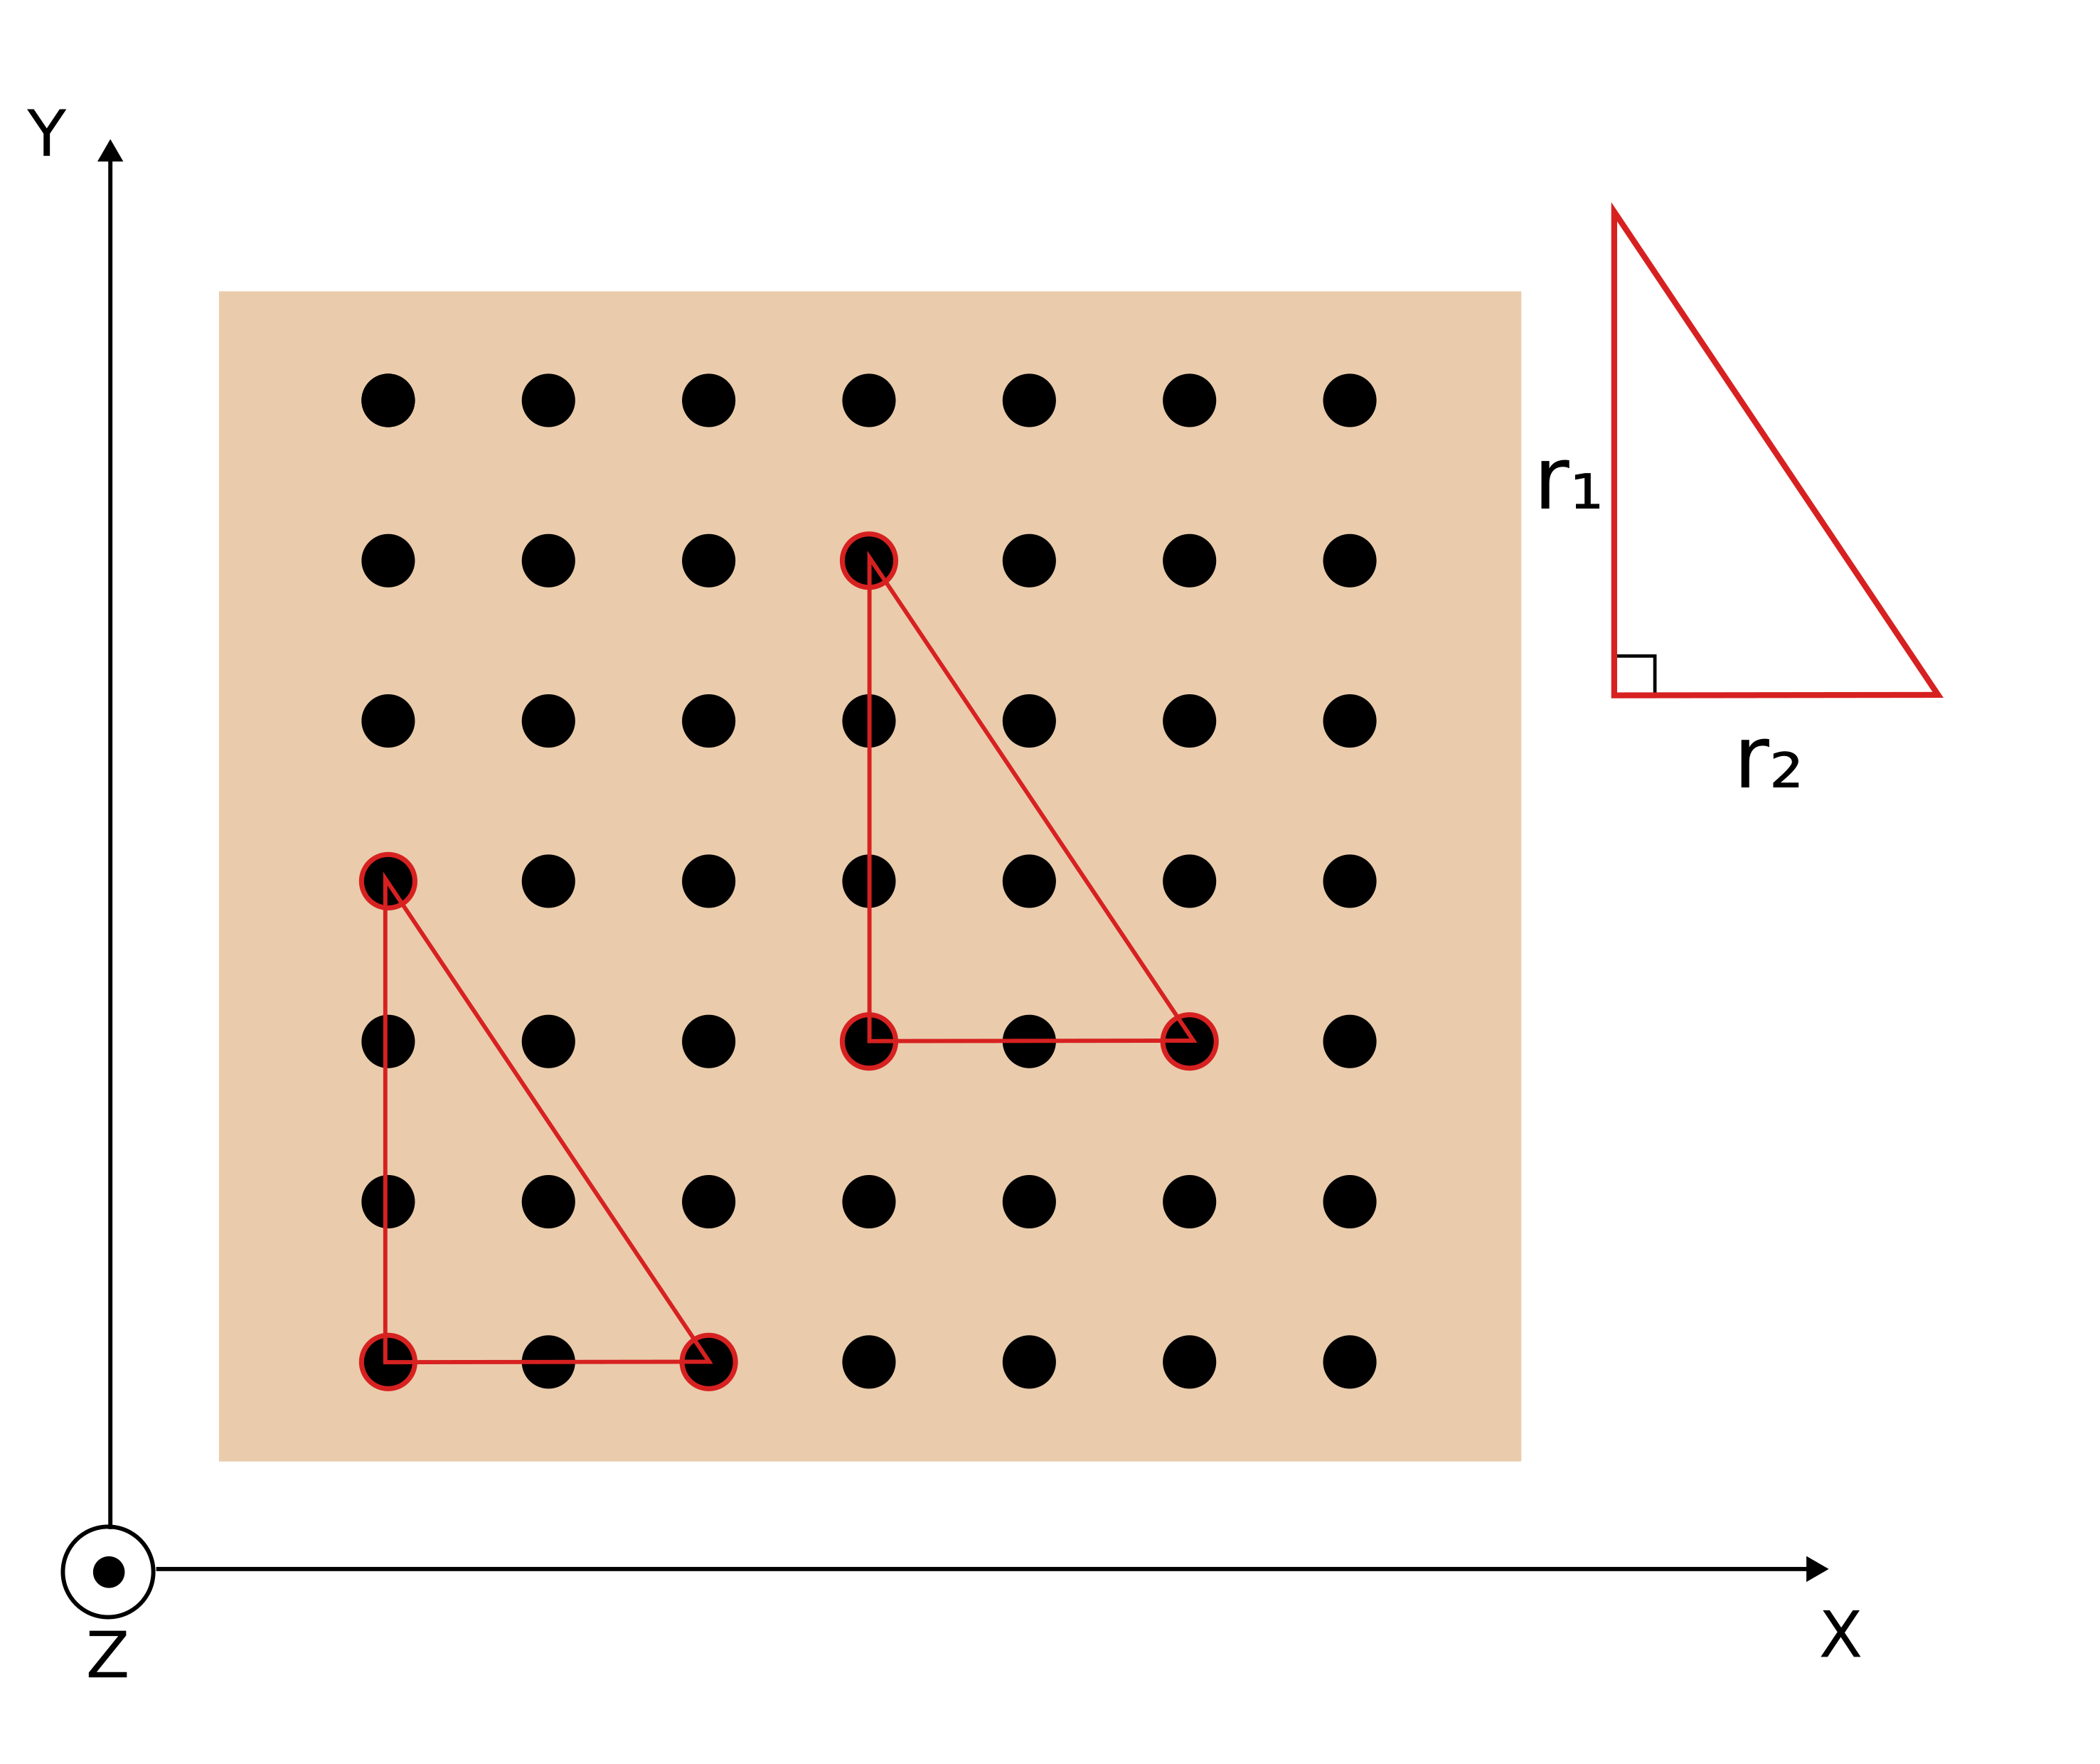
\includegraphics[width=0.6\linewidth]{images/pattern.png}
  \caption[]{Sampling pattern used for calculation of $F_{sss}$ in our
    implementation is a right triangle with fixed catets $r_1$ and $r_2$.
    Patterns can lie in planes $XY$ (as on the picture), $XZ$ or $YZ$. This
    pattern is moved over the input which results in all possible distinct
    configurations. Black dots depict elements of $A'$.}
  \label{fig:Fsss-pattern}
\end{figure}

\subsection{Betterment of the discrete approach with improved edge filter}
In this work, in addition to filter $H$, we propose an improved filter $H'$. The
rationale behind this improvement is that:
\begin{itemize}
\item a filter of width 3 may turn to be too narrow to give a good approximation
  for particular structures;
\item The filter $H$ is not invariant under rotations, i.e.
  $H*R(A) \ne R(H*A)$, where $R$ is a rotation operator.
\end{itemize}
Filter $H'$ has a length $7$ and all coefficients with exception to the central
coefficient are inversely proportional to the distance from the center:
\begin{equation}
  \begin{aligned}
    H'_{ij} &= S \left\{
    \begin{array}{cc}
      \frac{1}{\sqrt{(i-3)^2 + (j-3)^2}} & \quad i \ne 3, j \ne 3 \\
      C & \quad \text{otherwise}
    \end{array}
    \right. \\
    H'_{ijk} &= S \left\{
    \begin{array}{cc}
      \frac{1}{\sqrt{(i-3)^2 + (j-3)^2 + (k-3)^3}} & \quad i \ne 3, j \ne 3, k
      \ne 3 \\
      C & \quad \text{otherwise}
    \end{array}
    \right.
  \end{aligned}
  \label{eq:filter-7x7}
\end{equation}
where $C$ is such that all coefficients of $H'$ sum to zero, and $S$ equals to
$30.45849$ in 2D and $172.96232$ in 3D case.

\begin{figure}
  \centering
  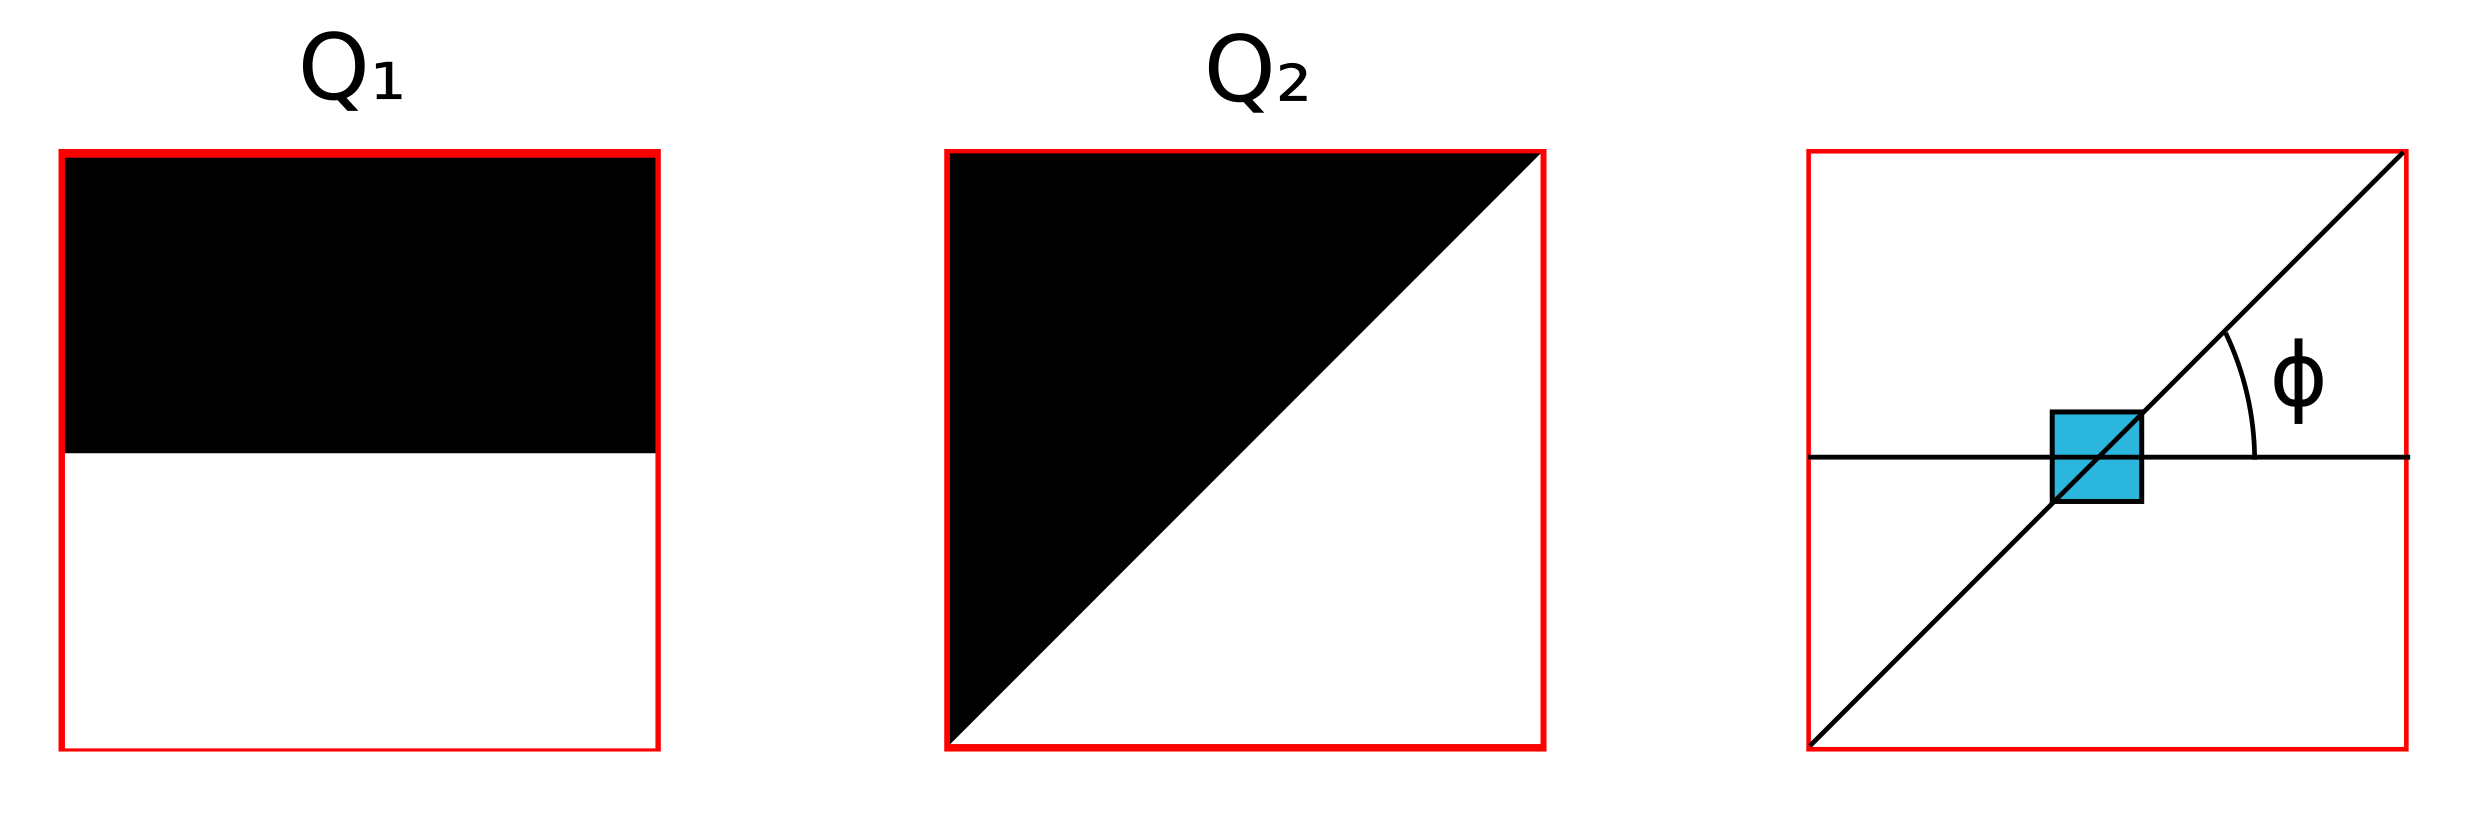
\includegraphics[width=\linewidth]{images/experiment-setup.png}
  \caption[]{Left, center: images $Q_1$ and $Q_2$ used in the demonstration of
    approximation for $1 / \sin \phi$. Right: Interfaces between phases are
    line segments which intersect each other at angle $\phi$. Shaded area is
    where $|(H*Q_1)\cdot(H*Q_2)|$ has non-zero values. Sum of all values in this
    area approximates $1 / \sin \phi$.}
  \label{fig:experiment-setup}
\end{figure}
Consider two 2D images like the ones on \cref{fig:experiment-setup}. Boundaries
between black and white areas cross each other at the angle $\phi$. We apply an
edge detection filter to each image, multiply results element-wise and sum all
elements of the product. We want the resulting value to approximate
$1/\sin \phi$. As can be seen on \cref{fig:filter-comparison} $H'$ does this job
better than $H$. Why this is important will be explained in \cref{sec:fss-2d}.
\begin{figure}
  \centering
  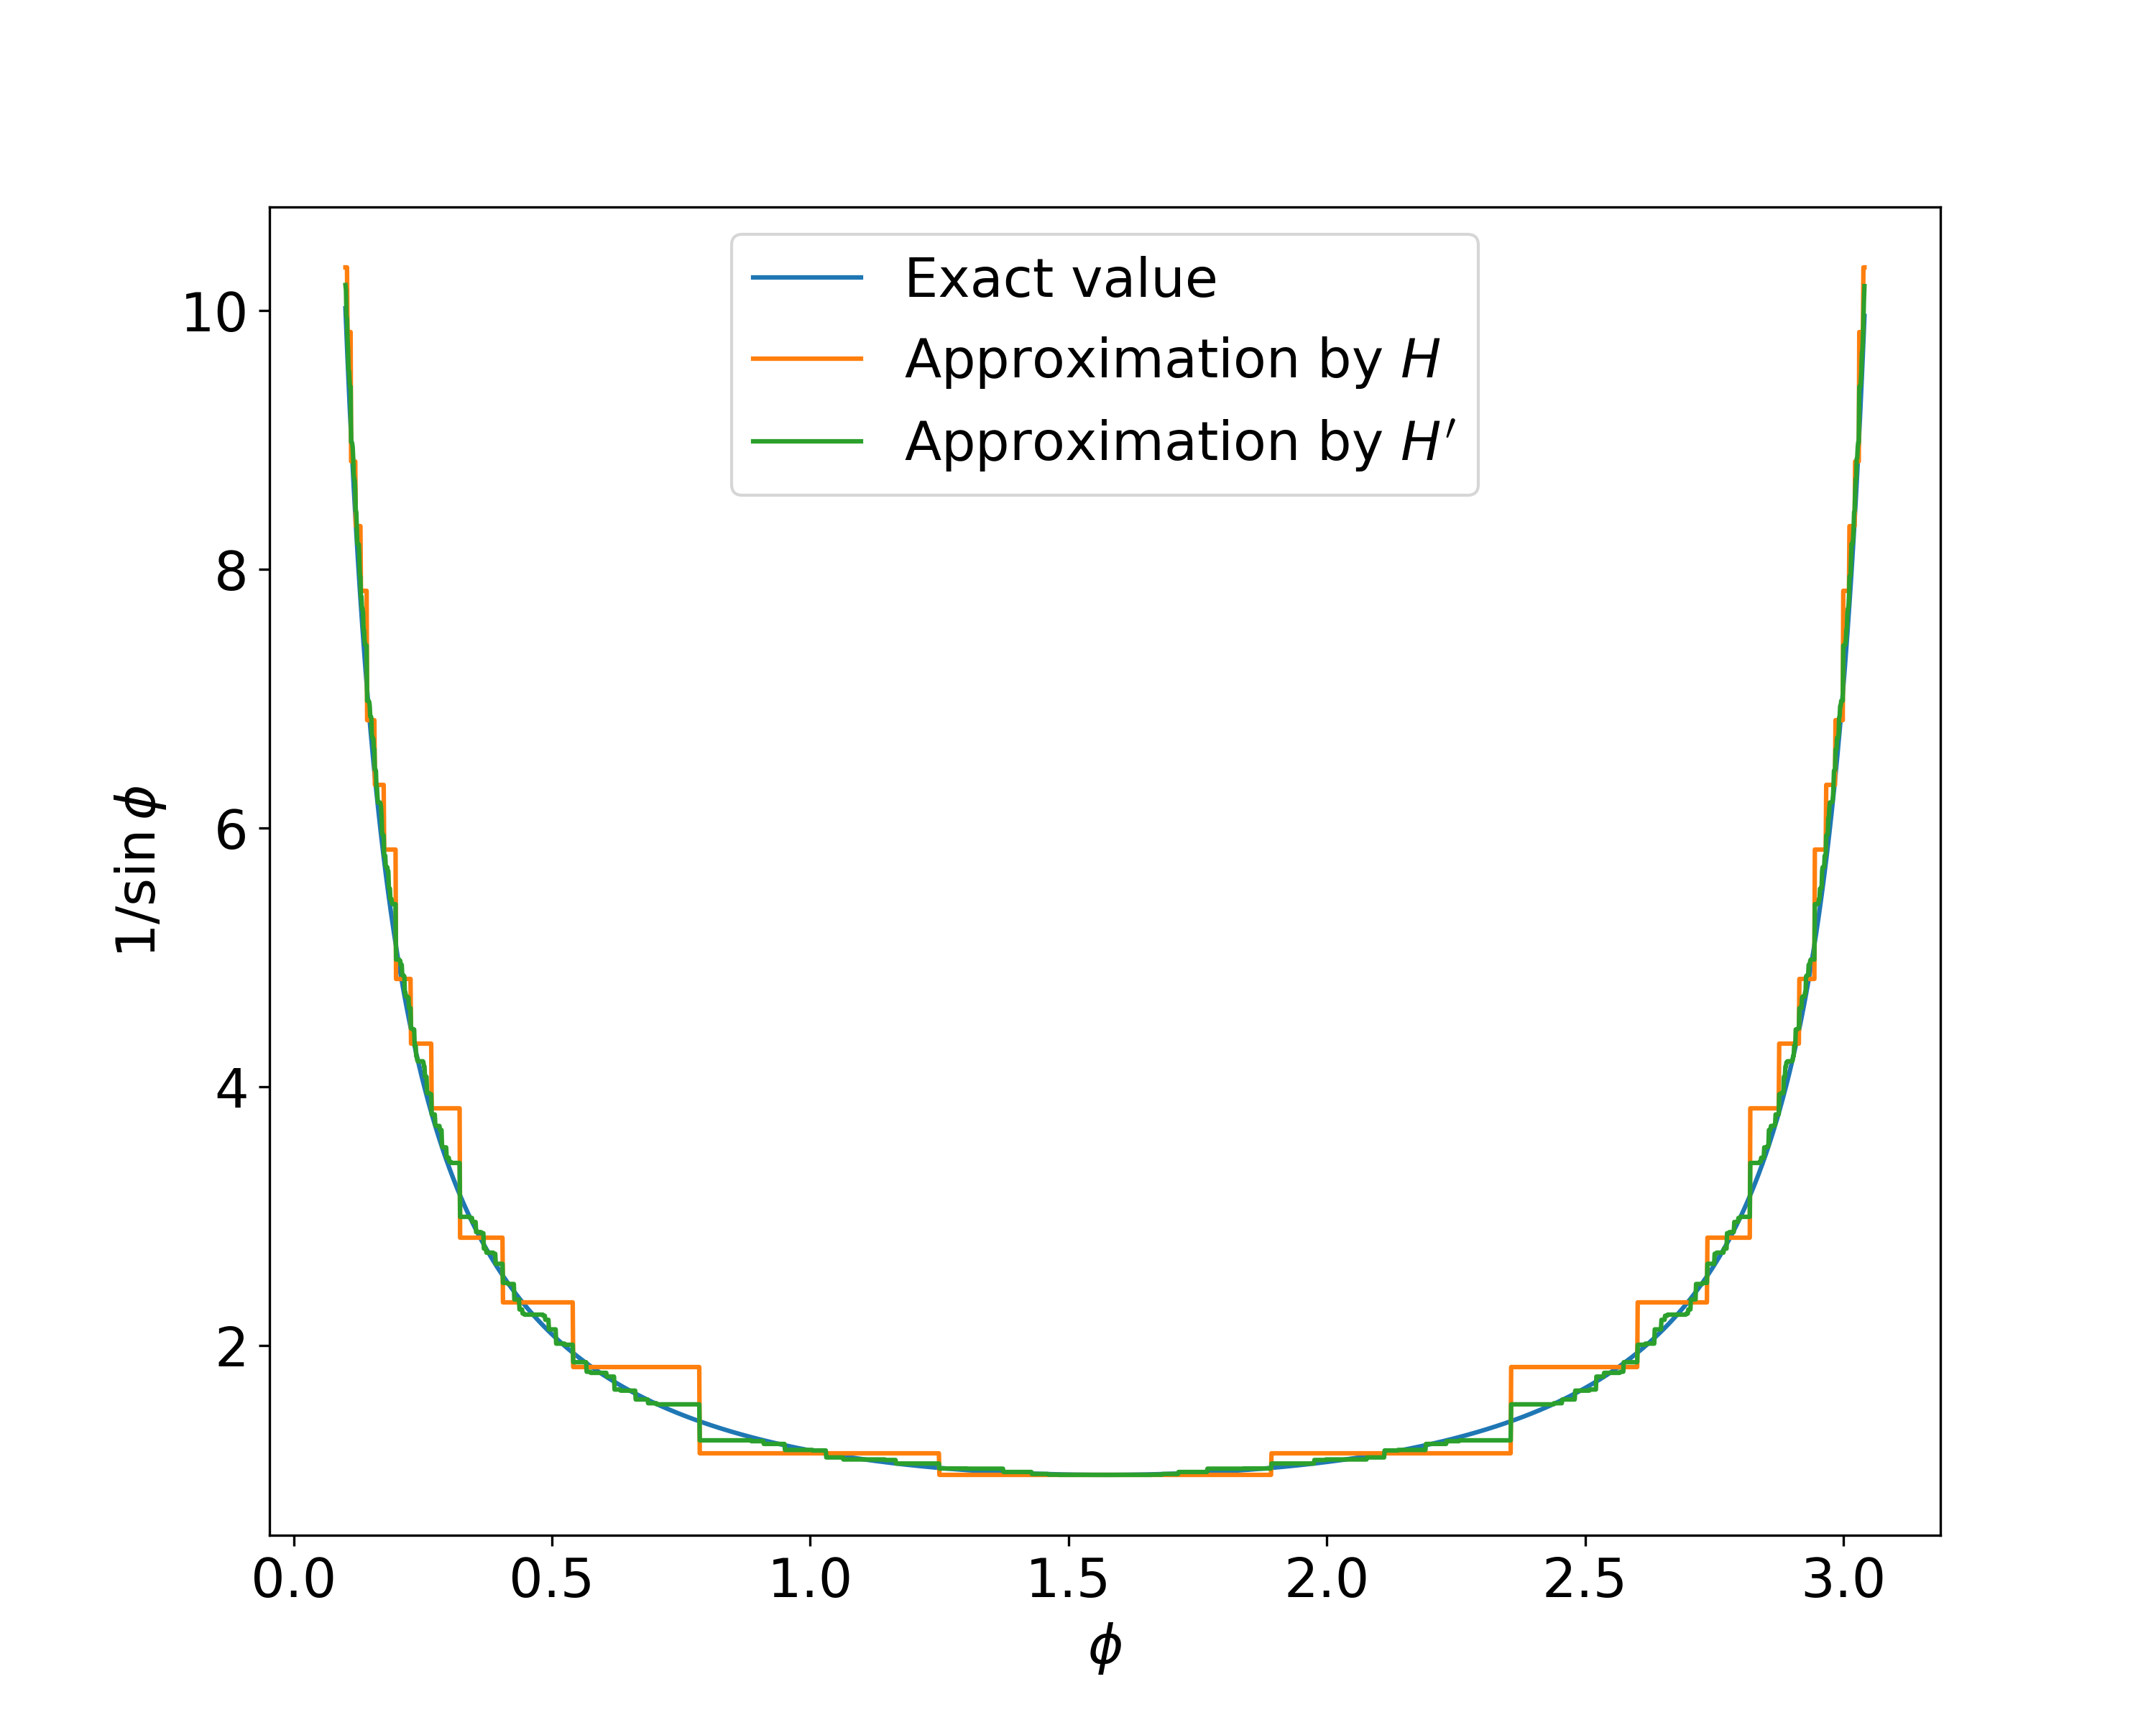
\includegraphics[width=0.6\linewidth]{images/filter-comparison.png}
  \caption[]{Estimation of $1/\sin\phi$ by filters $H$ and $H'$ for binary
    images on \cref{fig:experiment-setup}.}
  \label{fig:filter-comparison}
\end{figure}

\subsection{Units for computed surface correlation functions}
From now on we introduce a conventional unit of measurement ($cu$) for length.
When considering $F_{ss}$ and $F_{sv}$ functions we will work with square images
with side equal to $1\ cu$, so we can omit division by $N$ in described
algorithms and ensemble average in \cref{eq:fss} and \cref{eq:fsv} becomes a
double integral over a square $[0, 1]^2$. When considering $F_{sss}$ function we
will work with cubic images with side equal to $1\ cu$. Then we can also omit
division by $N$ and ensemble average in \cref{eq:fsss} becomes a triple integral
over a cube $[0, 1]^3$. On plots of surface functions we will omit units of
measurements in captions (e.g. we will write ``$F_{ss}$'' instead of
``$F_{ss}, cu^{-2}$'').

\section{Computation of surface functions for sets with smooth boundary}
\label{sec:algo-precise}
Previously \cite{Samarin} we tested algorithms for digital images against known
analytic solutions. Although we obtained good results in the cases of
overlapping balls and disks, weather our algorithm performs with the same high
accuracy in general is still an open question. In this section we develop a
universal test case and novel exact algorithm for calculation of $F_{ss}$ and
$F_{sss}$ functions for two- and three-dimensional sets with smooth boundary.

\subsection{$F_{ss}$ function for two-dimensional sets with smooth boundary}
\label{sec:fss-2d}
\begin{figure}
  \centering
  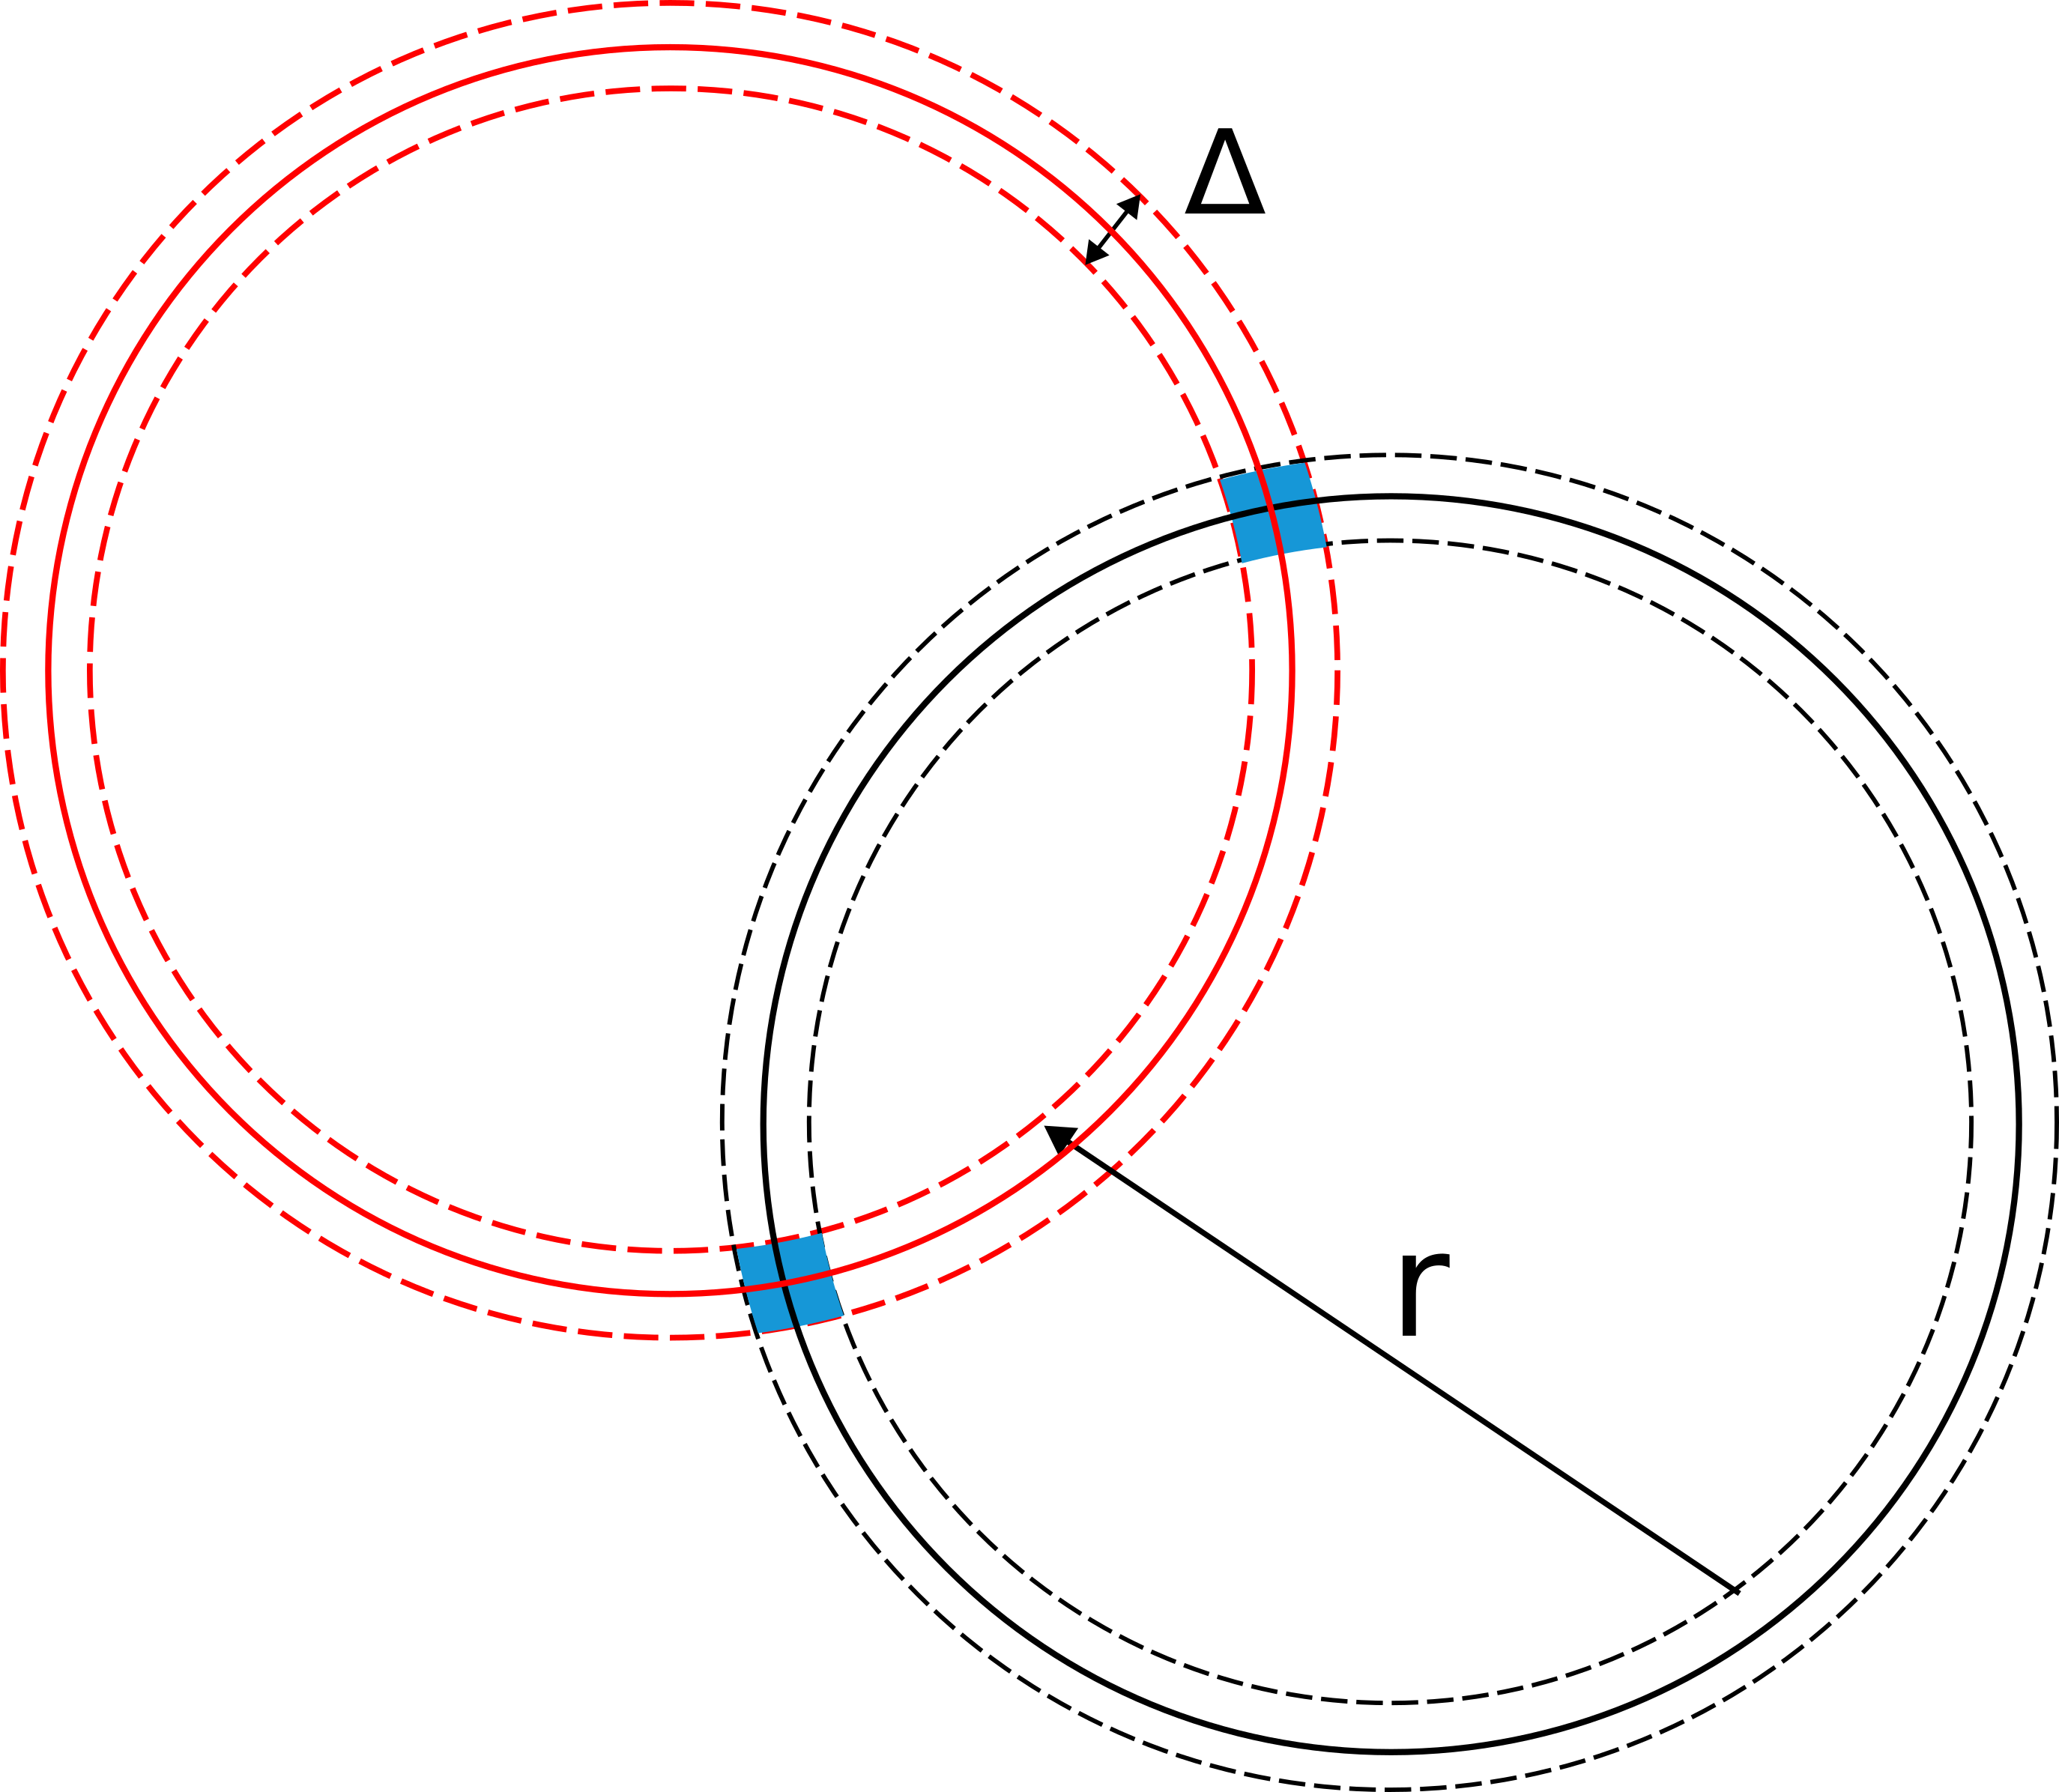
\includegraphics[width=0.6\linewidth]{images/Fss.png}
  \caption[]{Illustration of how $F_{ss}(\bm{r})$ is calculated. The interface
    between solid and void phases is a solid black curve. This interface
    translated by the vector $\bm{r}$ is show as a red solid curve. Support of
    $f_\Gamma(\bm{x}; \Delta)$ is a dashed ring. Shaded regions contribute to
    the surface-surface function.}
  \label{fig:Fss-explained}
\end{figure}
Let $S$ be some set in $\mathbb{R}^2$ which has a smooth boundary $\Gamma$ in
the sense that the boundary has a tangent line almost everywhere. Now we
introduce a function $f_\Gamma(\bm{x}; \Delta)$:
\begin{equation}
  f_\Gamma(\bm{x}; \Delta) = \left\{
  \begin{array}{ll}
    1/\Delta & \quad \rho(\bm{x}, \Gamma) < \Delta \\
    0 & \quad \text{otherwise}
  \end{array}
  \right. \label{eq:delta-sequence}
\end{equation}
Here $\rho(\bm{x}, \Gamma)$ means the closest distance from point $\bm{x}$ to the
boundary $\Gamma$.

\begin{figure}
  \centering
  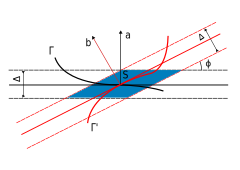
\includegraphics[width=0.6\linewidth]{images/fss-zoomed.png}
  \caption[]{Zoomed image of intersection between the interface $\Gamma$ and its
    translated version $\Gamma'$. $\phi$ is an angle between tangent lines to
    the interfaces. Surface of dashed area is
    $\frac{\Delta^2}{\sin \phi}$. Vectors $\bm{a}$ and $\bm{b}$ are unit vectors
    parallel to normals to $\Gamma$ and $\Gamma'$ respectively in the point of
    their intersection.}
  \label{fig:fss-zoomed}
\end{figure}
Now define a functional sequence $F_{ss}(\bm{r}; \Delta)$:
\begin{equation}
  \begin{aligned}
    F_{ss}(\bm{r}; \Delta) &= \int\int f_\Gamma(\bm{x}; \Delta) f_\Gamma(\bm{x}
    + \bm{r}; \Delta) dx dy \\
    &= \sum_{k=1}^N S_k/\Delta^2
  \end{aligned}
\end{equation}
Here $N$ is a number of intersections of $\Gamma$ with itself translated by a
vector $\bm{r}$ and $S_k$ is a surface of each such intersection (see
\cref{fig:Fss-explained}).
When $\Delta$ tends to zero, the boundary at the point of intersection can
be replaced with a tangent line at the point of intersection
(\cref{fig:fss-zoomed}). Thus, we get an expression for a surface of
intersection: $S_k = \frac{\Delta^2}{\sin \phi_k}$ where $\phi_k$ is an
acute angle between tangent lines. Hence, we obtain the following equation:
\begin{equation}
  F_{ss}(\bm{r}) = \lim_{\Delta \to 0} F_{ss}(\bm{r}; \Delta) =
  \sum_{k=1}^N \frac{1}{\sin \phi_k} \label{eq:fss-2d-sin}
\end{equation}
It's easy to show that
$\lim_{\Delta \to 0} f_\Gamma(\bm{x}; \Delta) = |\nabla \chi_A(\bm{x})|$
and, therefore, \cref{eq:fss-2d-sin} and \cref{eq:fss} define the same
function. This equation for $F_{ss}$ also explains why edge detection filters
need to approximate $1/\sin \phi_k$ and why the filter \cref{eq:filter-7x7} is
better than \cref{eq:filter-3x3}.

A less illustrative but more practical way to calculate an expression
$\frac{S_k}{\Delta}$ is the following. Take two vectors $\bm{a}$ and $\bm{b}$
parallel to normals to $\Gamma$ and $\Gamma'$ in $k$-th point of their
intersection such as $|a| = |b| = 1$. If $F_{ss}$ is defined at the point of
consideration then $\bm{a} \ne \pm \bm{b}$. The pair $(\bm{a}, \bm{b})$ may
serve as a basis with the following transformation from the basis
$(1,0), (0,1)$:
\begin{equation}
  \begin{aligned}
    x' &= f(x, y) = a_x x + a_y y \\
    y' &= g(x, y) = b_x x + b_y y
  \end{aligned}
\end{equation}
where $\bm{a} = (a_x, a_y)$, $\bm{b} = (b_x, b_y)$. Jacobian determinant for
this transformation is:
\begin{equation}
  J = \left|
  \begin{array}{cc}
    \frac{\partial f}{\partial x} & \frac{\partial f}{\partial y} \\
    \frac{\partial g}{\partial x} & \frac{\partial g}{\partial y} \\
  \end{array}
  \right| =
  \left|
  \begin{array}{cc}
    a_x & a_y \\
    b_x & b_y
  \end{array}
  \right| = a_x b_y - a_y b_x
\end{equation}

We can rewrite \cref{eq:fss-2d-sin} using $J$ as follows:
\begin{equation}
  F_{ss}(\bm{r}) = \sum_{k=1}^N \frac{1}{|J_k|} \label{eq:fss-2d}
\end{equation}
where $J_k$ is Jacobian determinant computed at $k$-th point of
intersection. This form proves to be much more useful than the version which
contains the angle $\phi$.

Now we get to practical algorithm for computation of $F_{ss}$ for sets with a
smooth boundary. Suppose a set $S$ is defined as
$S = \left\{ (x, y) \ | \quad f(x, y) \le T \right\}$ where $f(x, y)$ is some
function differentiable at points where $f(x, y) = T$ and $T$ is some
threshold. Let's calculate surface-surface function for this set at a point
$\bm{r} = (r_x, r_y)$. We find all intersections between a boundary $\Gamma$ and
its translated version by solving a system of equations:
\begin{equation}
  \left\{
  \begin{array}{l}
    f(x, y) = T \\
    f(x-r_x, y-r_y) = T
  \end{array}
  \right.
\end{equation}
which can now be replaced by a single equation:
\begin{equation}
  (f(x, y) - T)^2 + (f(x-r_x, y-r_y) - T)^2 = 0 \label{eq:inter}
\end{equation}
We denote a set of solutions of this equation as $X$. For every $\bm{x}_i \in X$
we find normals to the boundary and the boundary translated by a vector
$\bm{r}$. These normals can be found using automatic differentiation and dual
numbers described in \ref{sec:dual}. Then we normalize these vectors and use
\cref{eq:fss-2d} to calculate $F_{ss}$.

Summarizing, the algorithm of calculating $F_{ss}(\bm{r})$ is the following:
\begin{enumerate}
\item Find $X$ which is a set of solutions of \cref{eq:inter}.
\item For all points in $X$ find normals to the boundaries using
  \cref{eq:autonormals} and normalize them.
\item Calculate $F_{ss}(\bm{r})$ using \cref{eq:fss-2d}.
\end{enumerate}

The set $X$ can be found by firstly evaluating $f(x, y)$ in some regular grid
searching for all points $(x_i, y_i)$ for which $|f(x_i, y_i) - T| < \epsilon$
and $|f(x_i - r_x, y_i - r_y) - T| < \epsilon$ for some positive $\epsilon$ 
(small value does not affect computation results, $\epsilon=0.04$ was used in
all cases in this work) and then using these points as starting points for some
algorithm based on gradient descent (ADAM \cite{adam} was used in this work) to
solve \cref{eq:inter}.

\subsection{$F_{sss}$ function for three-dimensional sets with smooth boundary}
\label{sec:fsss-3d}
Results of this section are made by analogy with \cref{sec:fss-2d}. Again, let
$S$ be some set in $\mathbb{R}^3$ which has a smooth boundary, i.e. has a
tangent plane at almost every point of its boundary. Using the function
\cref{eq:delta-sequence} we define a functional sequence
$F_{sss}(\bm{r_1}, \bm{r_2}; \Delta)$:
\begin{equation}
  \begin{aligned}
    F_{sss}(\bm{r_1}, \bm{r_2}; \Delta) &= \int\int\int dx dy dz \times \\
    &\qquad \times f_\Gamma(\bm{x}; \Delta) f_\Gamma(\bm{x} + \bm{r_1}; \Delta)
    f_\Gamma(\bm{x} + \bm{r_2}; \Delta) \\
    &= \sum_{k=1}^N V_k/\Delta^3
  \end{aligned}
\end{equation}
where $V_k$ is a volume of parallelepiped where all three multiplicands under
integral are non-zero. $N$ is a number of these parallelepipeds, i.e. number of
points where all three boundaries (one ``original'' boundary and two translated
versions) have an intersection. With $\Delta$ going to zero we get a convergence
to $F_{sss}$:
\begin{equation}
  \lim_{\Delta \to 0} F_{sss}(\bm{r_1}, \bm{r_2}; \Delta) = F_{sss}(\bm{r_1},
  \bm{r_2})
\end{equation}

Let $\bm{a}$, $\bm{b}$ and $\bm{c}$ be normalized normals to each boundary in
the point of intersection. The corresponding $V_k$ is finite if and only if
$\bm{a} \ne \pm \bm{b} \ne \pm \bm{c}$. In this case we can use a triplet
$(\bm{a}, \bm{b}, \bm{c})$ as basis for $\mathbb{R}^3$ with the following
transformation from the basis $(1,0,0), (0,1,0), (0, 0, 1)$:
\begin{equation}
  \begin{aligned}
    x' &= f(x, y) = a_x x + a_y y + a_z z \\
    y' &= g(x, y) = b_x x + b_y y + b_z z \\
    z' &= h(x, y) = c_x x + c_y y + c_z z
  \end{aligned}
\end{equation}
The Jacobian determinant for this transformation is:
\begin{equation}
  J = \left|
  \begin{array}{ccc}
    a_x & a_y & a_z \\
    b_x & b_y & b_z \\
    c_x & c_y & c_z
  \end{array}
  \right|
\end{equation}
and the expression for $F_{sss}$ becomes:
\begin{equation}
  F_{sss}(\bm{r_1}, \bm{r_2}) = \sum_{k=1}^N \frac{1}{|J_k|} \label{eq:fsss-3d}
\end{equation}
where $J_k$ is Jacobian determinant computed at $k$-th point of
intersection.

\section{Verification and computation results}
\label{sec:results}
In this section we consider a variety of examples of sets for which the developed
precise algorithm is applicable. We intercompare surface-surface functions
calculated with the algorithm for digital images (\cref{sec:algo}) with results
of the novel continuous algorithm. We also demonstrate the work of both filter
$H$ (\ref{eq:filter-3x3}) for edge detection along with a new filter $H'$
(\ref{eq:filter-7x7}) proposed in this paper. Both digital and
continuous methods are verified against available analytical solutions.

\subsection{A square and a cube}
Define a function $f(\bm{x}) = \max\limits_i |x_i|$. A set $f(\bm{x}) \le T$
where $\bm{x} \in \mathbb{R}^2$ is a square with side $2T$. The function $f$ is
differentiable at all points where $f(\bm{x}) = T$ with exception to points
$(-T, -T)$, $(-T, T)$, $(T, -T)$ and $(T, T)$. The surface-surface correlation
function for a square is equal to:
\begin{equation}
  F_{ss}(\bm{r}) = \left\{
  \begin{array}{ll}
    2 & \quad f(\bm{r}) < 2T \ \text{and}\ r_i \ne 0, \forall i \in \overline{1,2} \\
    0 & \quad f(\bm{r}) > 2T \\
    \text{undefined} & \quad \text{otherwise}
  \end{array}
  \right.
\end{equation}
A graphical diagram depicting this case is shown on \cref{fig:fss-square}. In
this case the algorithm described in \cref{sec:algo} gives a correct result in
any point which is few pixels away from where $F_{ss}$ is undefined.
\begin{figure}
  \centering
  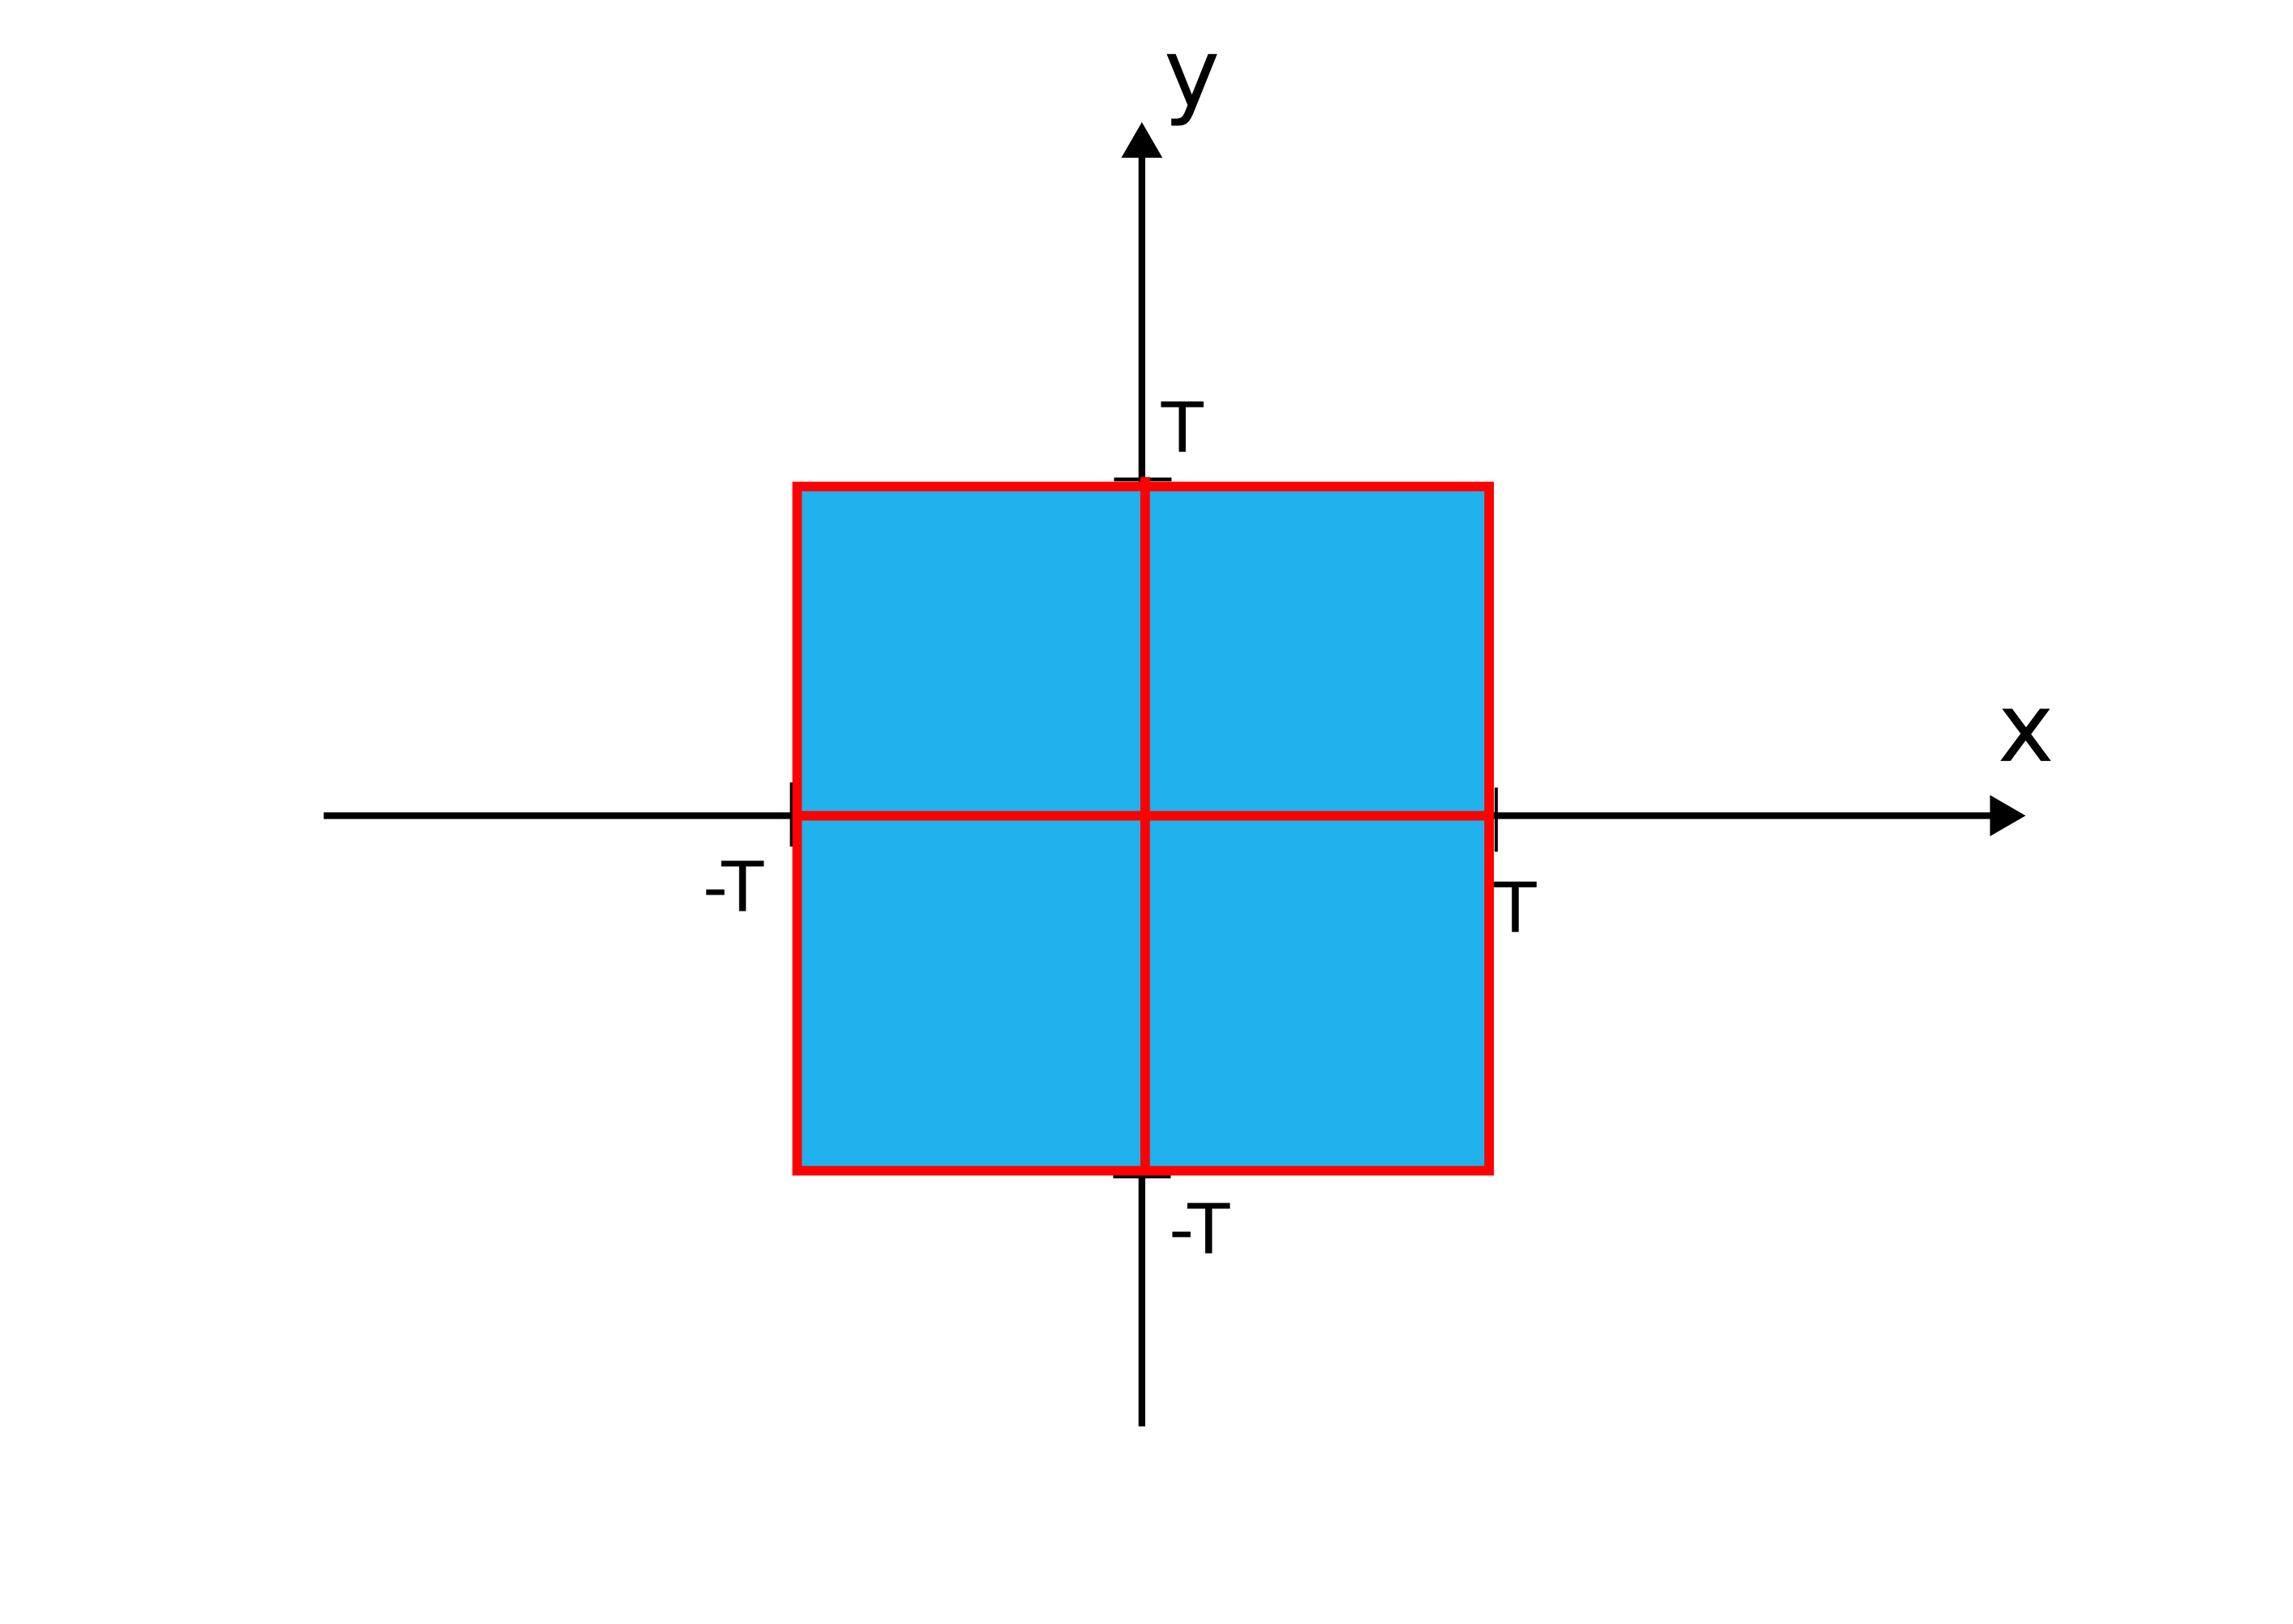
\includegraphics[width=0.45\linewidth]{images/fss-square.png}
  \hfill
  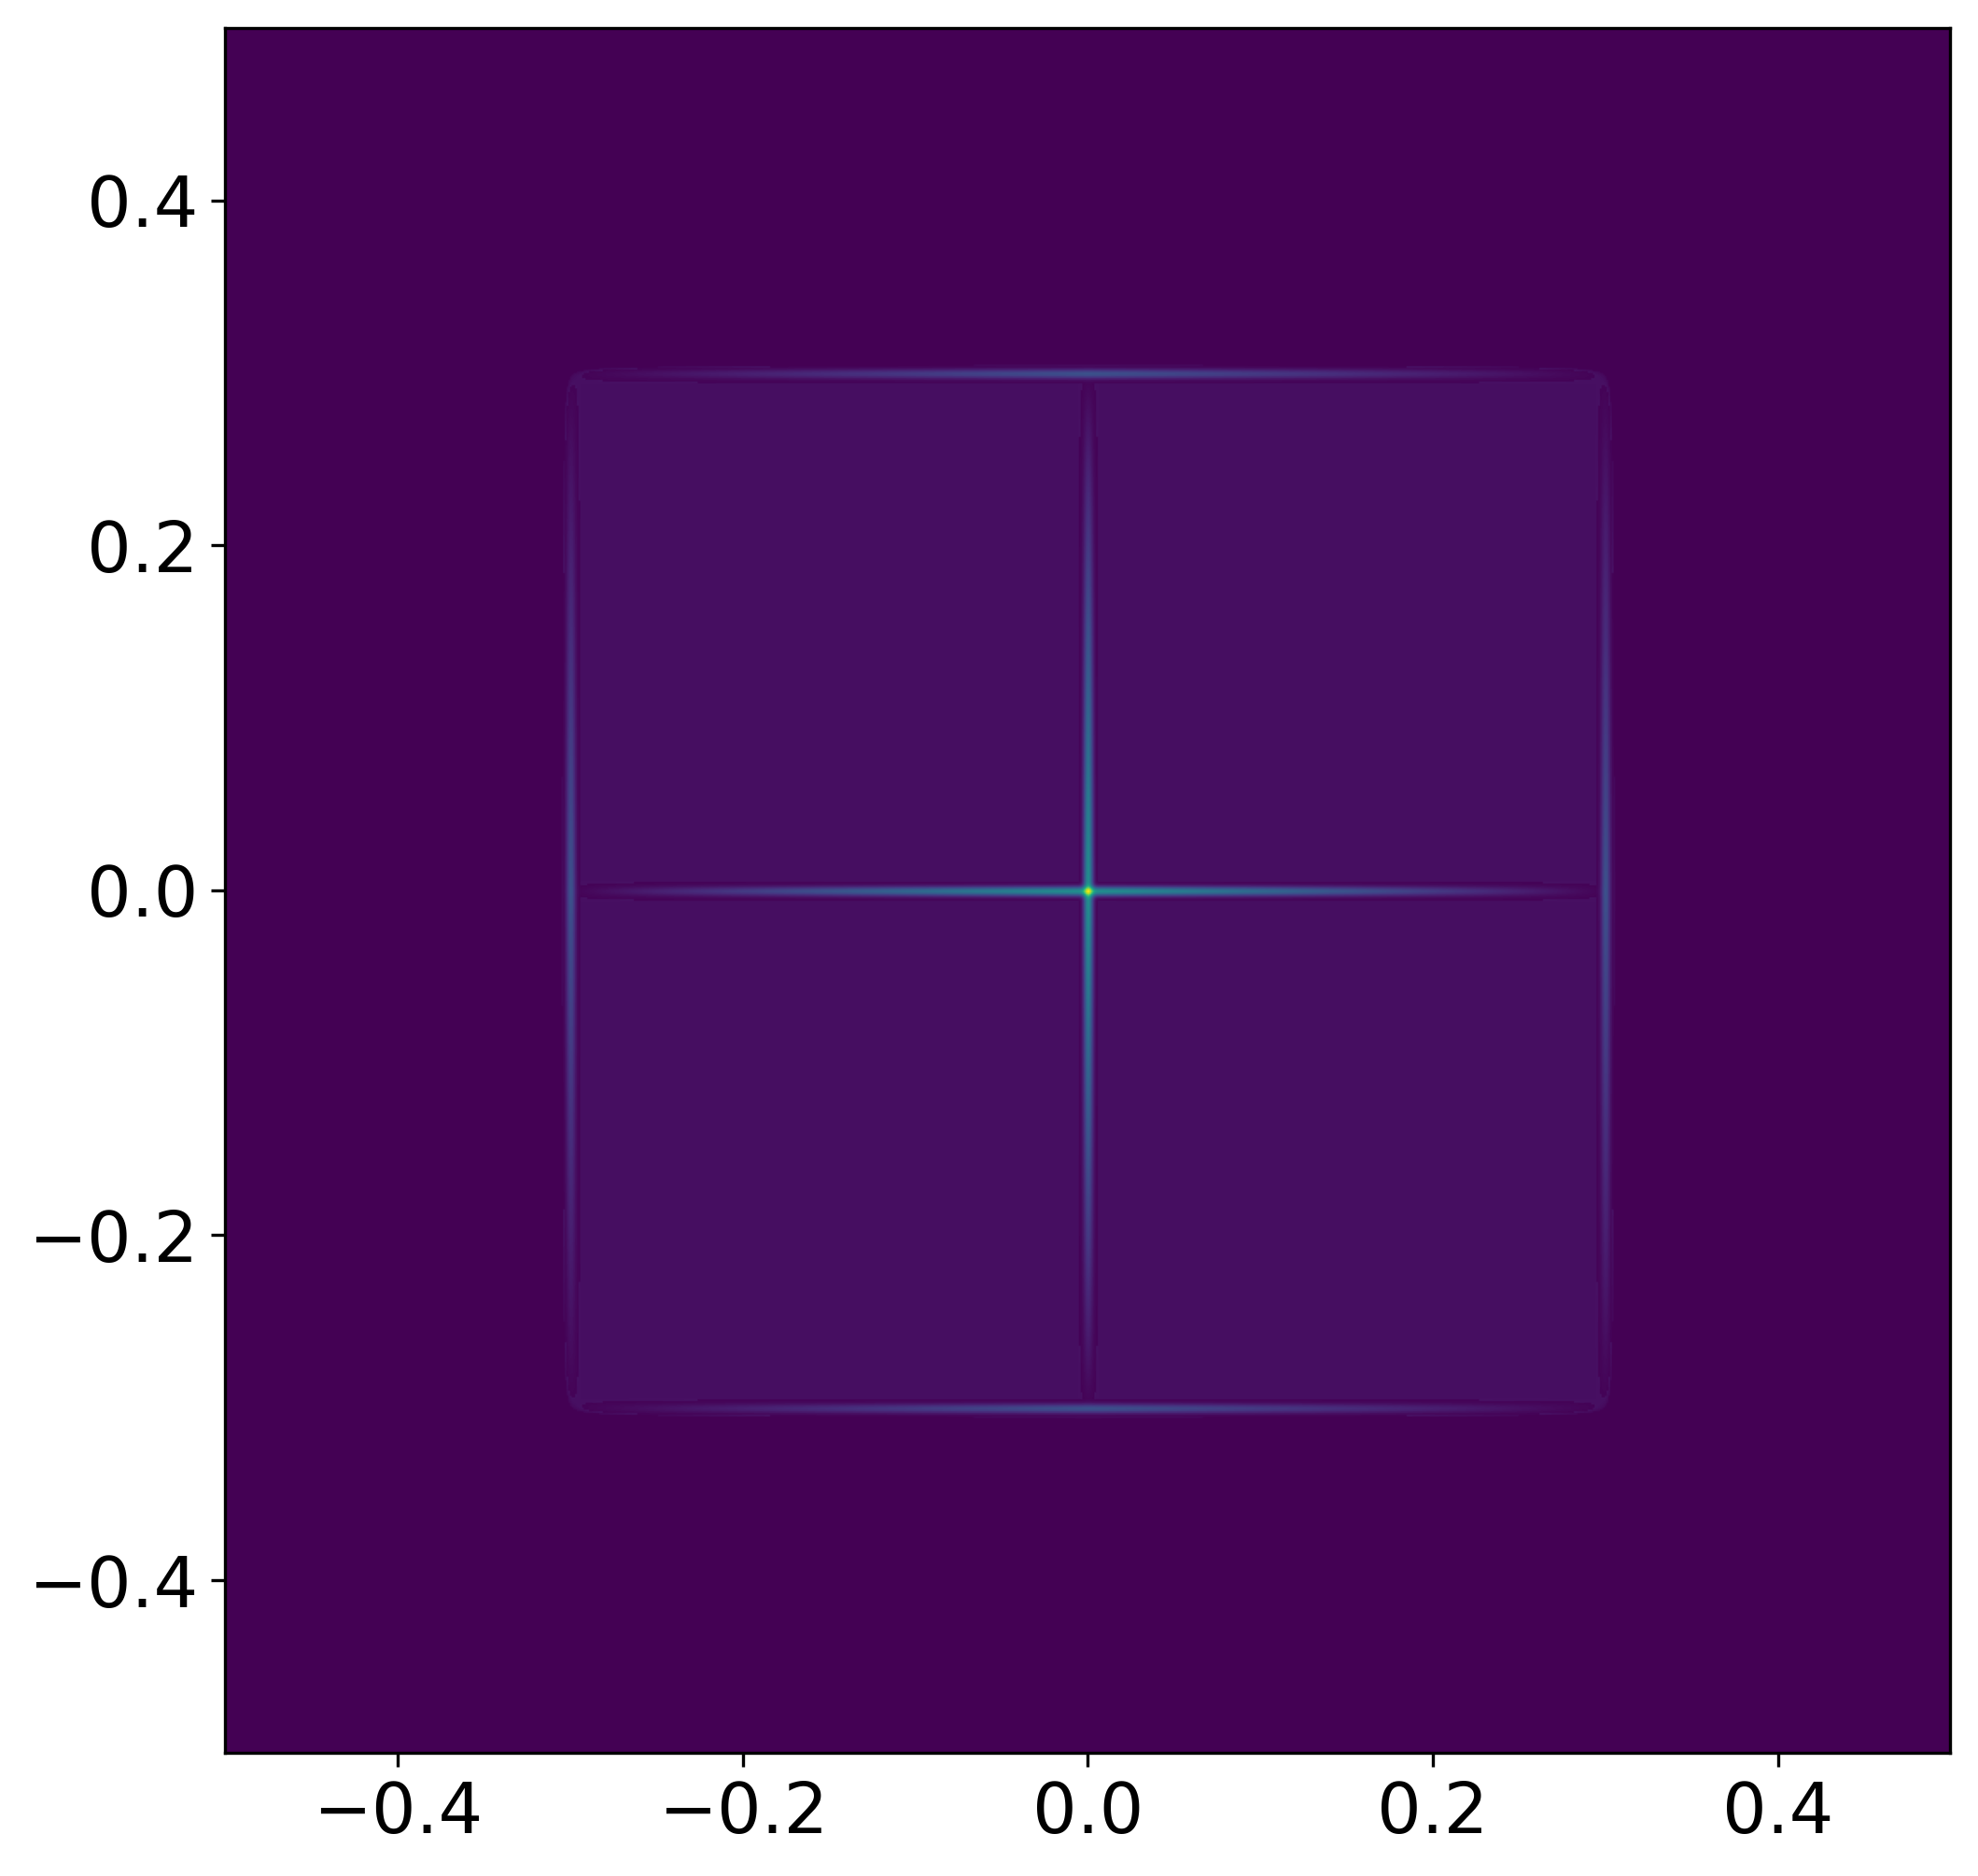
\includegraphics[width=0.45\linewidth]{images/fss-square-julia.png}
  \caption[]{$F_{ss}$ function for a square with side $T = 0.3$. On the left:
    Theoretical results. The function is undefined along red segments. Its value
    is $2$ inside a shaded area and $0$ outside. On the right: Calculation with
    the algorithm described in \cref{sec:algo}.}
  \label{fig:fss-square}
\end{figure}

A set $f(\bm{x}) \le T$ where $\bm{x} \in \mathbb{R}^3$ is a cube with the same
side $2T$.
The surface-surface-surface correlation function for this cube is equal to:
\begin{equation}
  F_{sss}(\bm{r}) = \left\{
  \begin{array}{ll}
    2 & \quad f(\bm{r}) < 2T \ \text{and}\ r_i \ne 0, \forall i \in \overline{1,3} \\
    0 & \quad f(\bm{r}) > 2T \\
    \text{undefined} & \quad \text{otherwise}
  \end{array}
  \right.
\end{equation}
This case is also handled perfectly by the algorithm described in
\cref{sec:algo}. Plot of $F_{sss}$ for the cube is trivially similar to
\cref{fig:fss-square} and, thus, not shown here. We conclude that all approaches
perform equally accurately for this simple test.

\subsection{A disk and a ball}
Define $f(\bm{x}) = \sum_i x_i^2$. If $\bm{x} \in \mathbb{R}^2$ when an
inequation $f(\bm{x}) \le R^2$ defines a disk of radius $R$ with the center at
the origin. In this case $F_{ss}$ depends only on distance $r$ from the origin:
\begin{equation}
  F_{ss}(r) = \left\{
  \begin{array}{ll}
    \frac{4R^2}{r\sqrt{4R^2-r^2}} & \quad r < 2R \\
    0 & \quad \text{otherwise}
  \end{array}
  \right.
\end{equation}
The comparison of the algorithm described in \cref{sec:algo} applied to images
with different resolution against theory is shown on \cref{fig:fss-disk}.
Continuous approach results for the disk coincide with analytical $F_{ss}$ function.
\begin{figure*}[!hpt]
  \centering
  \subfigure[$3\times 3$ kernel $H$]{
    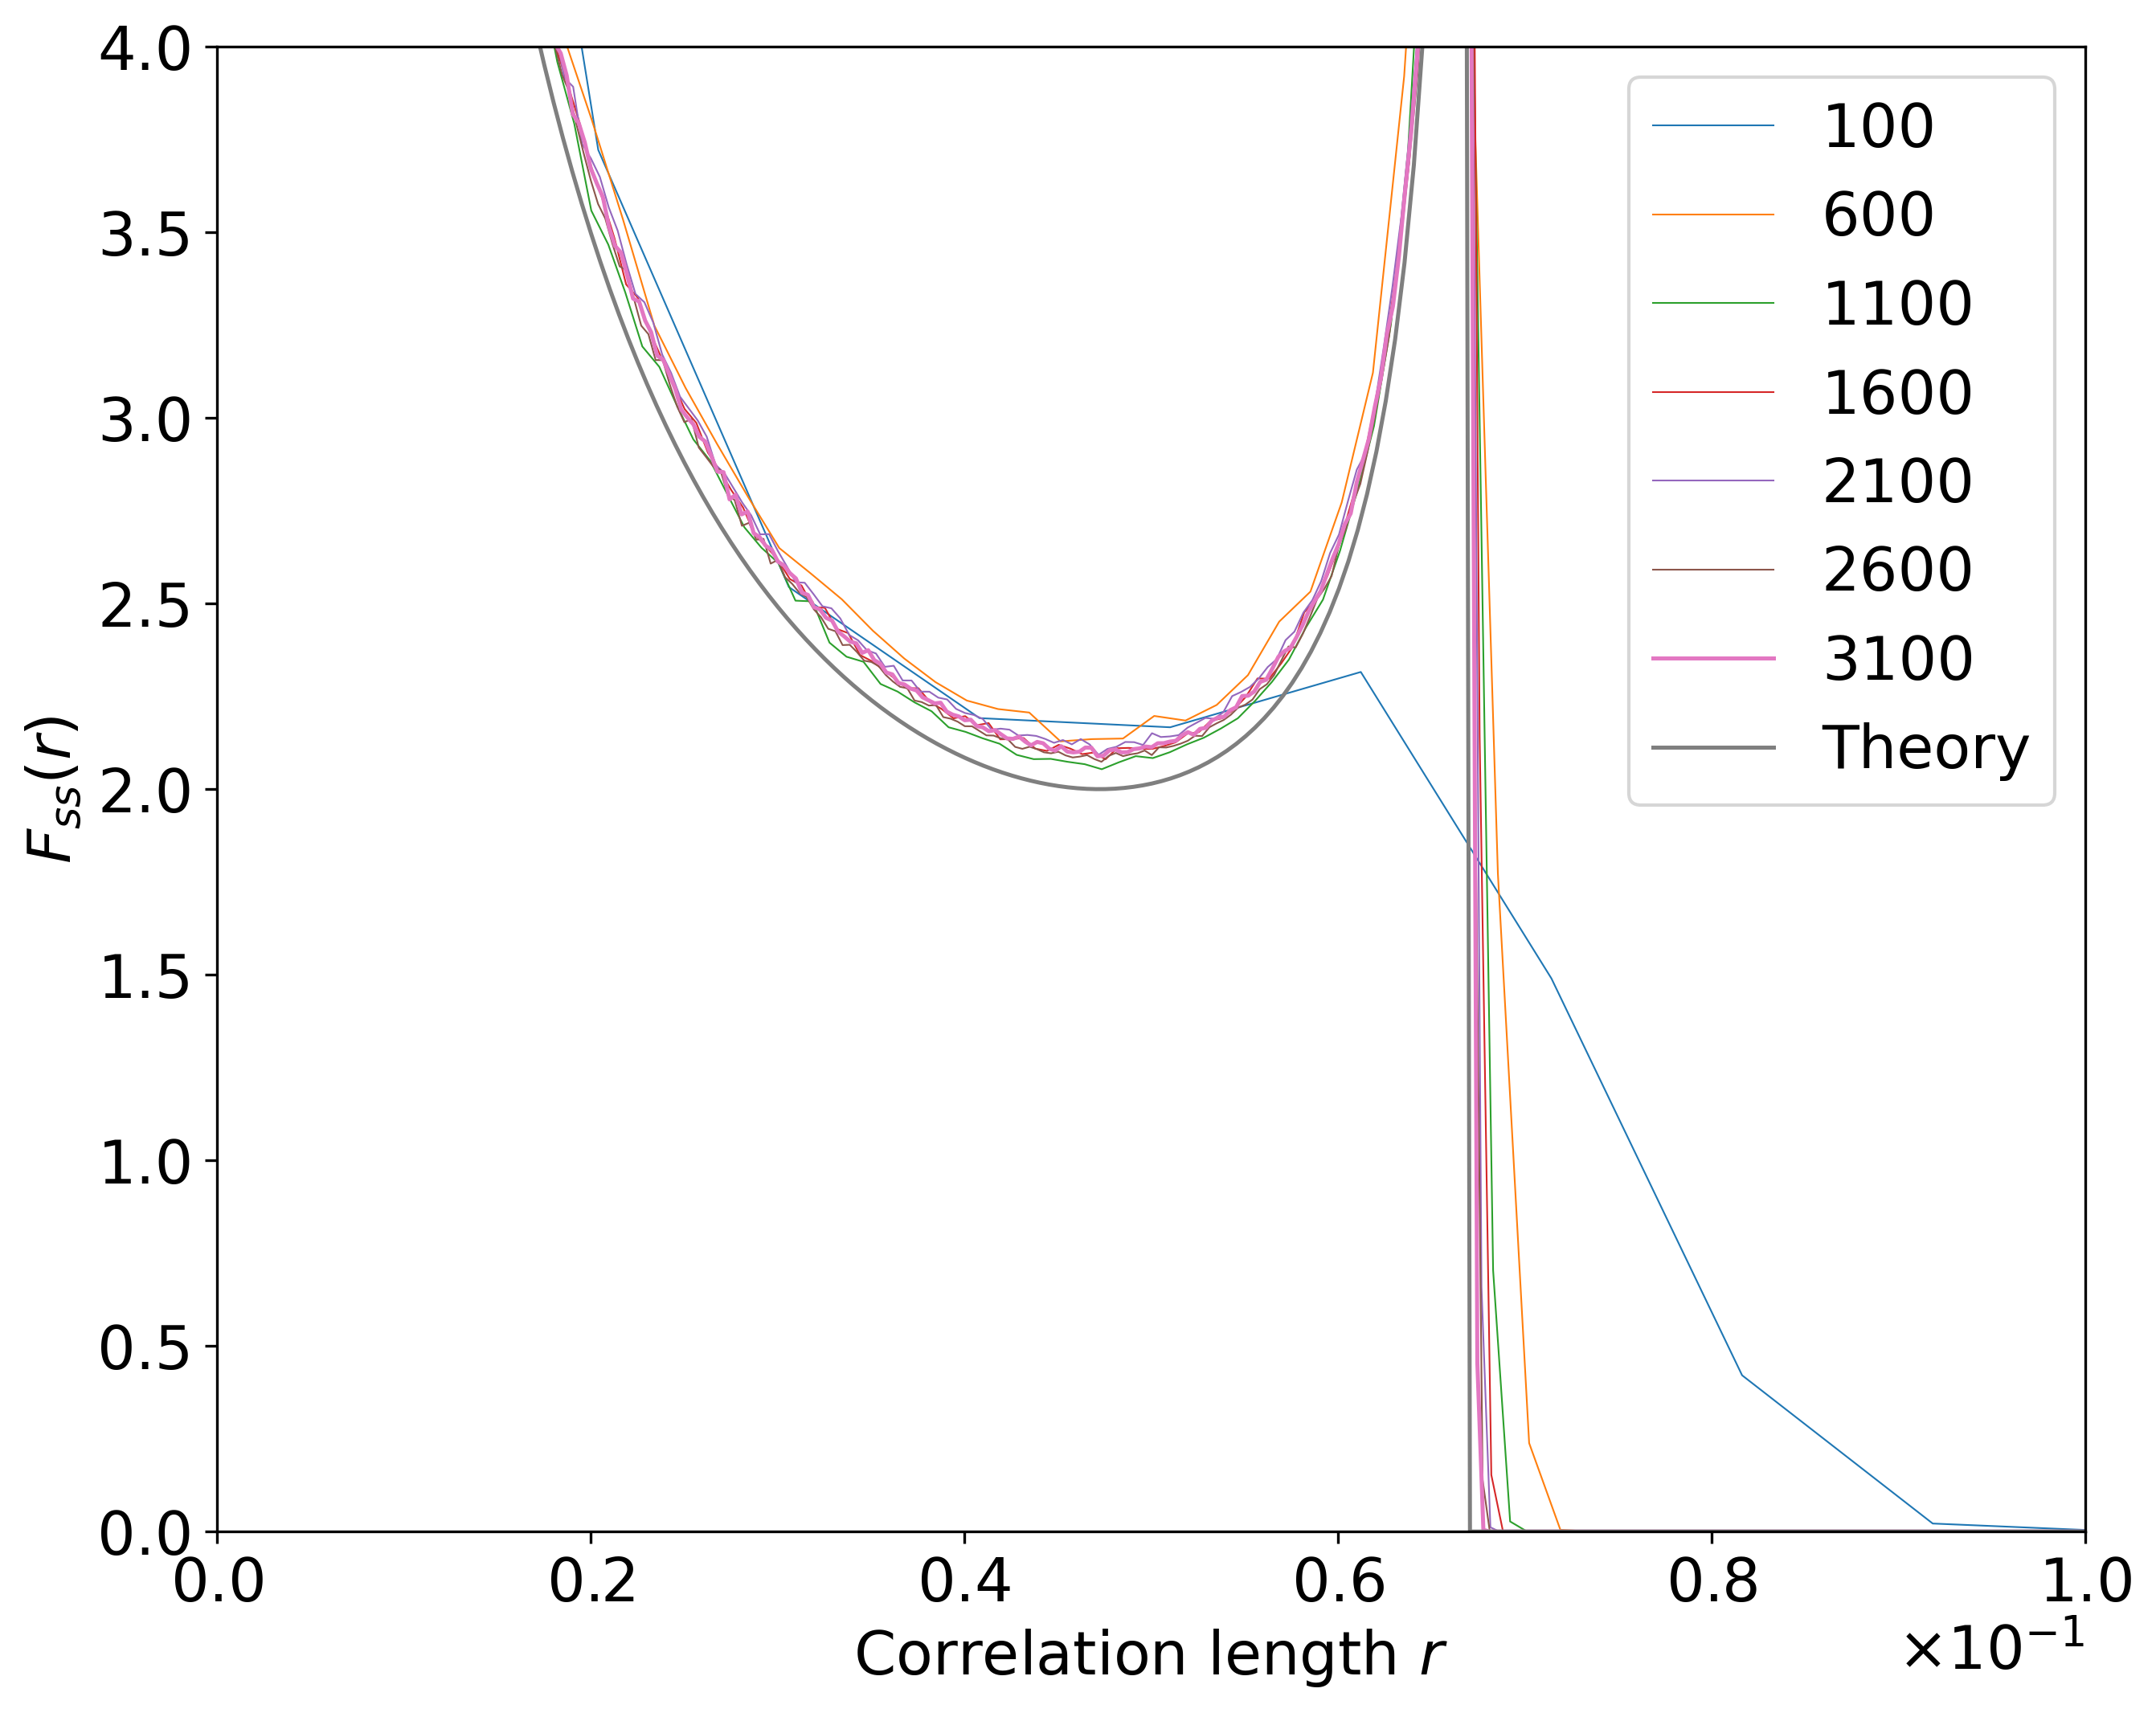
\includegraphics[width=0.45\linewidth]{images/fss-disk-3x3.png}
    \label{fig:fss-disk-3x3}}
  \hfill
  \subfigure[$7\times 7$ kernel $H'$]{
    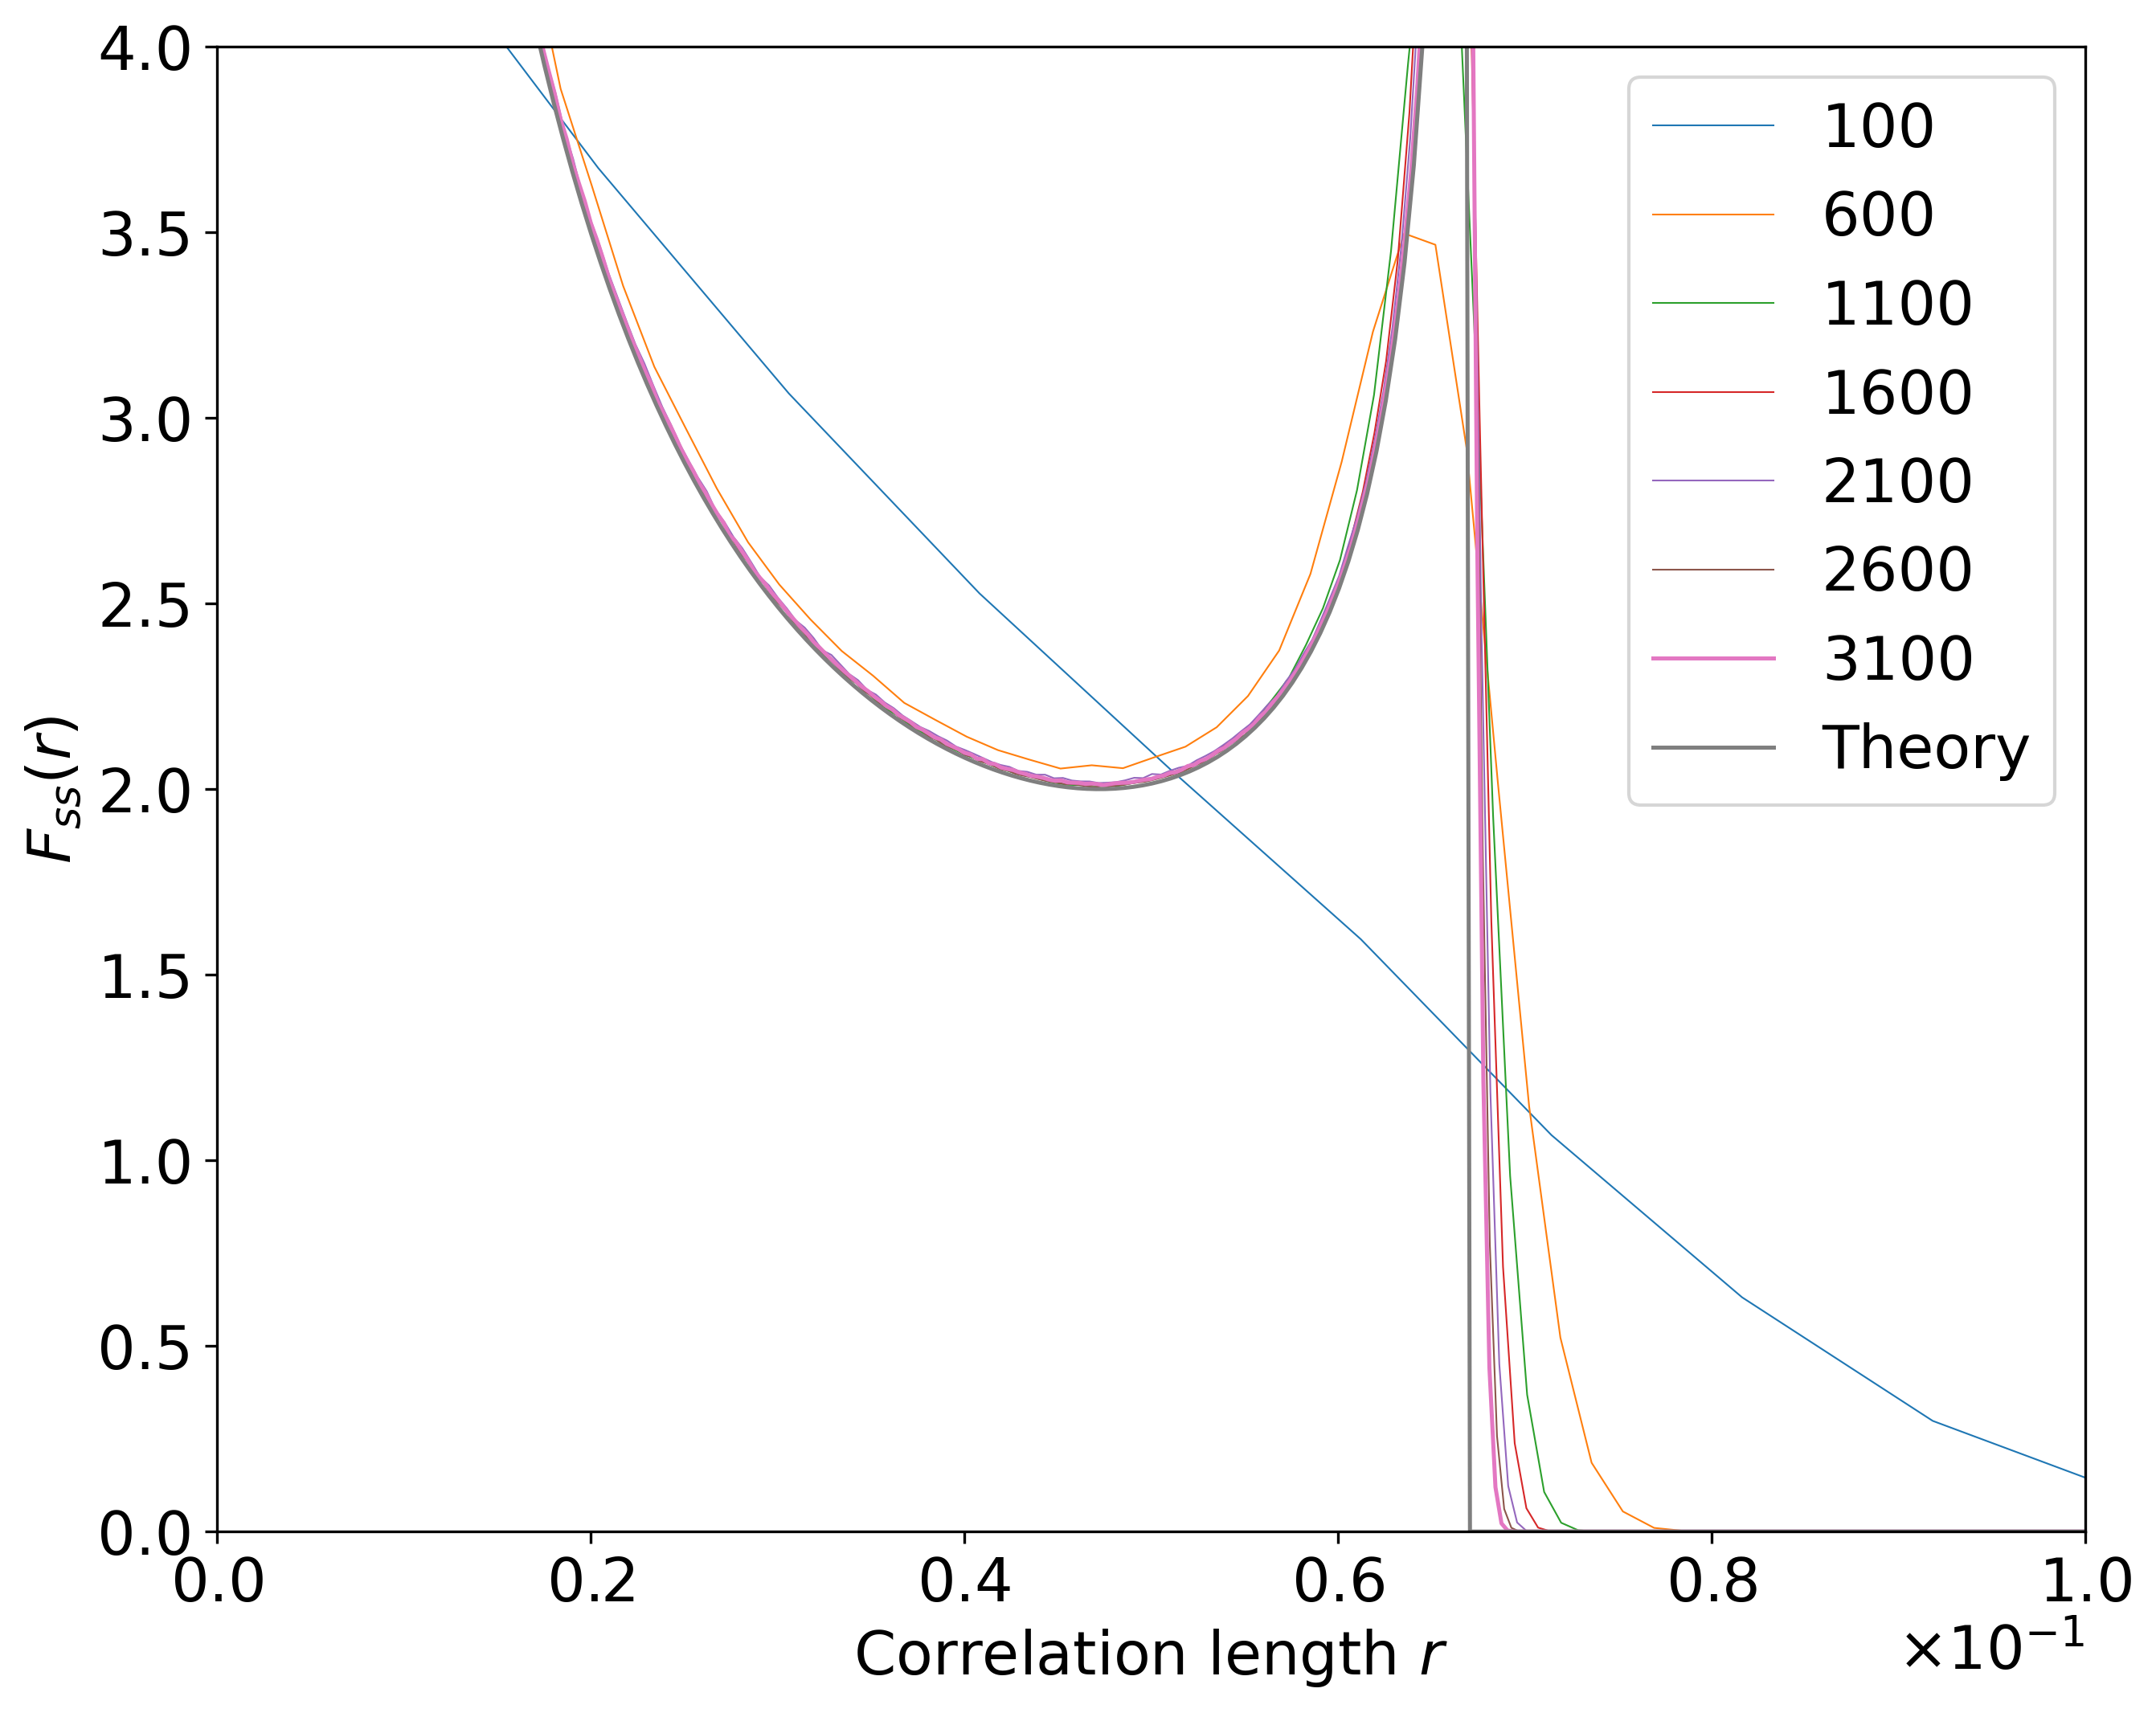
\includegraphics[width=0.45\linewidth]{images/fss-disk-7x7.png}
    \label{fig:fss-disk-5x5}}
  \caption[]{Plot of surface-surface function for a disk with radius
    $R = 0.0334$. Resolution of the image varies from $100\times 100$ pixels to
    $3100\times 3100$.}
  \label{fig:fss-disk}
\end{figure*}

If $\bm{x} \in \mathbb{R}^3$ then an inequation $f(\bm{x}) \le R^2$ defines a
ball. In this case we provide a comparison (\cref{fig:fsss-ball}) of the
algorithm in \cref{sec:algo} with the precise algorithm in
\cref{sec:fsss-3d}. There is no known analytical solution for 3D ball (one could
derive a solution in analogy with 2D case \cite{Torquato_book}, but this is
beyond the scope of the current work).
\begin{figure*}[!hpt]
  \centering
  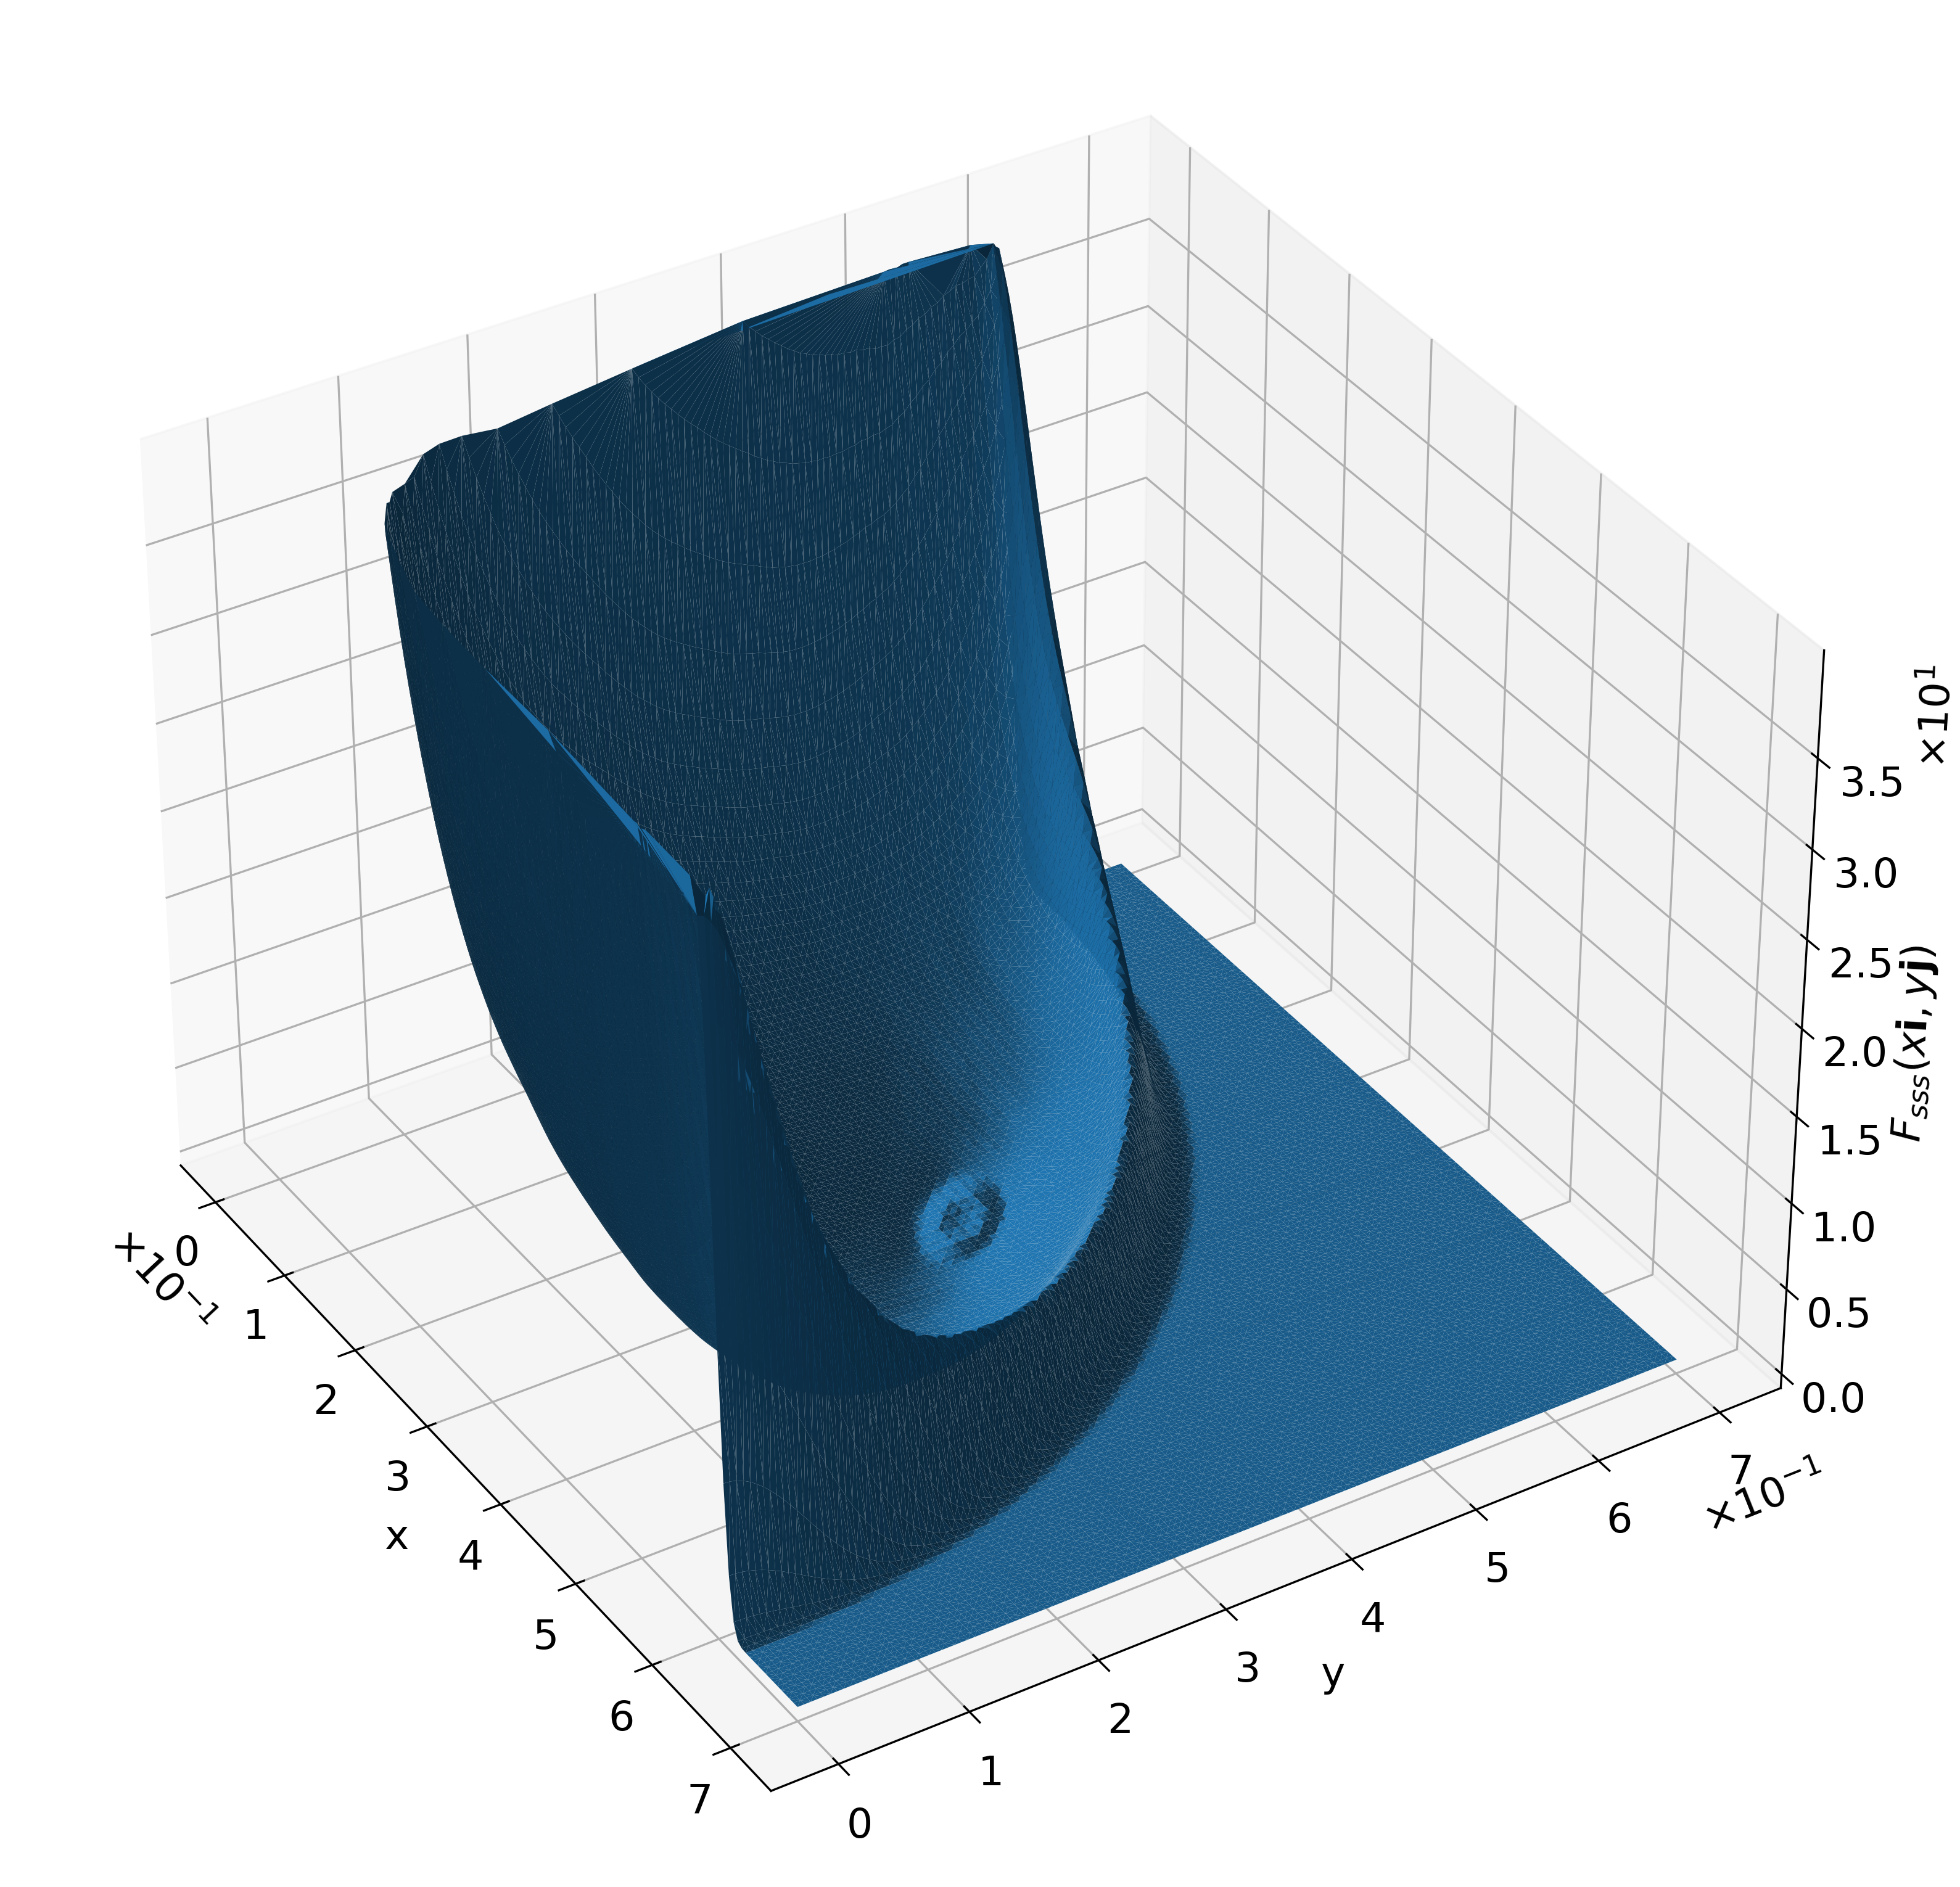
\includegraphics[width=0.45\linewidth]{images/ball-sss.png}
  \hfill
  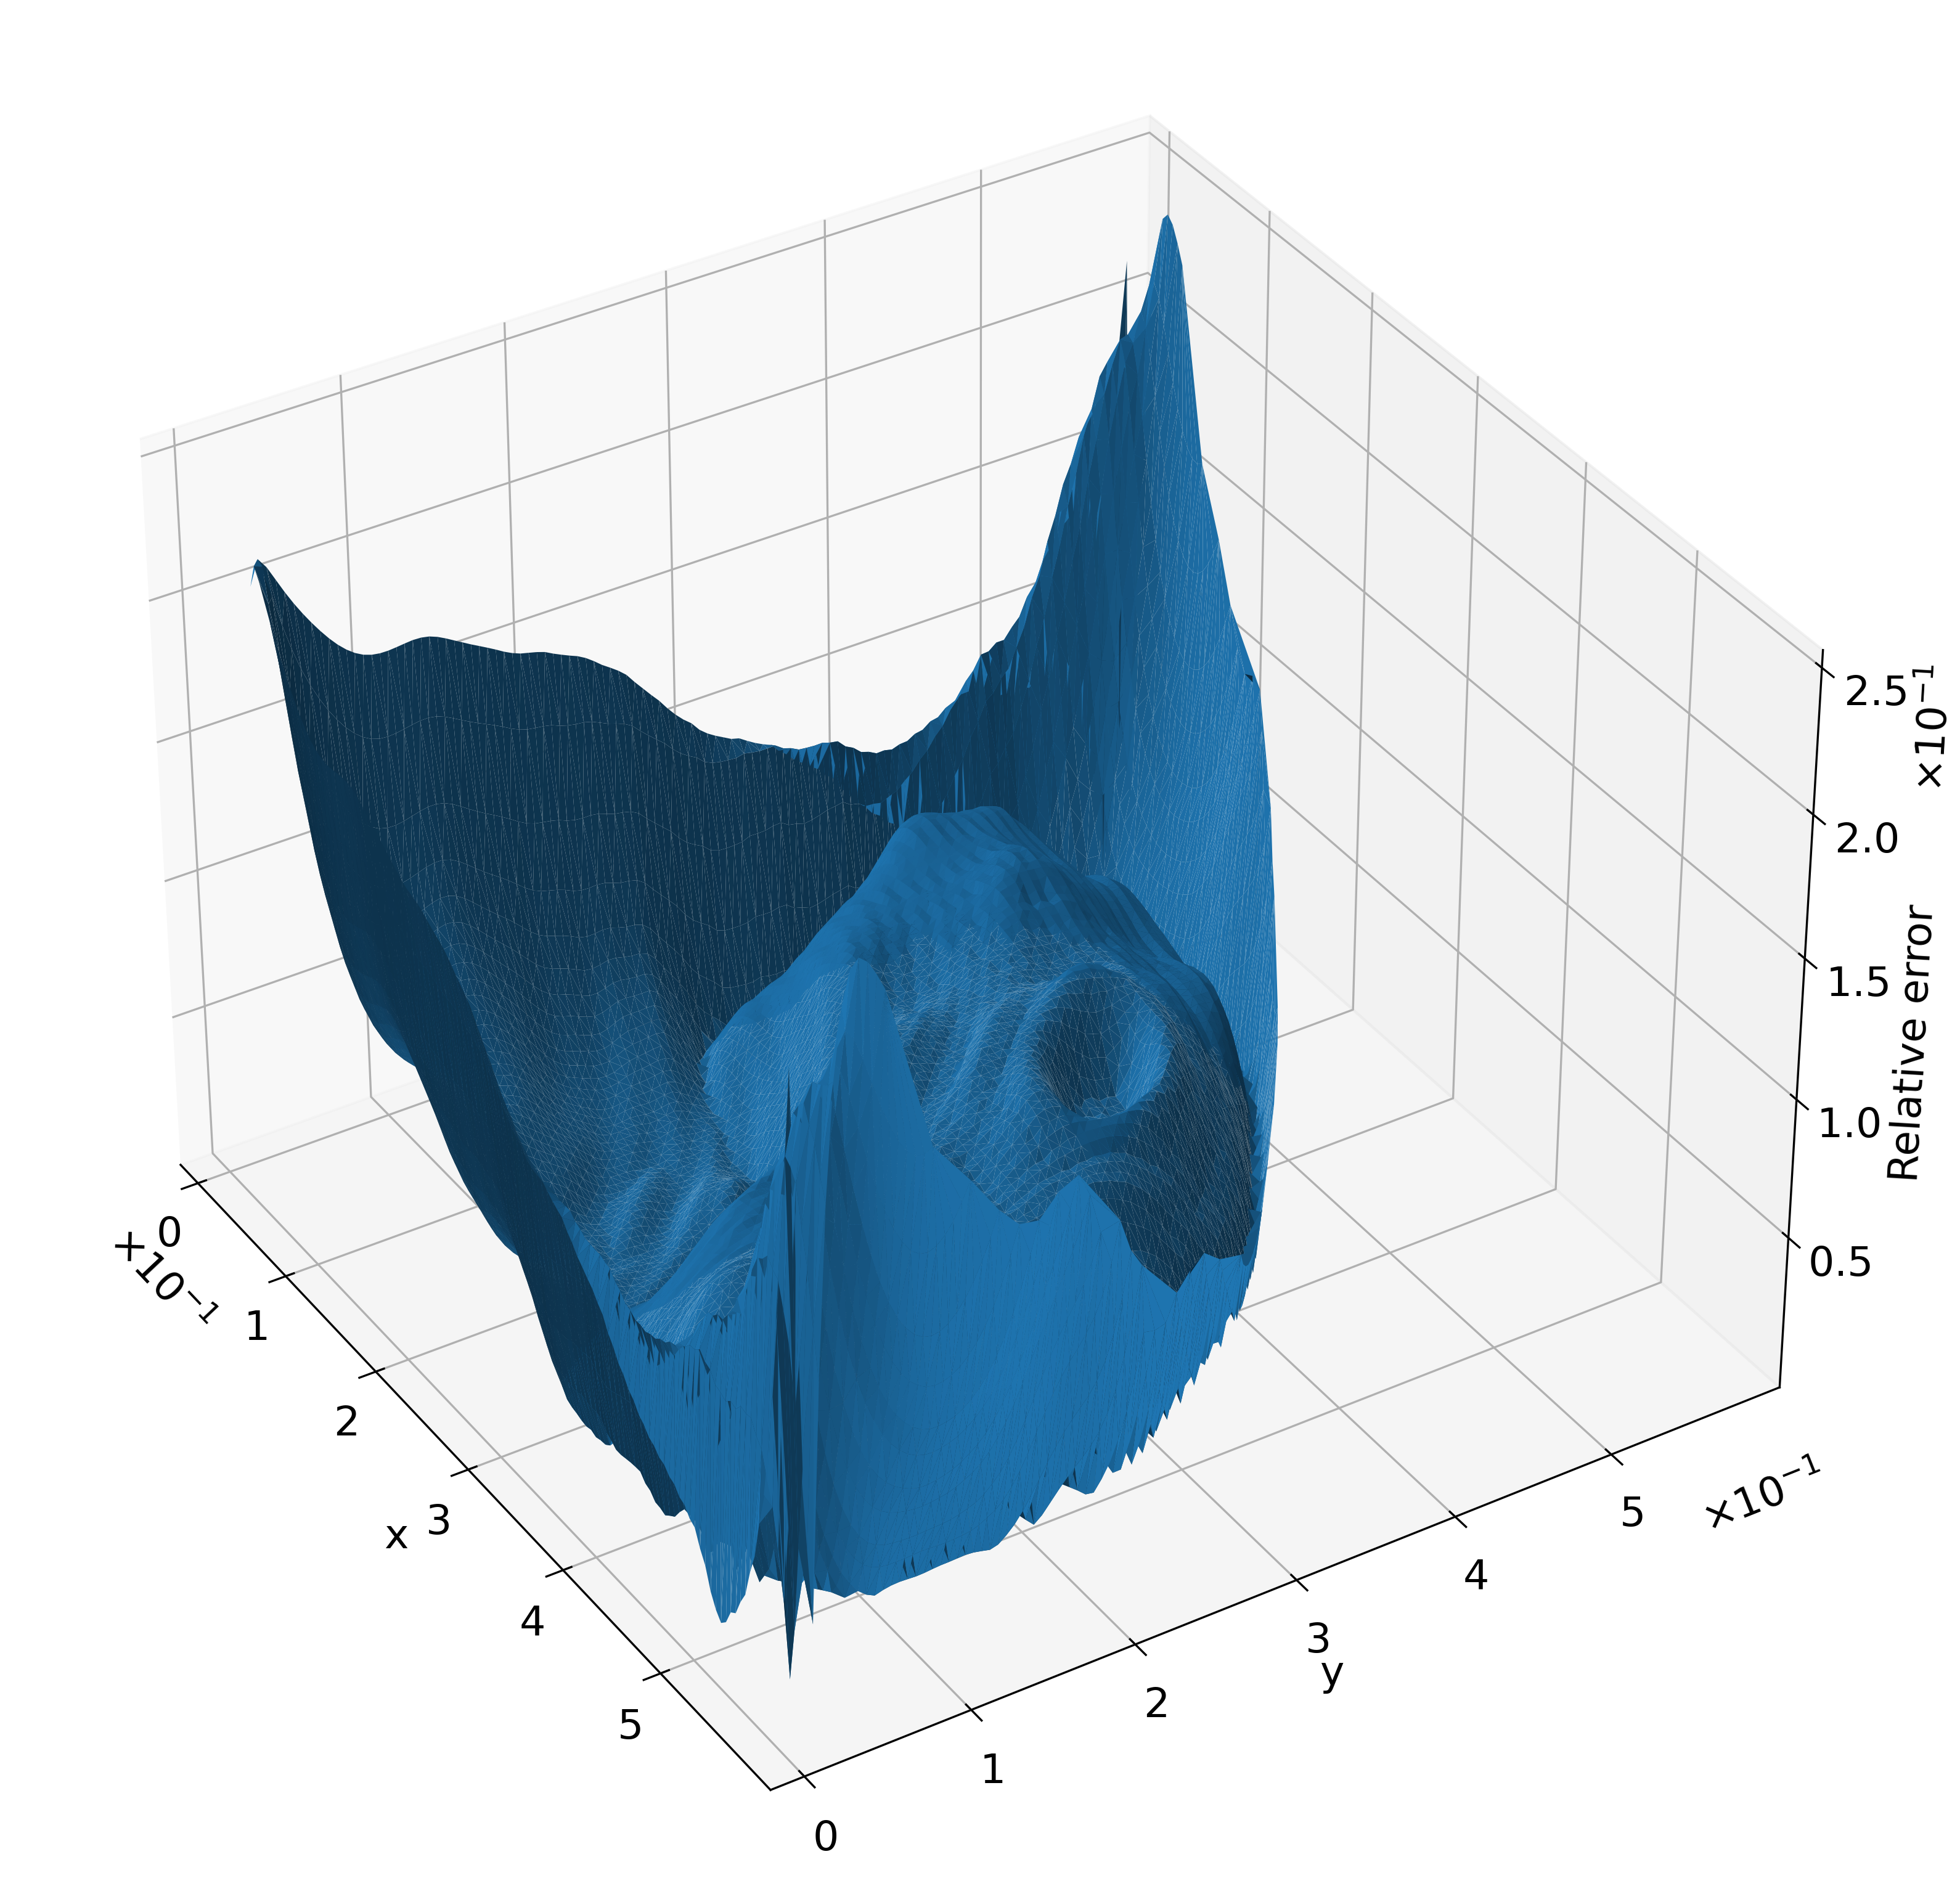
\includegraphics[width=0.45\linewidth]{images/ball-sss-error.png}
  \caption[]{On the left: Plot of $F_{sss}(\bm{r_1}, \bm{r_2})$ function
    obtained by algorithm \cref{sec:algo} for a ball with radius
    $R = 0.3$. $\bm{r_1}$ is parallel to a vector $\bm{i} = (1, 0, 0)$ and
    $\bm{r_2}$ is parallel to a vector $\bm{j} = (0, 1, 0)$. Vectors $\bm{i}$
    and $\bm{j}$ constitute a two-dimensional parameter space for $F_{sss}$. On
    the right: Relative error of computation. True values for $F_{sss}$ are
    obtained by algorithm in \cref{sec:fsss-3d}.}
  \label{fig:fsss-ball}
\end{figure*}

We conclude that if a theoretical solution is known for the correlation function
$F_{ss}$ or $F_{sss}$, then evaluation of this function using our continuous
approach does not differ from this theoretical solution if all crossings of
the interface with its translated self are found correctly (which is the case
for all sets described in this paper). This approach can be used to assess the
quality of the algorithm for discretized sets. As expected, performance of the
latter depends on the image resolution and the choise of an edge detection
filter (the new filter $H'$ is preferable than $H$ for images with good
resolution, see \cref{sec:influence}).

\subsection{Gaussian mixture}
\label{sec:gauss}
\begin{figure*}[!hpt]
  \centering
  \subfigure[An example of a ``blob'' generated by Gaussian mixture $f(x,y)$
    which consists of four Gaussian functions. White area is where
    $f(x,y) \le 3$.] {
    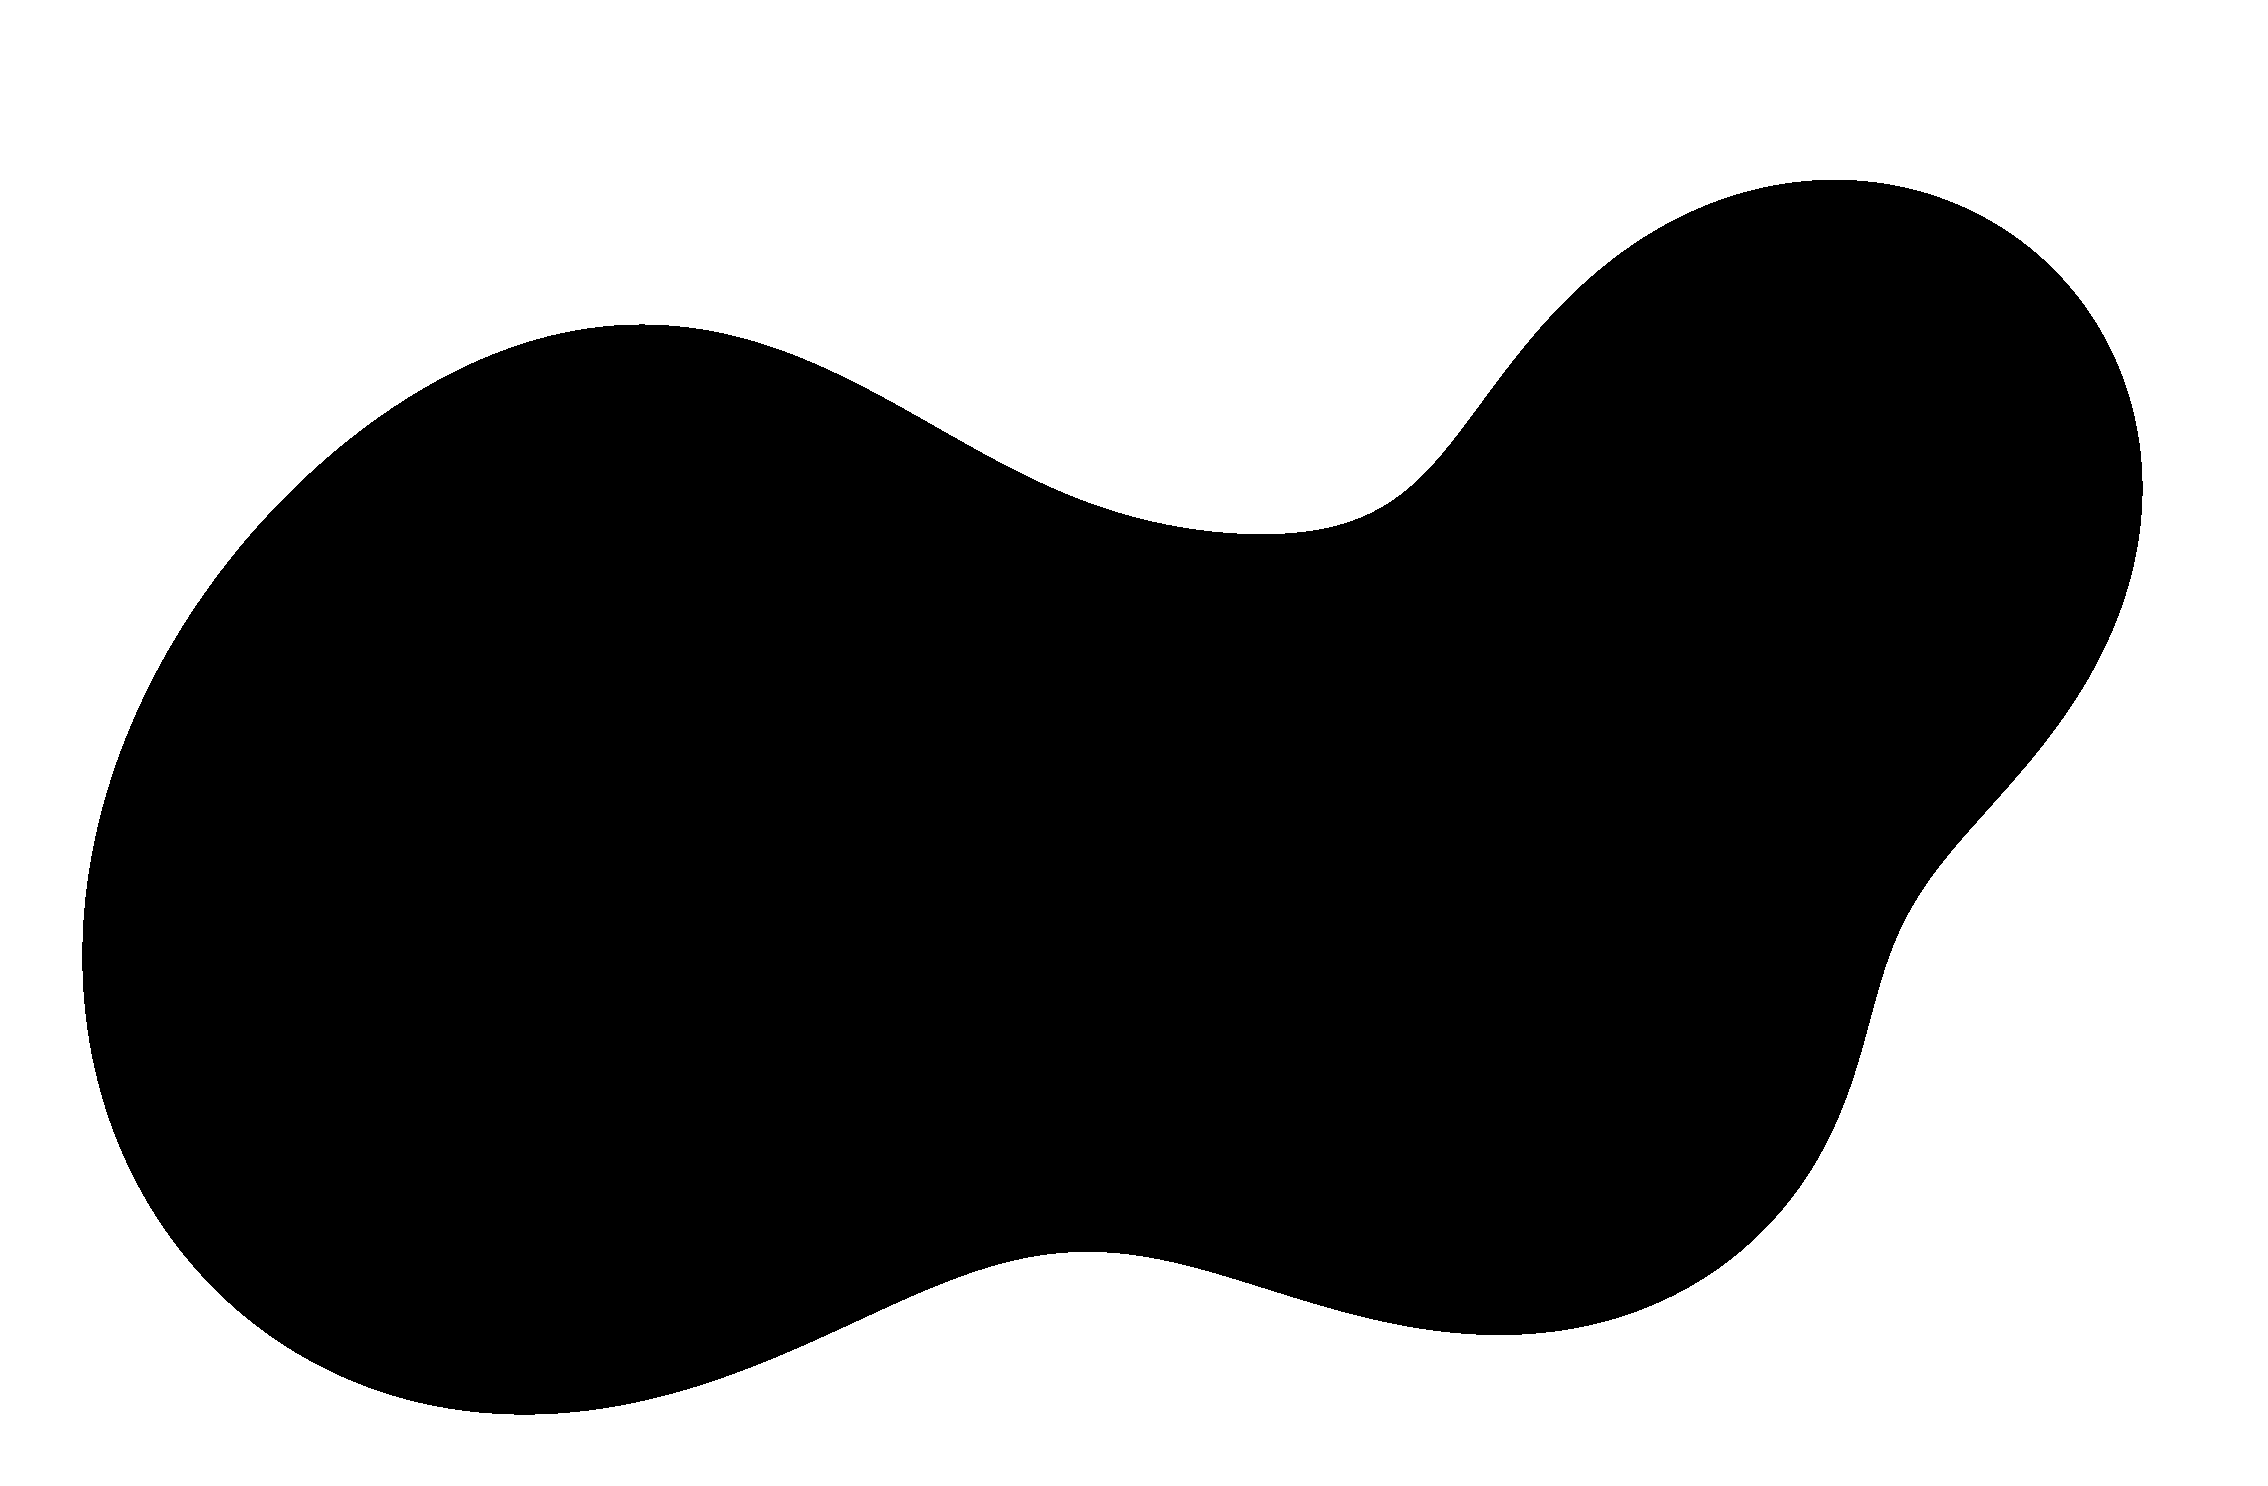
\includegraphics[width=0.45\linewidth, frame]{images/blob.png}
    \label{fig:blob}}
  \hfill
  \subfigure[An example of generated ellipses.] {
    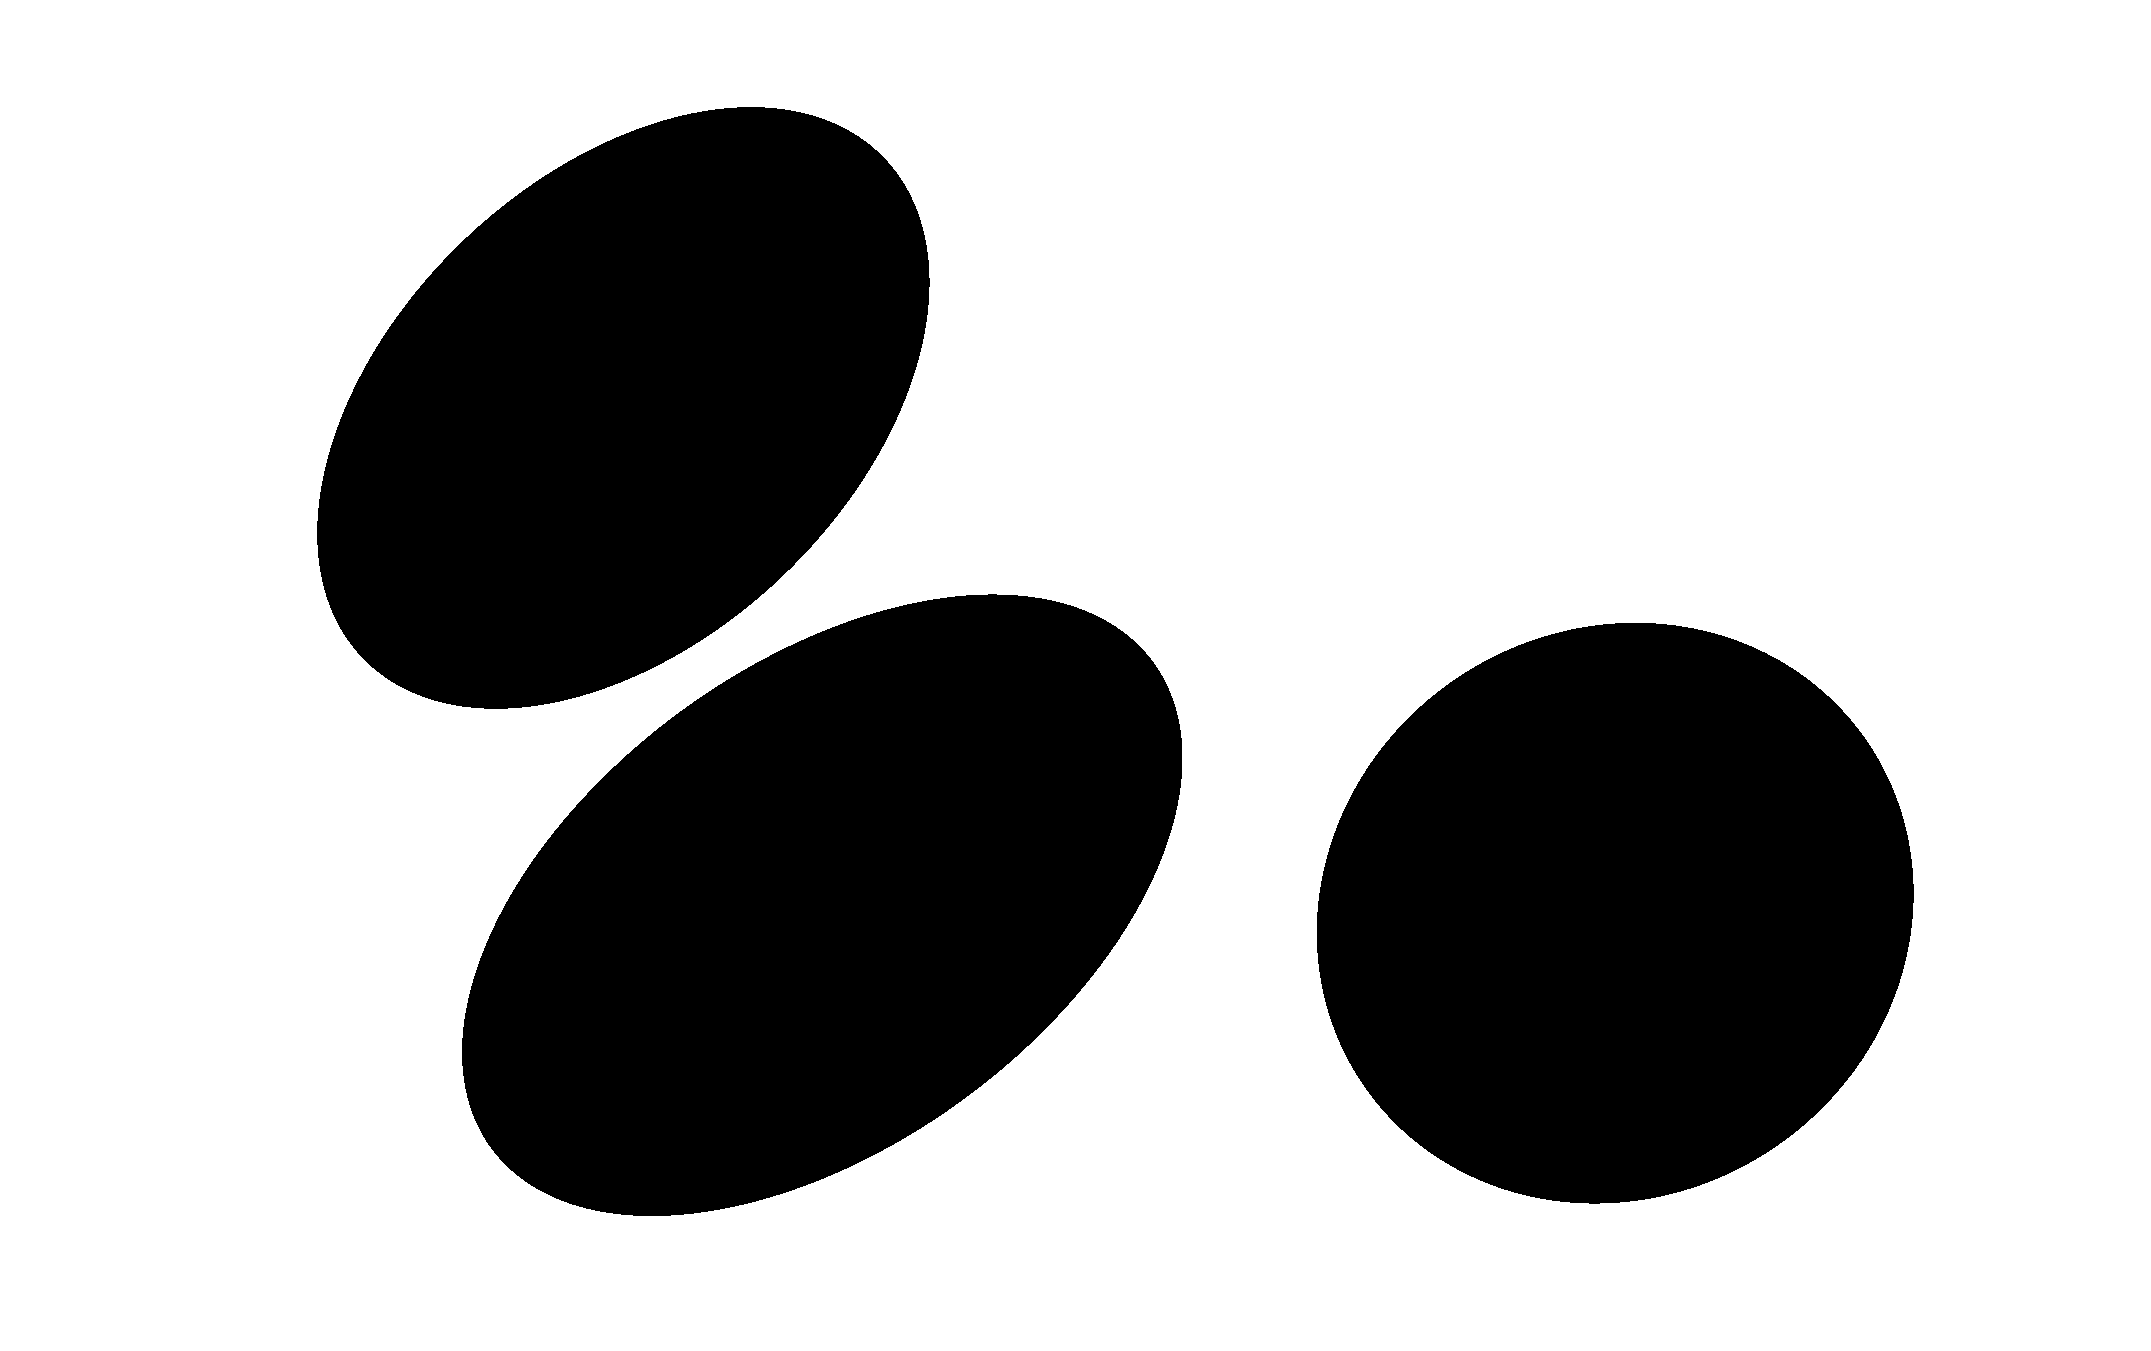
\includegraphics[width=0.45\linewidth, frame]{images/ellipses.png}
    \label{fig:ellipses}}
  \caption[]{Examples of sets with smooth boundary.}
\end{figure*}
Let us now consider more complex surfaces, including concave shapes. Take $N$
random values of each of $a_i$, $b_i$ and $\sigma_i$. Let $f$ be:
\begin{equation}
  f(x,y) = \sum_{i=1}^N \frac{1}{\sigma_i} \exp(\frac{-(x-a_i)^2-(y-b_i)^2}{\sigma_i^2})
\end{equation}
Inequality $f(x,y) \le T$ defines a ``blob'' like one which can be seen on
\cref{fig:blob}. We can use the algorithm developed in \cref{sec:fss-2d} to
compute precise values of $F_{ss}$ for this blob and compare them with values
obtained by using the algorithm in section \cref{sec:algo}. The result of this
comparison is presented on \cref{fig:fss-blob}.
\begin{figure*}[!hpt]
  \centering
  \subfigure[$3\times 3$ kernel $H$]{
    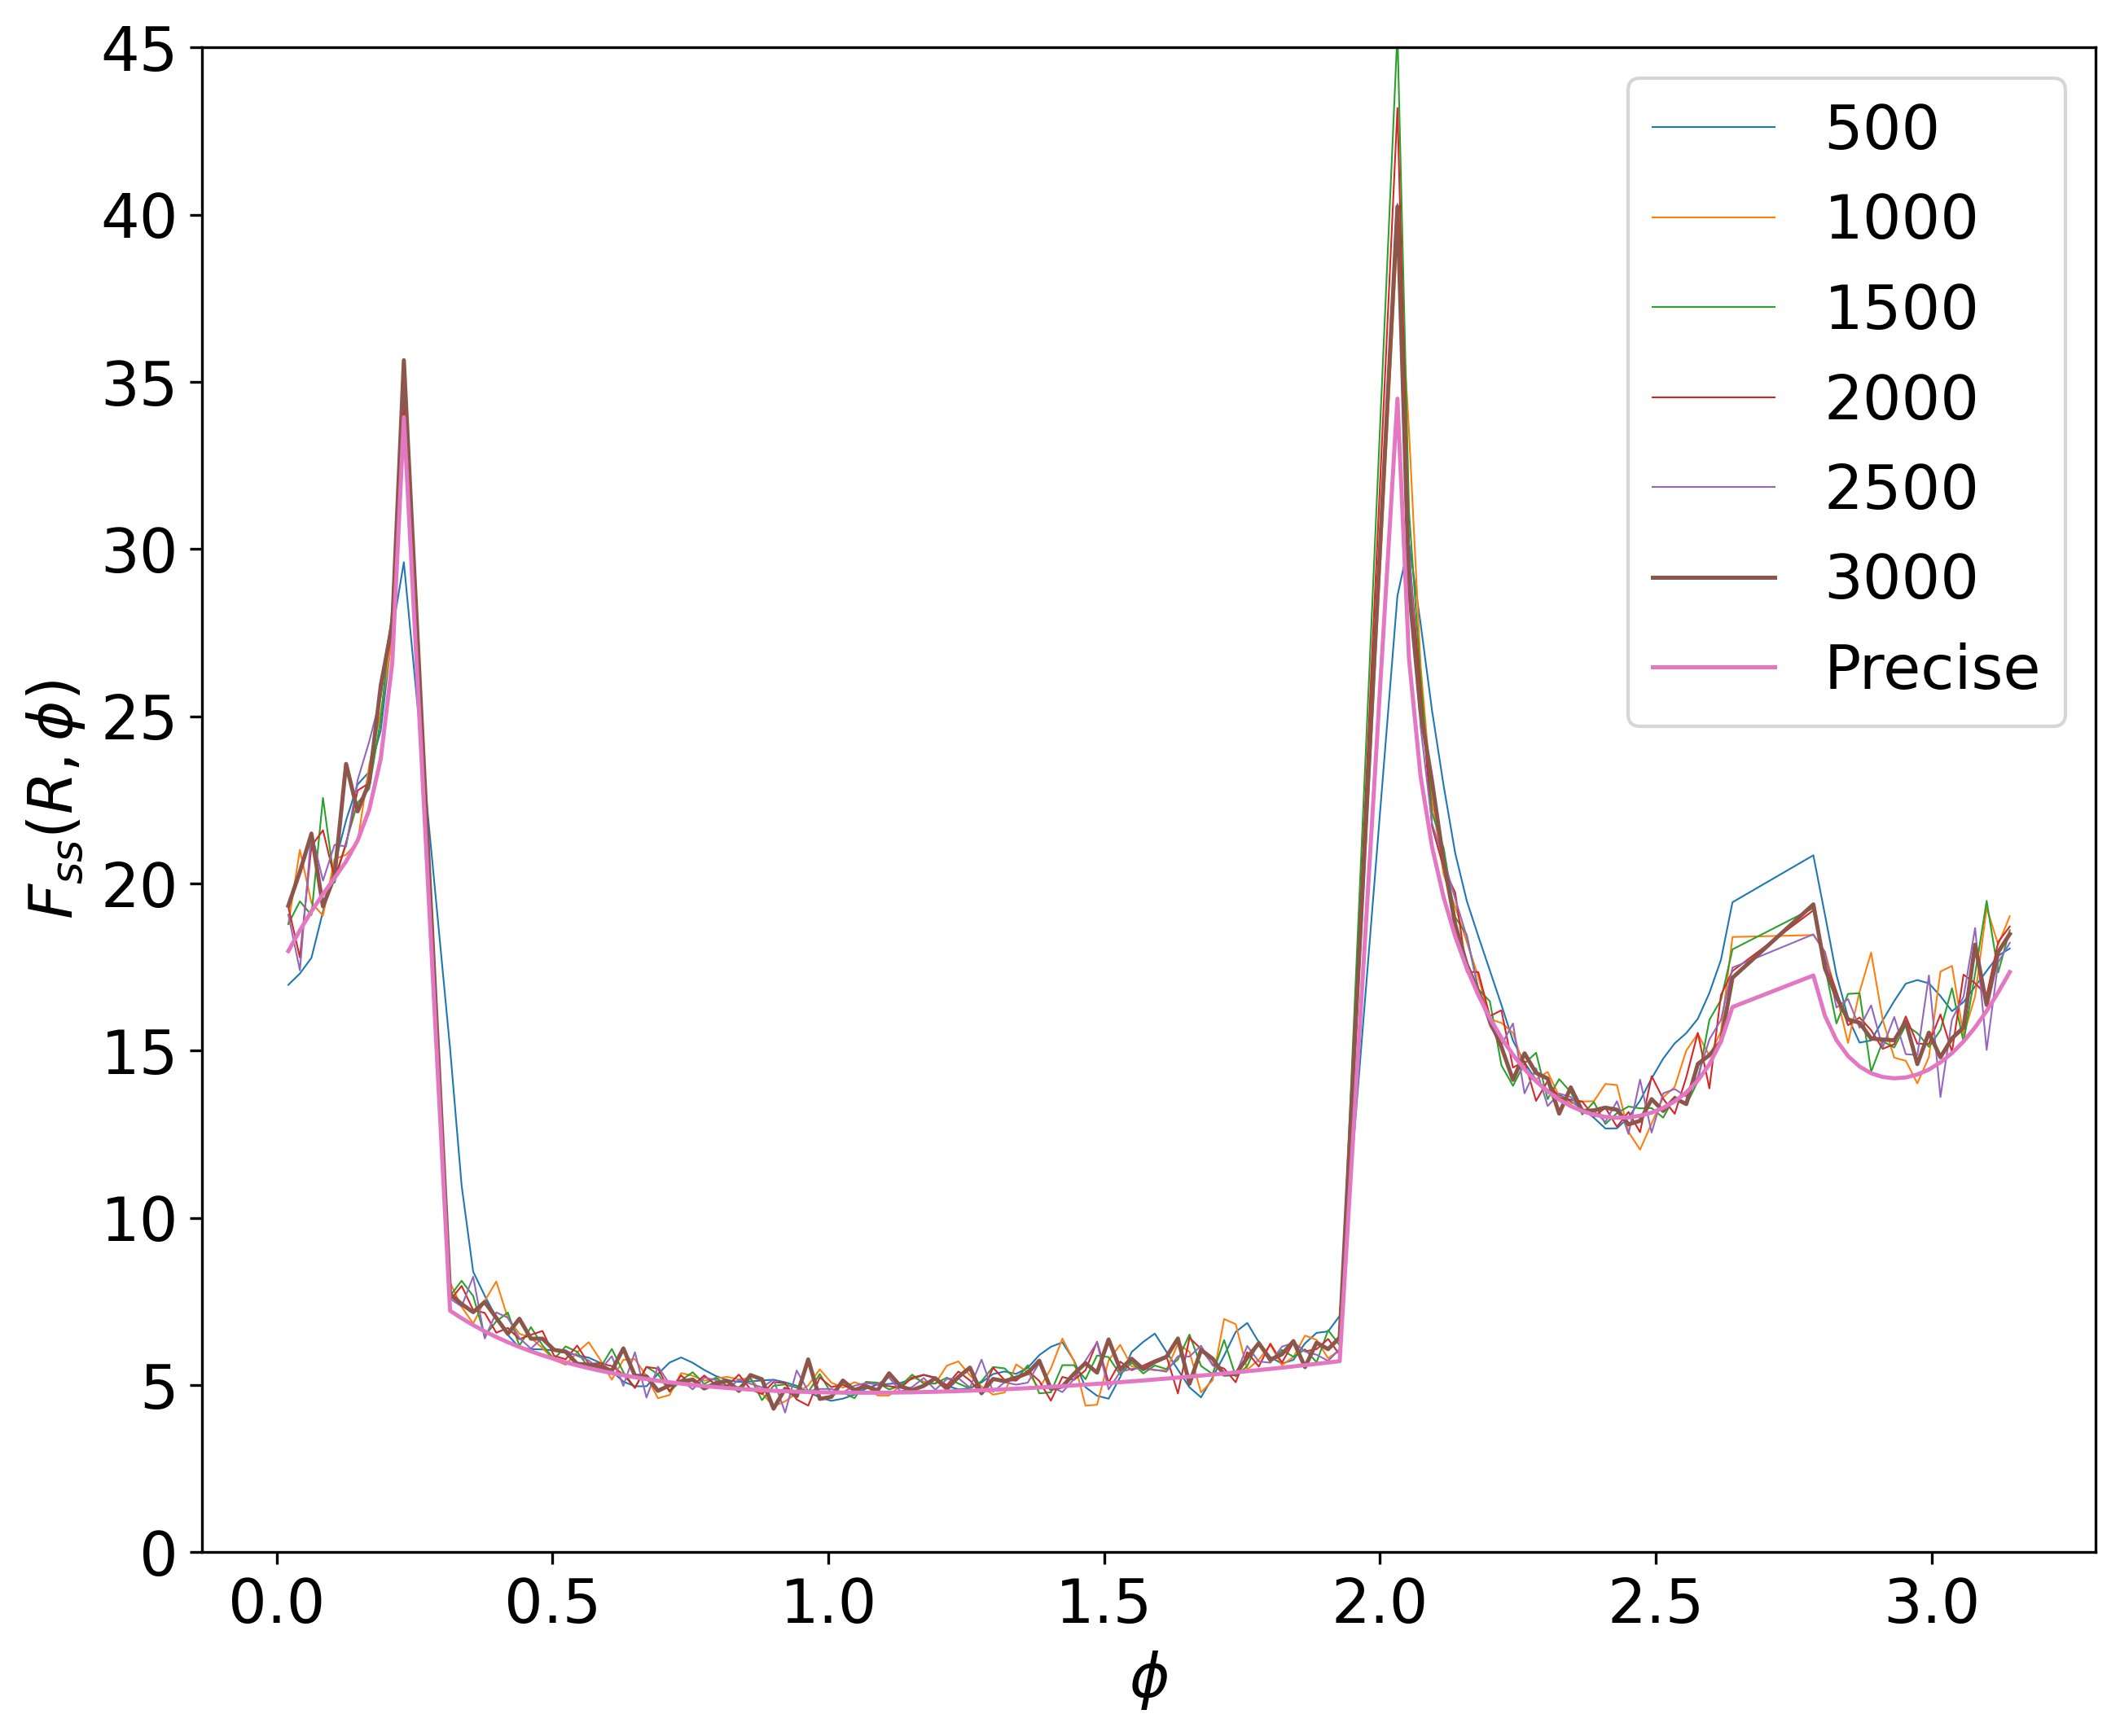
\includegraphics[width=0.45\linewidth]{images/fss-blob-3x3.png}
    \label{fig:fss-blob-3x3}}
  \hfill
  \subfigure[$7\times 7$ kernel $H'$]{
    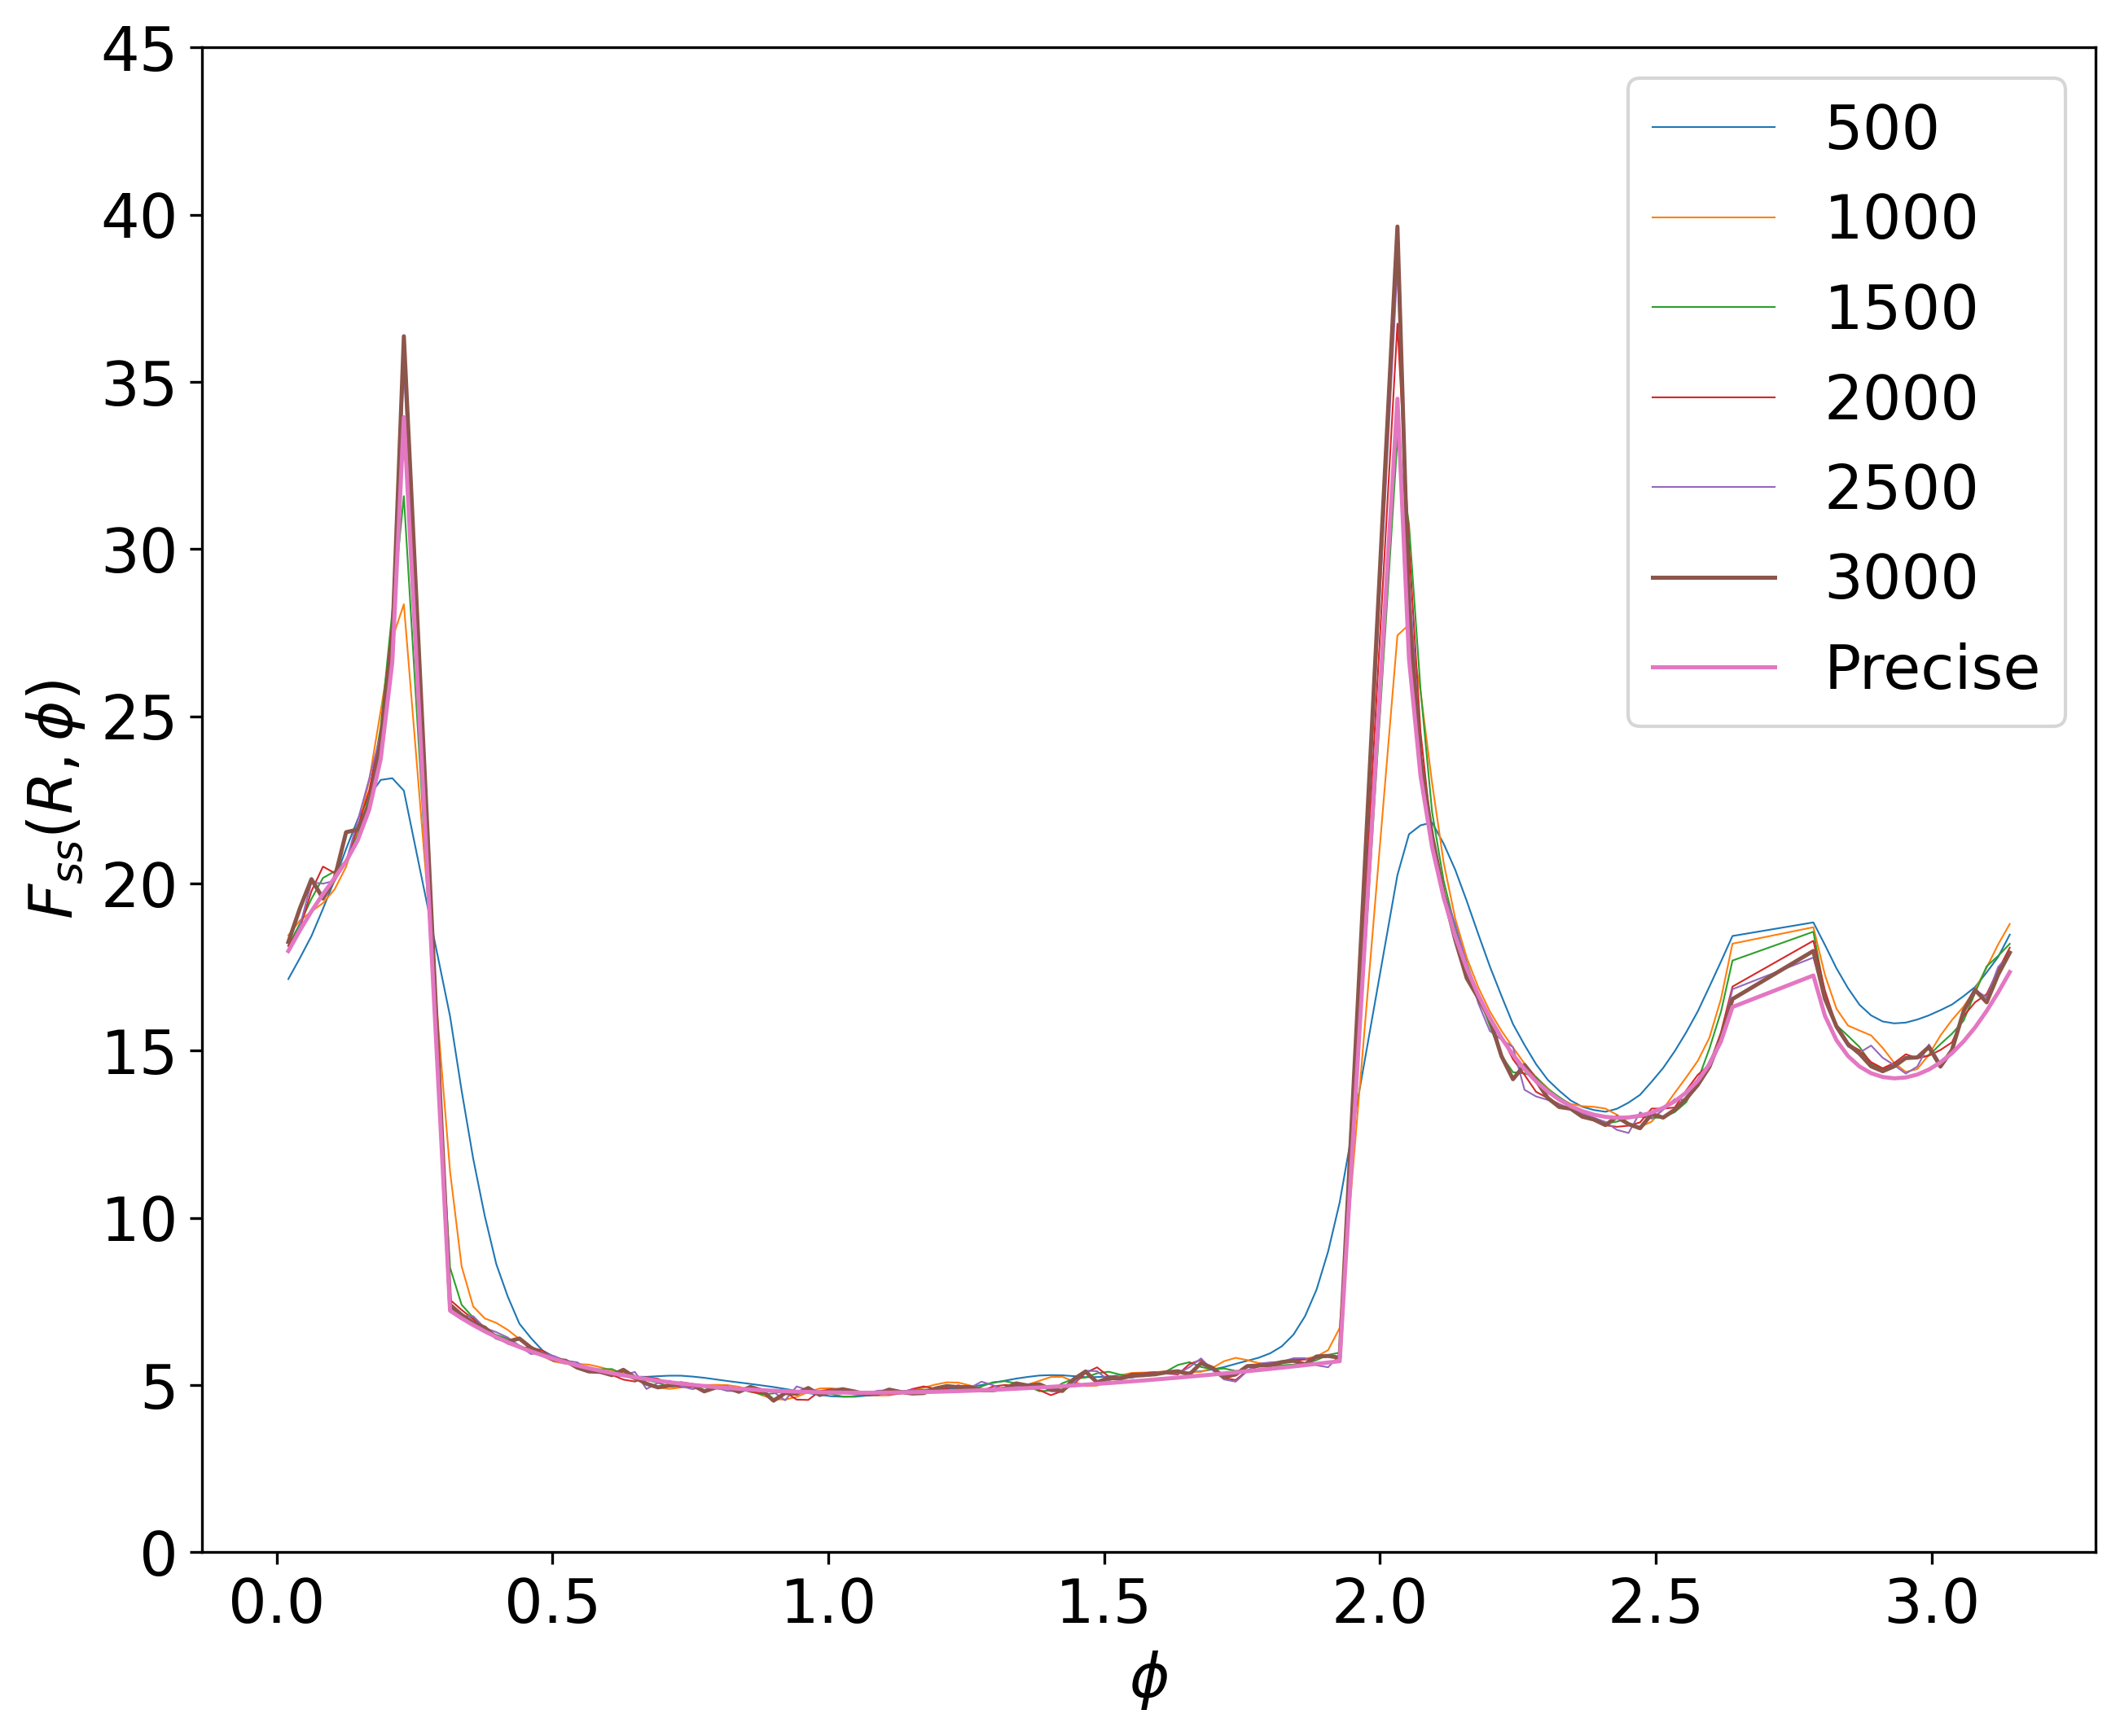
\includegraphics[width=0.45\linewidth]{images/fss-blob-7x7.png}
    \label{fig:fss-blob-5x5}}
  \caption[]{Plot of the surface-surface function for the blob on
    \cref{fig:blob}. Values of $F_{ss}$ were calculated in semi-circle with
    radius $R = 0.3$ and angle $\phi$ varying from $0$ to $\pi$. Resolution of
    the image varies from $500\times 500$ pixels to $3000\times 3000$.}
  \label{fig:fss-blob}
\end{figure*}

\subsection{Ellipses}
\label{sec:ellipses}
Take $N$ random values $a_i$, $b_i$, $c_i$, $x^c_i$ and $y^c_i$ and define
\begin{equation}
  f_i(x, y) = a_i(x-x^c_i)^2 + b(x-x^c_i)(y-y^c_i) + c_i(y-y^c_i)^2
\end{equation}
with $a_ic_i - b_i^2 > 0$. Inequation
\begin{equation}
  \min_i f_i(x, y) < A^2
\end{equation}
defines $N$ ellipses like those which can be seen on \cref{fig:ellipses}. A
comparison between two algorithms is on \cref{fig:fss-ellipses}.
\begin{figure*}[!hpt]
  \centering
  \subfigure[$3\times 3$ kernel $H$]{
    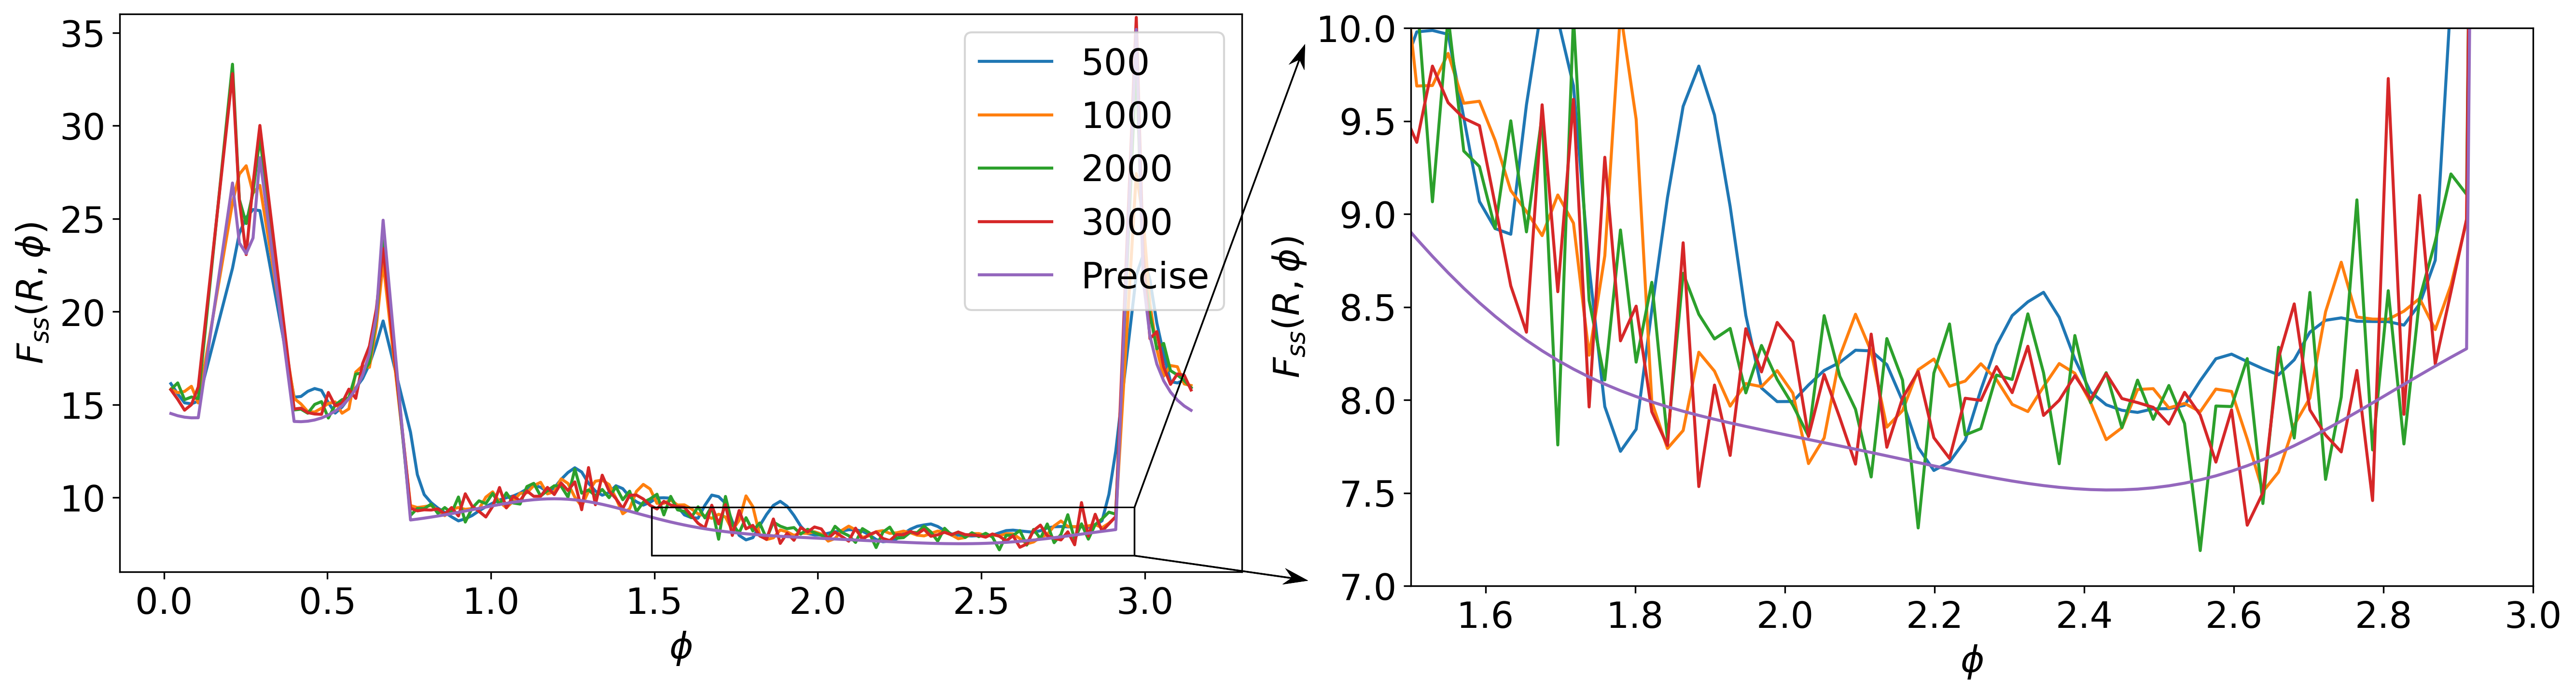
\includegraphics[width=0.45\linewidth]{images/fss-ellipses-3x3.png}
    \label{fig:fss-ellipses-3x3}}
  \hfill
  \subfigure[$7\times 7$ kernel $H'$]{
    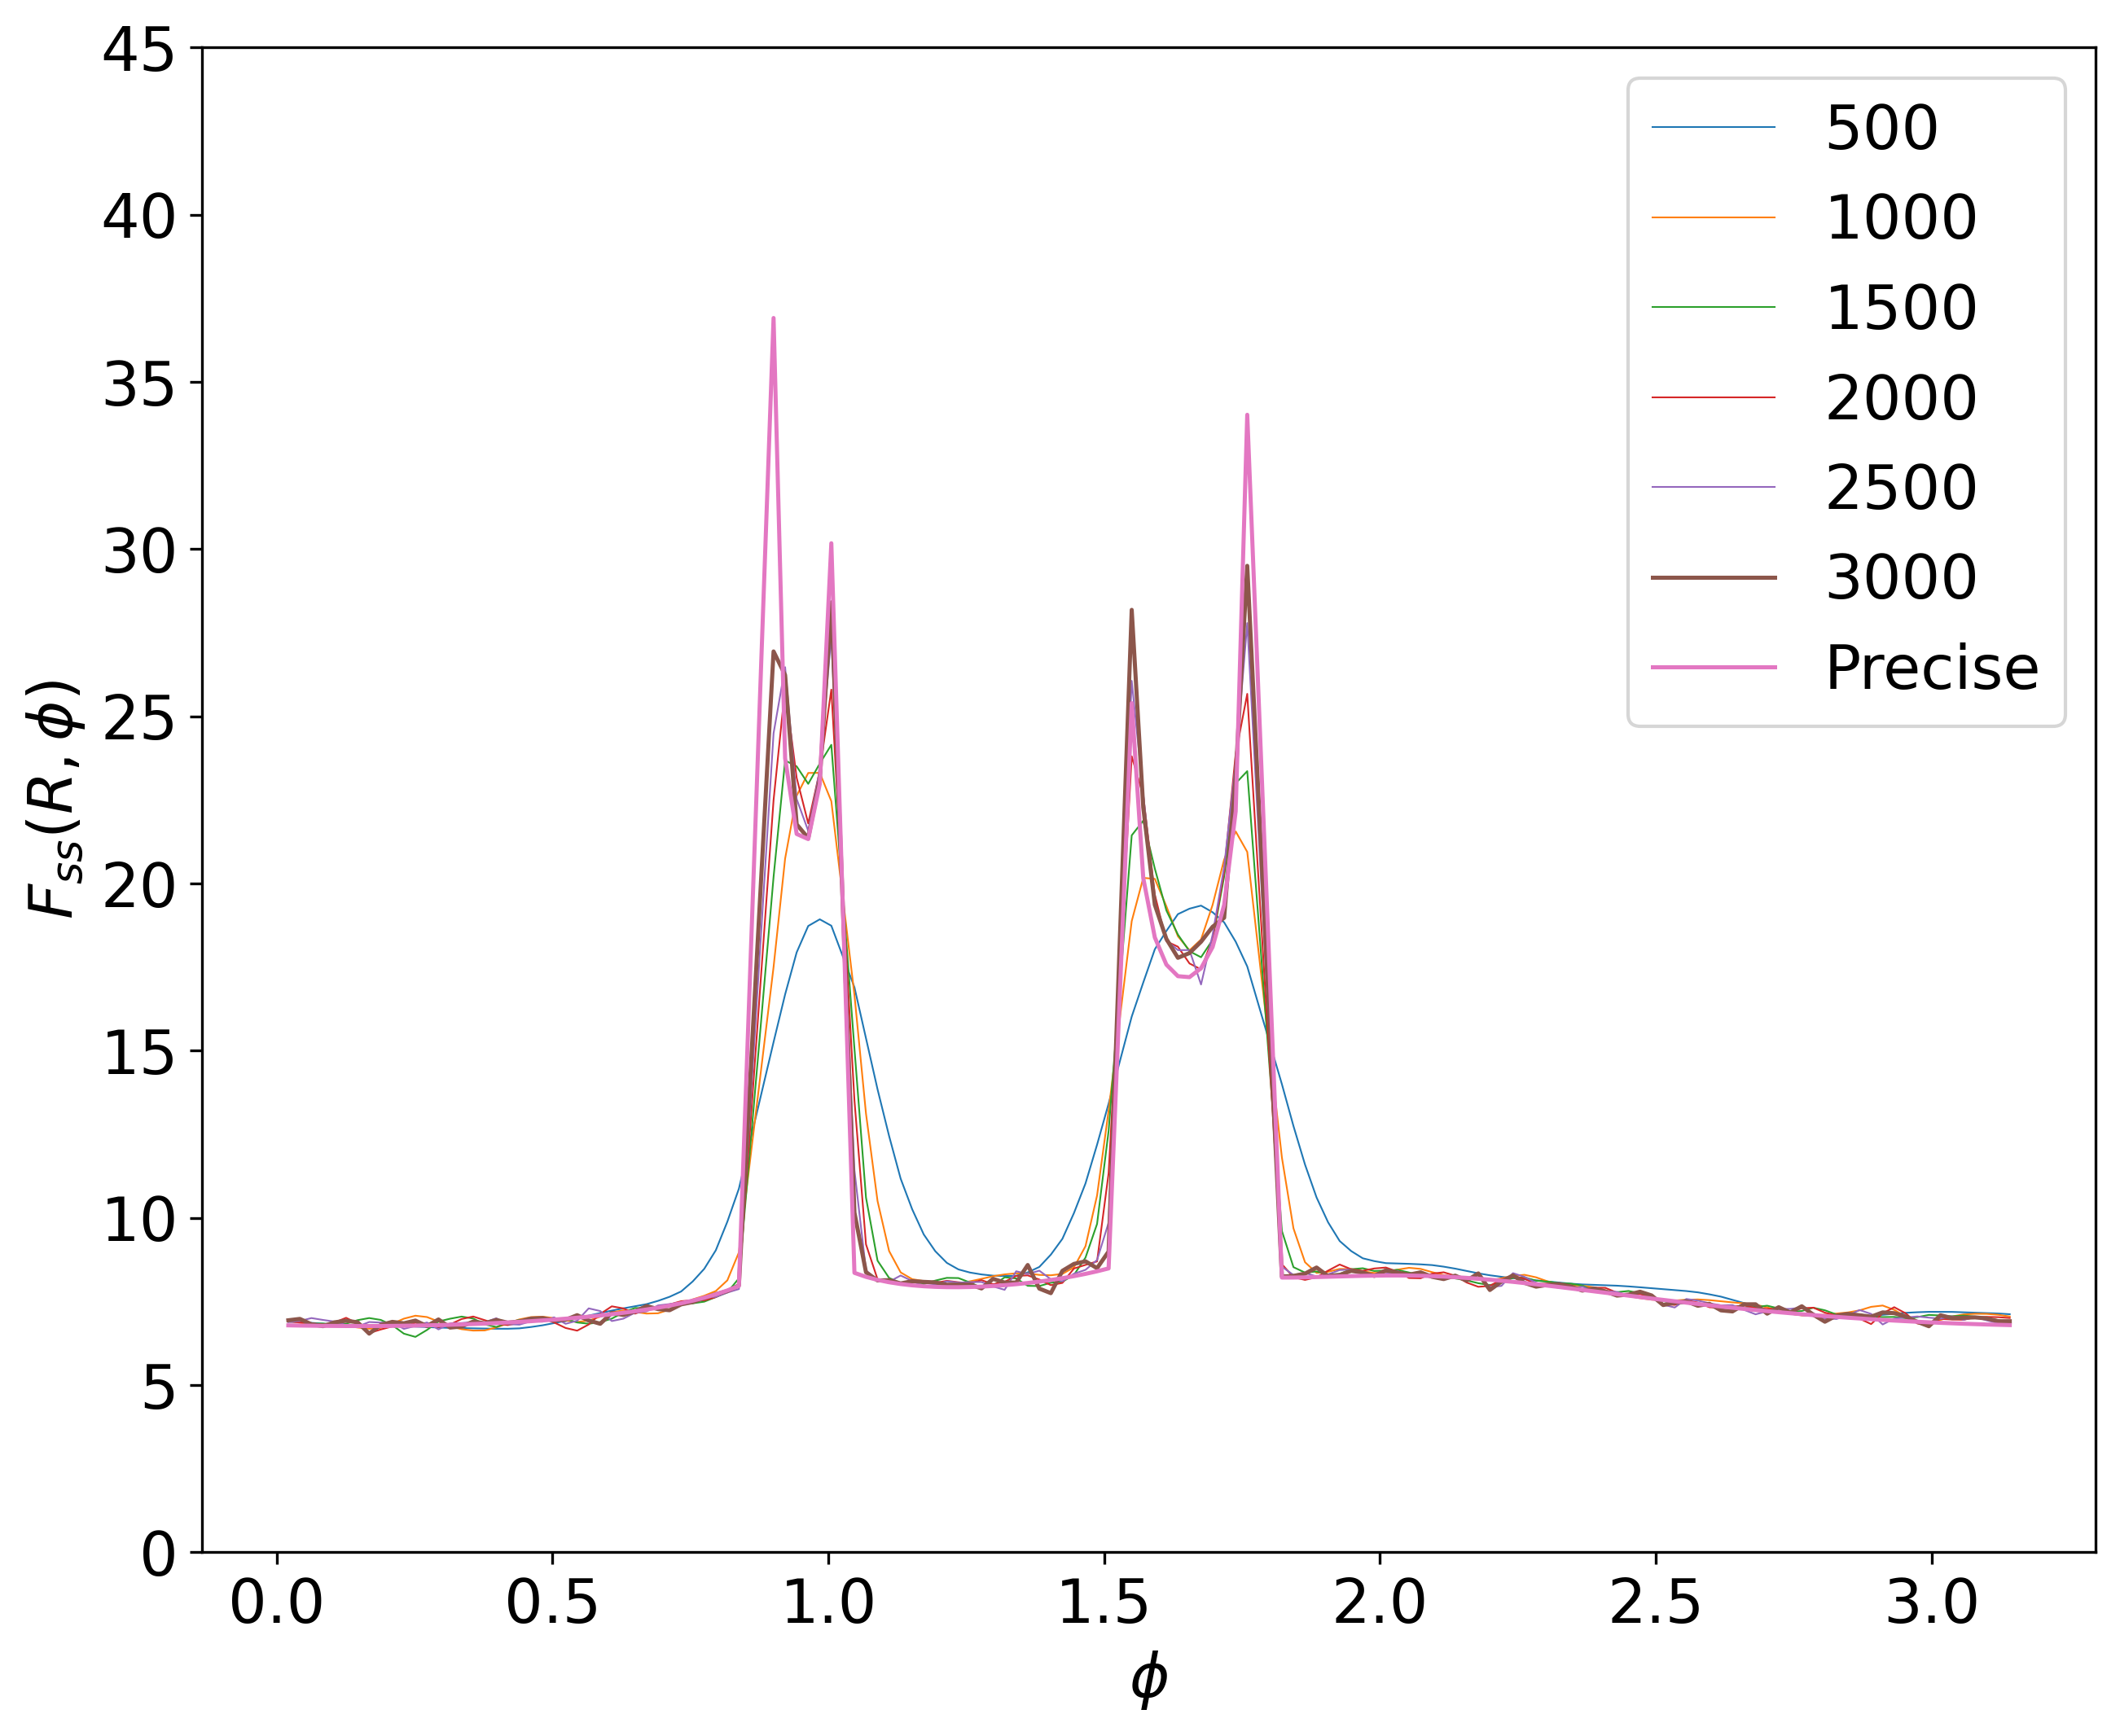
\includegraphics[width=0.45\linewidth]{images/fss-ellipses-7x7.png}
    \label{fig:fss-ellipses-5x5}}
  \caption[]{Plot of the surface-surface function for ellipses on
    \cref{fig:ellipses}. Values of $F_{ss}$ were calculated in semi-circle with
    radius $R = 0.1$ and angle $\phi$ varying from $0$ to $\pi$. Resolution of
    the image varies from $500\times 500$ pixels to $3000\times 3000$.}
  \label{fig:fss-ellipses}
\end{figure*}

Again, we observe the convergence of continuous and discrete approaches to
compute surface functions \cite{Samarin} that confirms the accuracy of results
thus obtained.

\subsection{Influence of filter $H'$ on computation accuracy}
\label{sec:influence}
\begin{figure*}[!hpt]
  \centering
  \subfigure[Surface-surface function calculated for a ball with radius
    $R = 0.24$. Image dimensions are  $450 \times 450 \times 450$.]{
    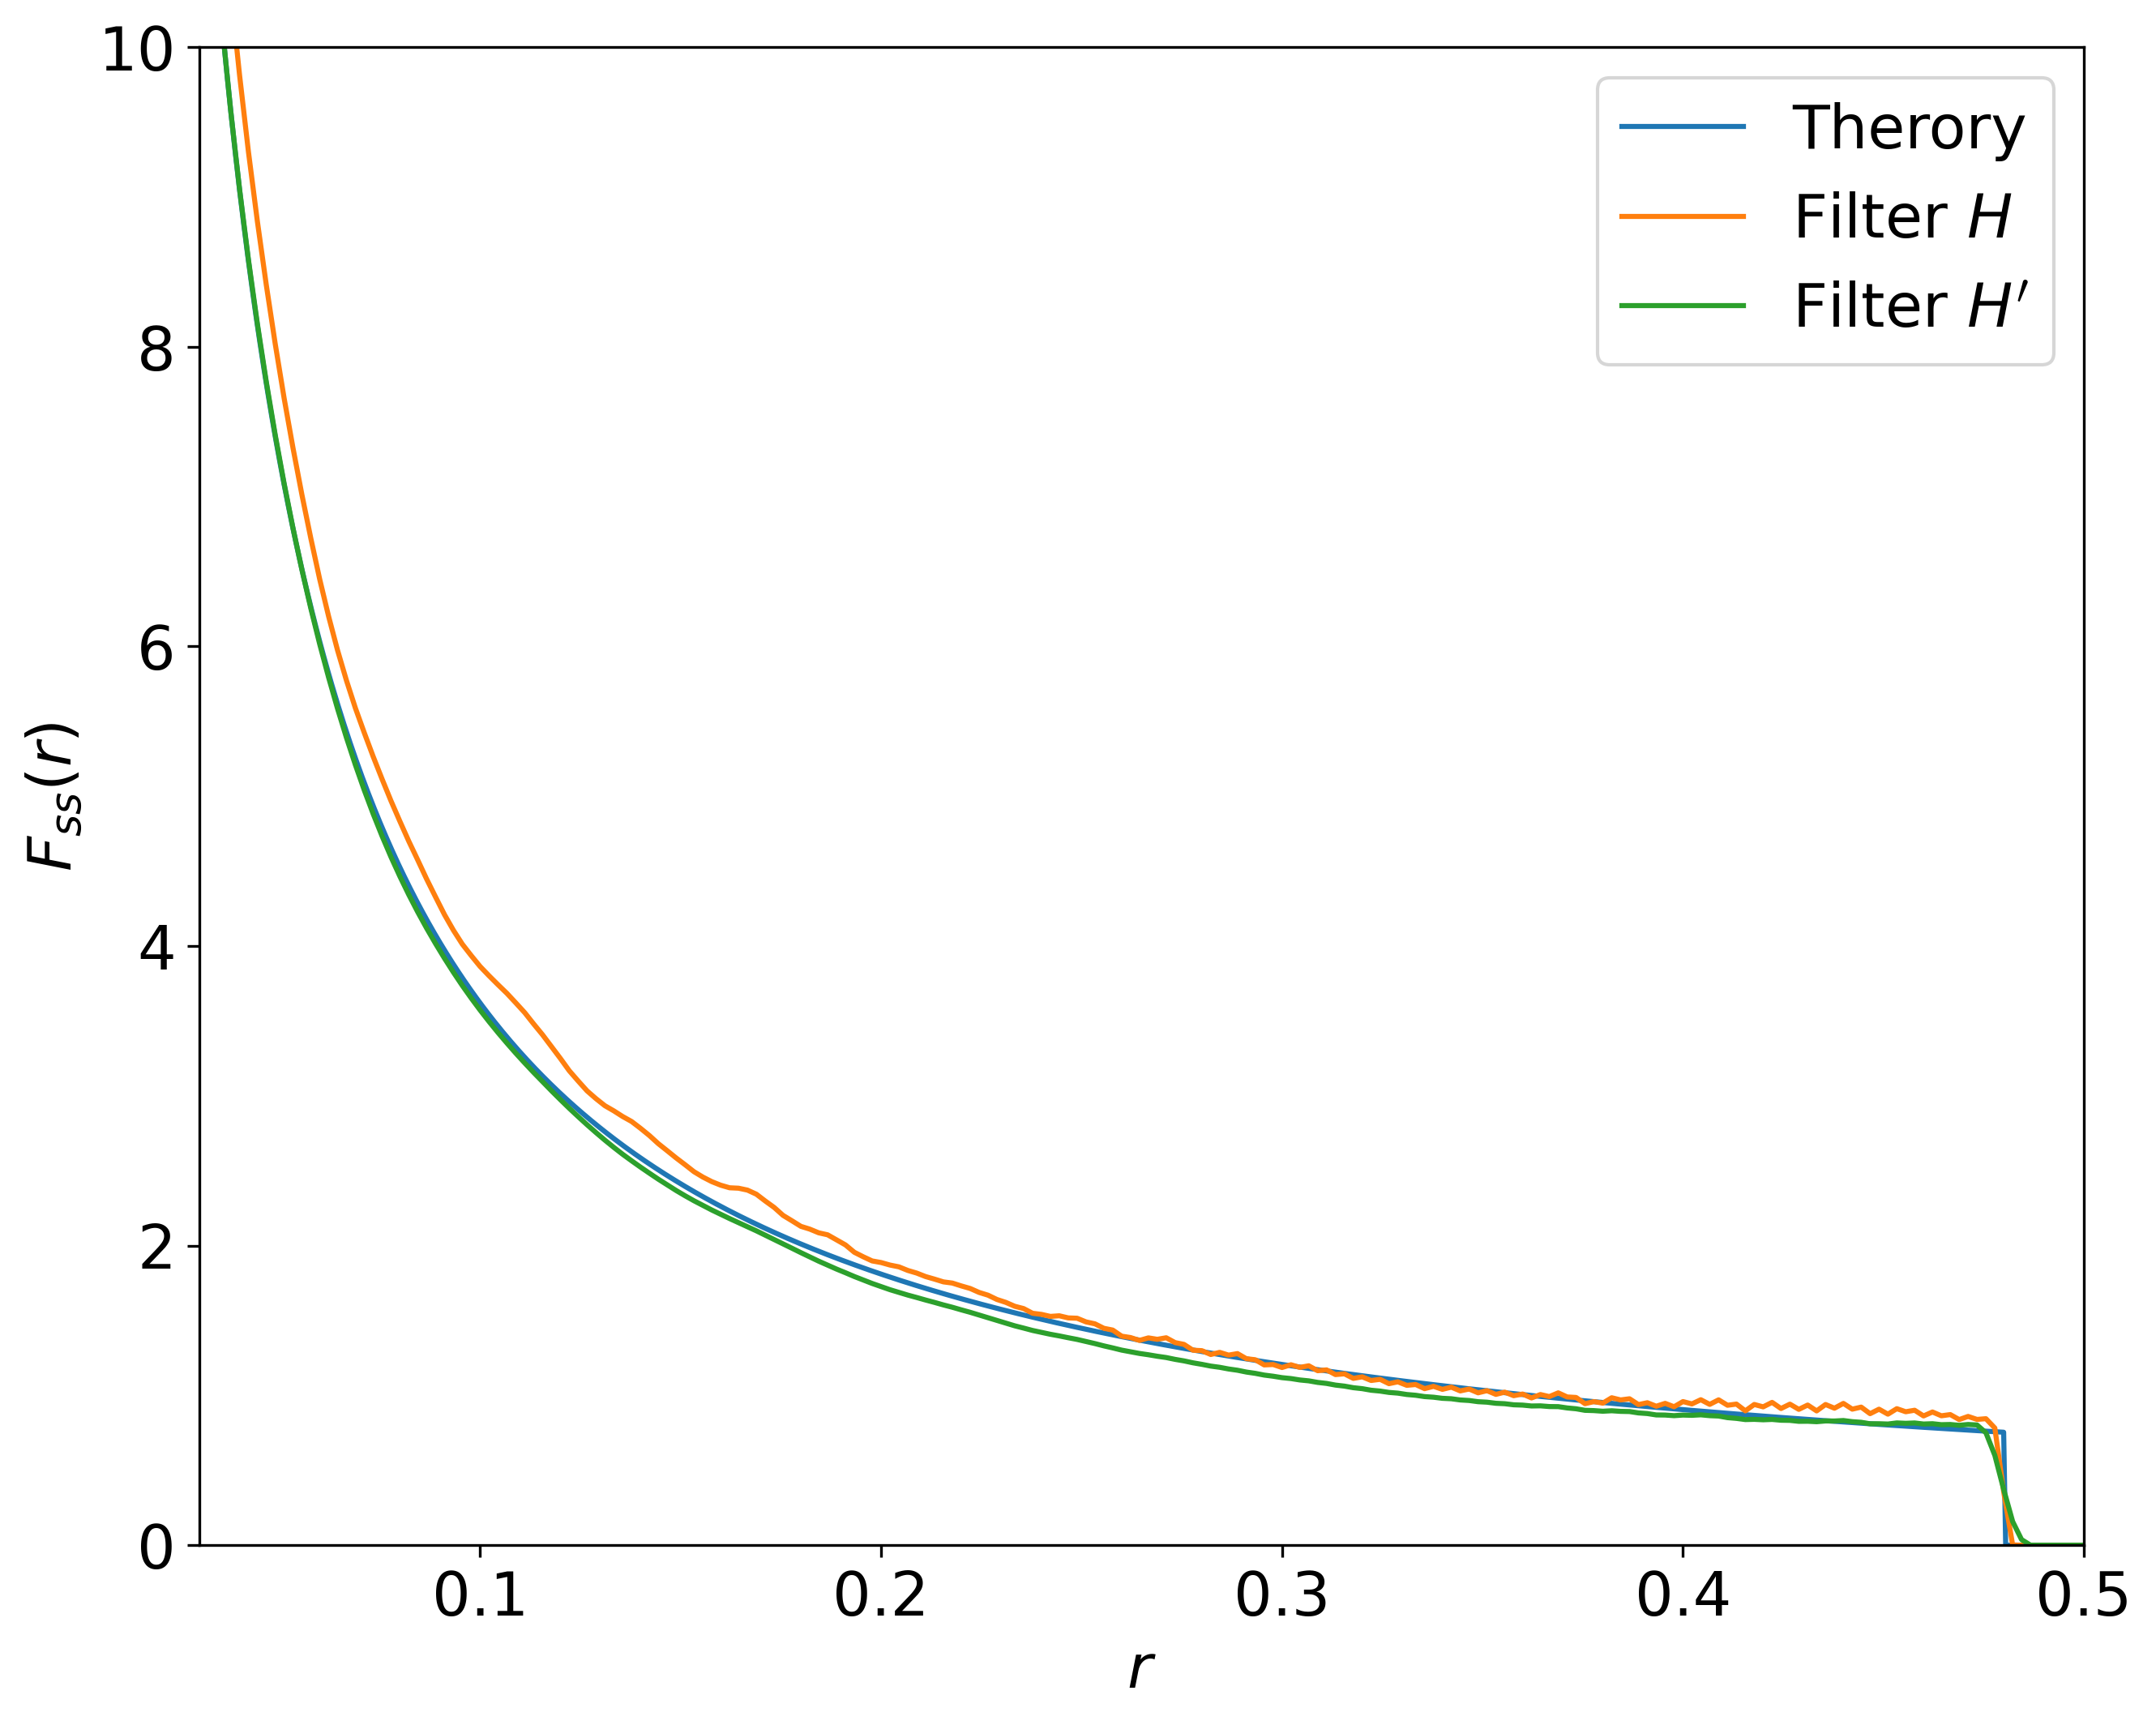
\includegraphics[width=0.45\linewidth]{images/ball-3d-ss.png}
    \label{fig:fss-ball}}
  \hfill
  \subfigure[Surface-void function calculated for a disk with radius
    $R = 0.2$. Image dimensions are $2000 \times 2000$.]{
    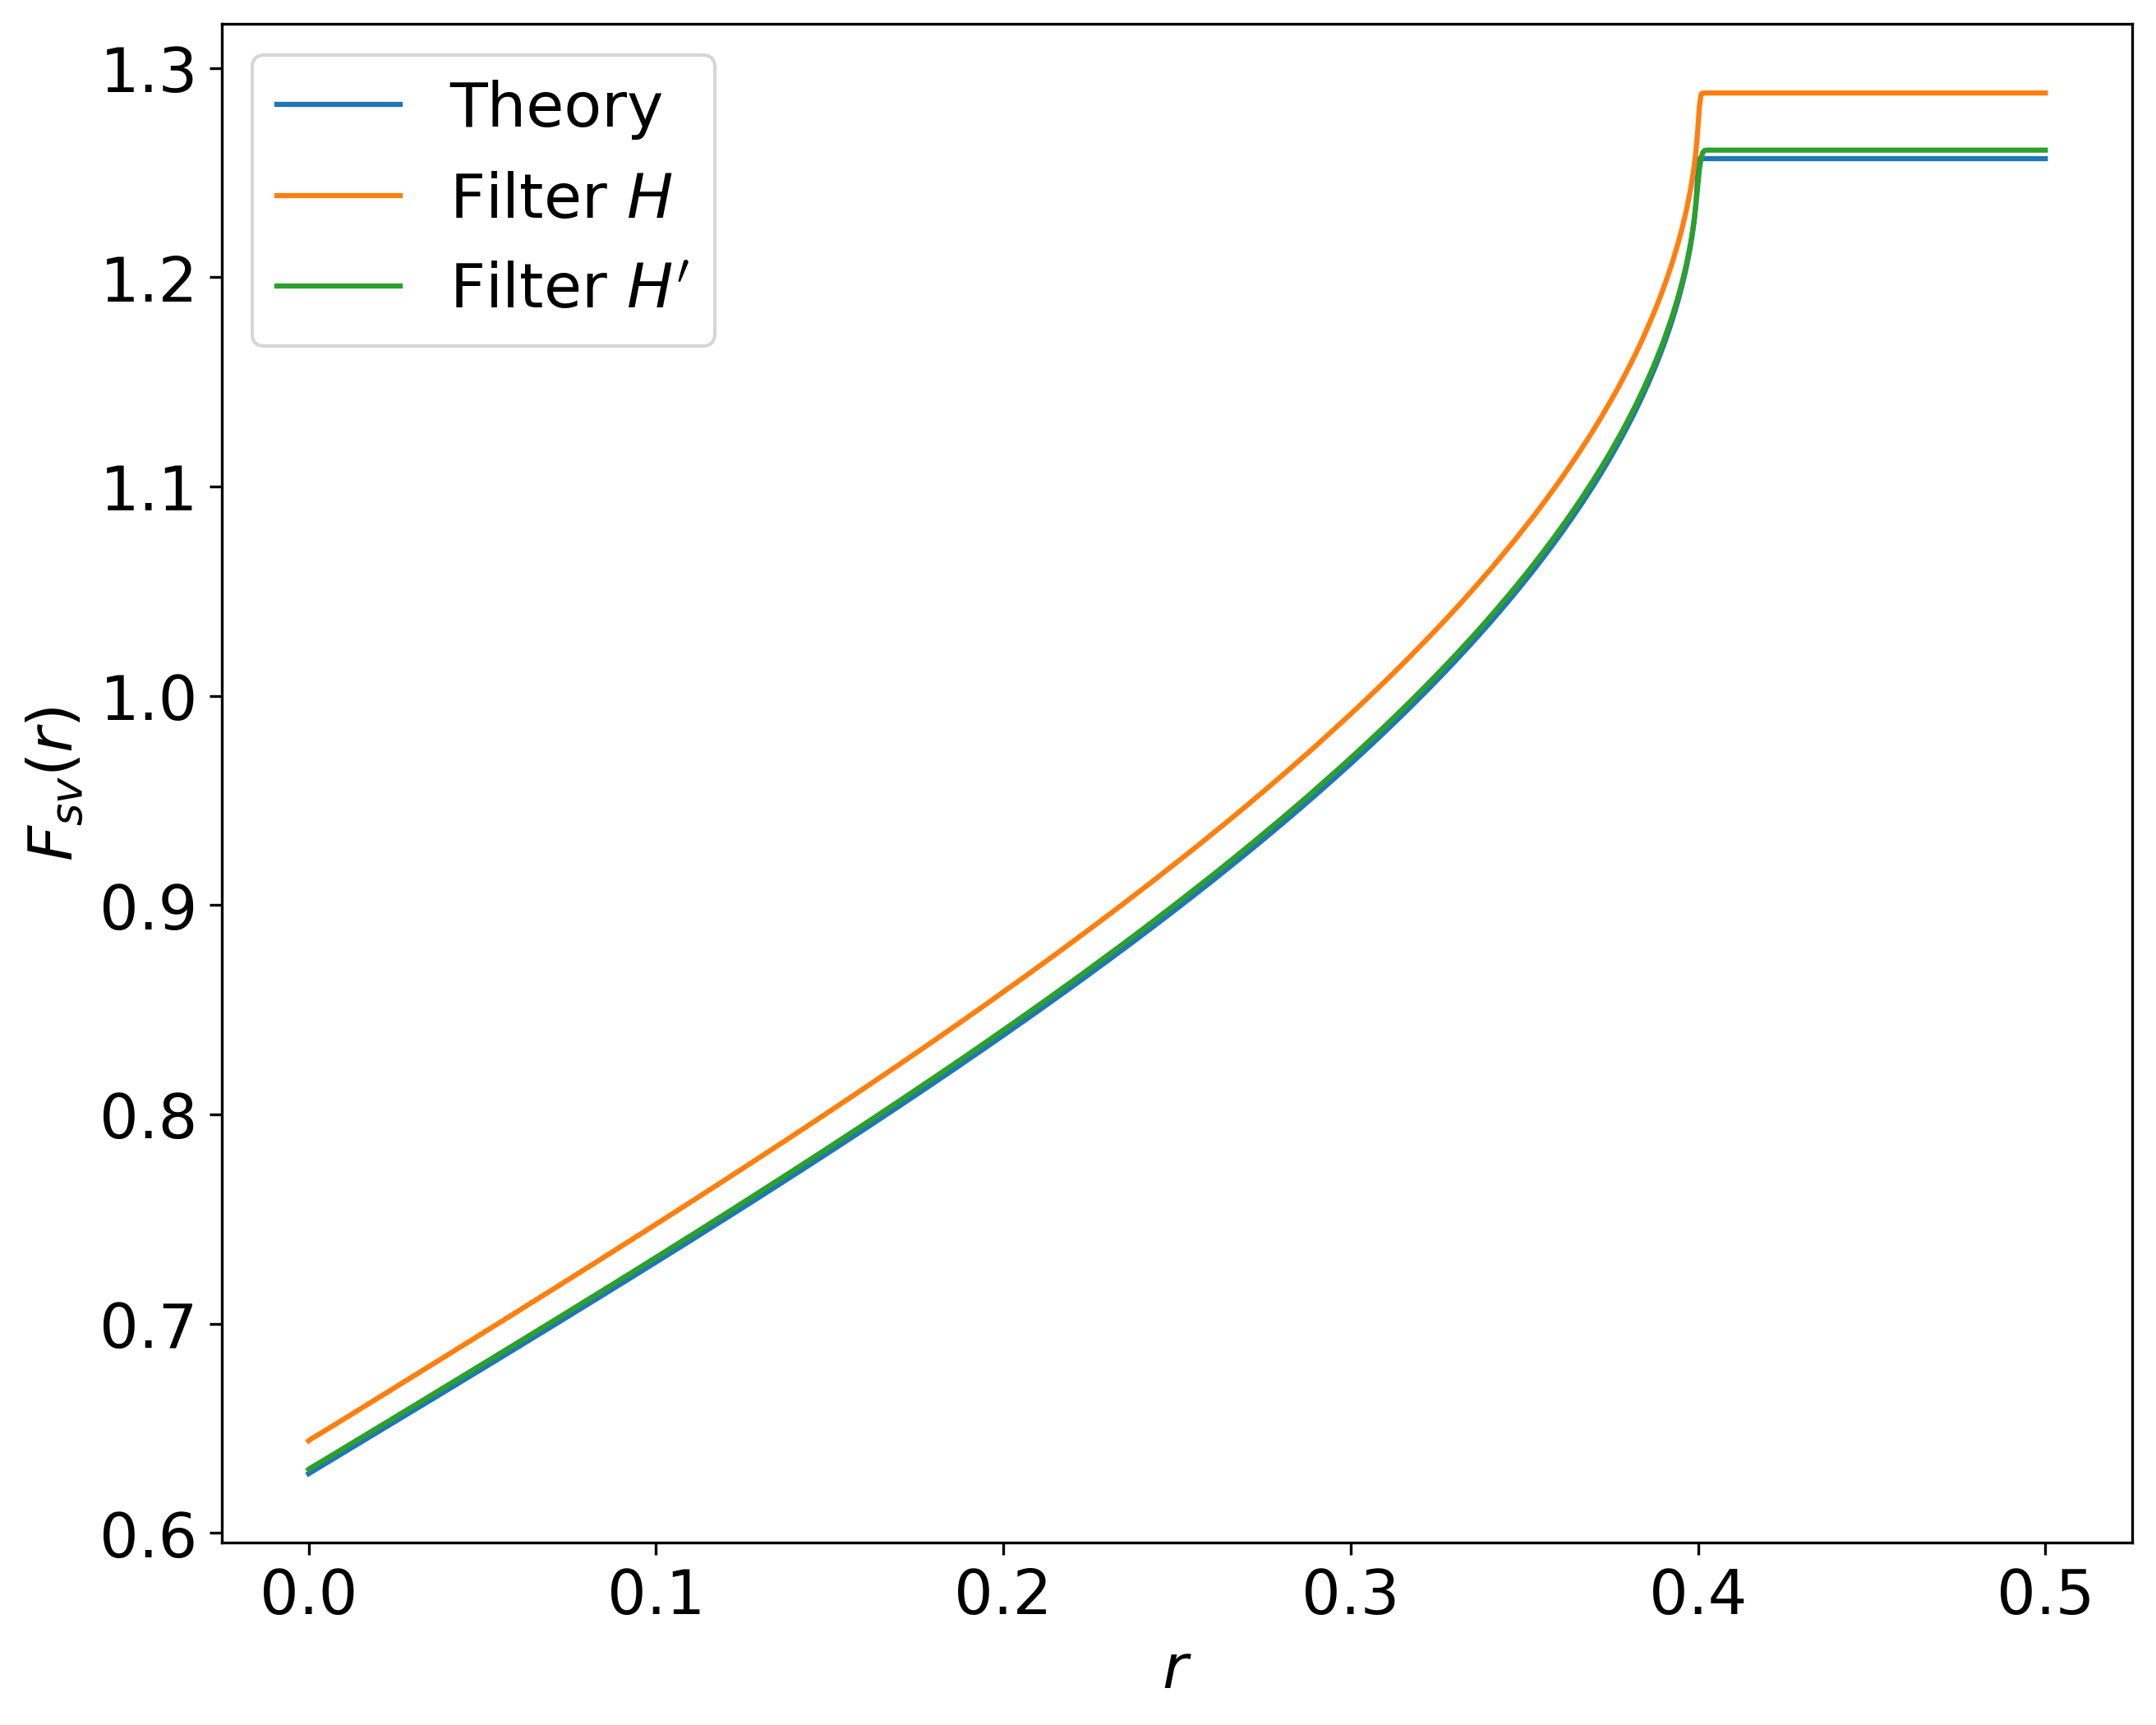
\includegraphics[width=0.45\linewidth]{images/fsv-disk.png}
    \label{fig:fsv-disk}}
  \vskip\baselineskip
  \subfigure[Surface-void function calculated for a ball with radius
    $R = 0.2$. Image dimensions are $300 \times 300 \times 300$.]{
    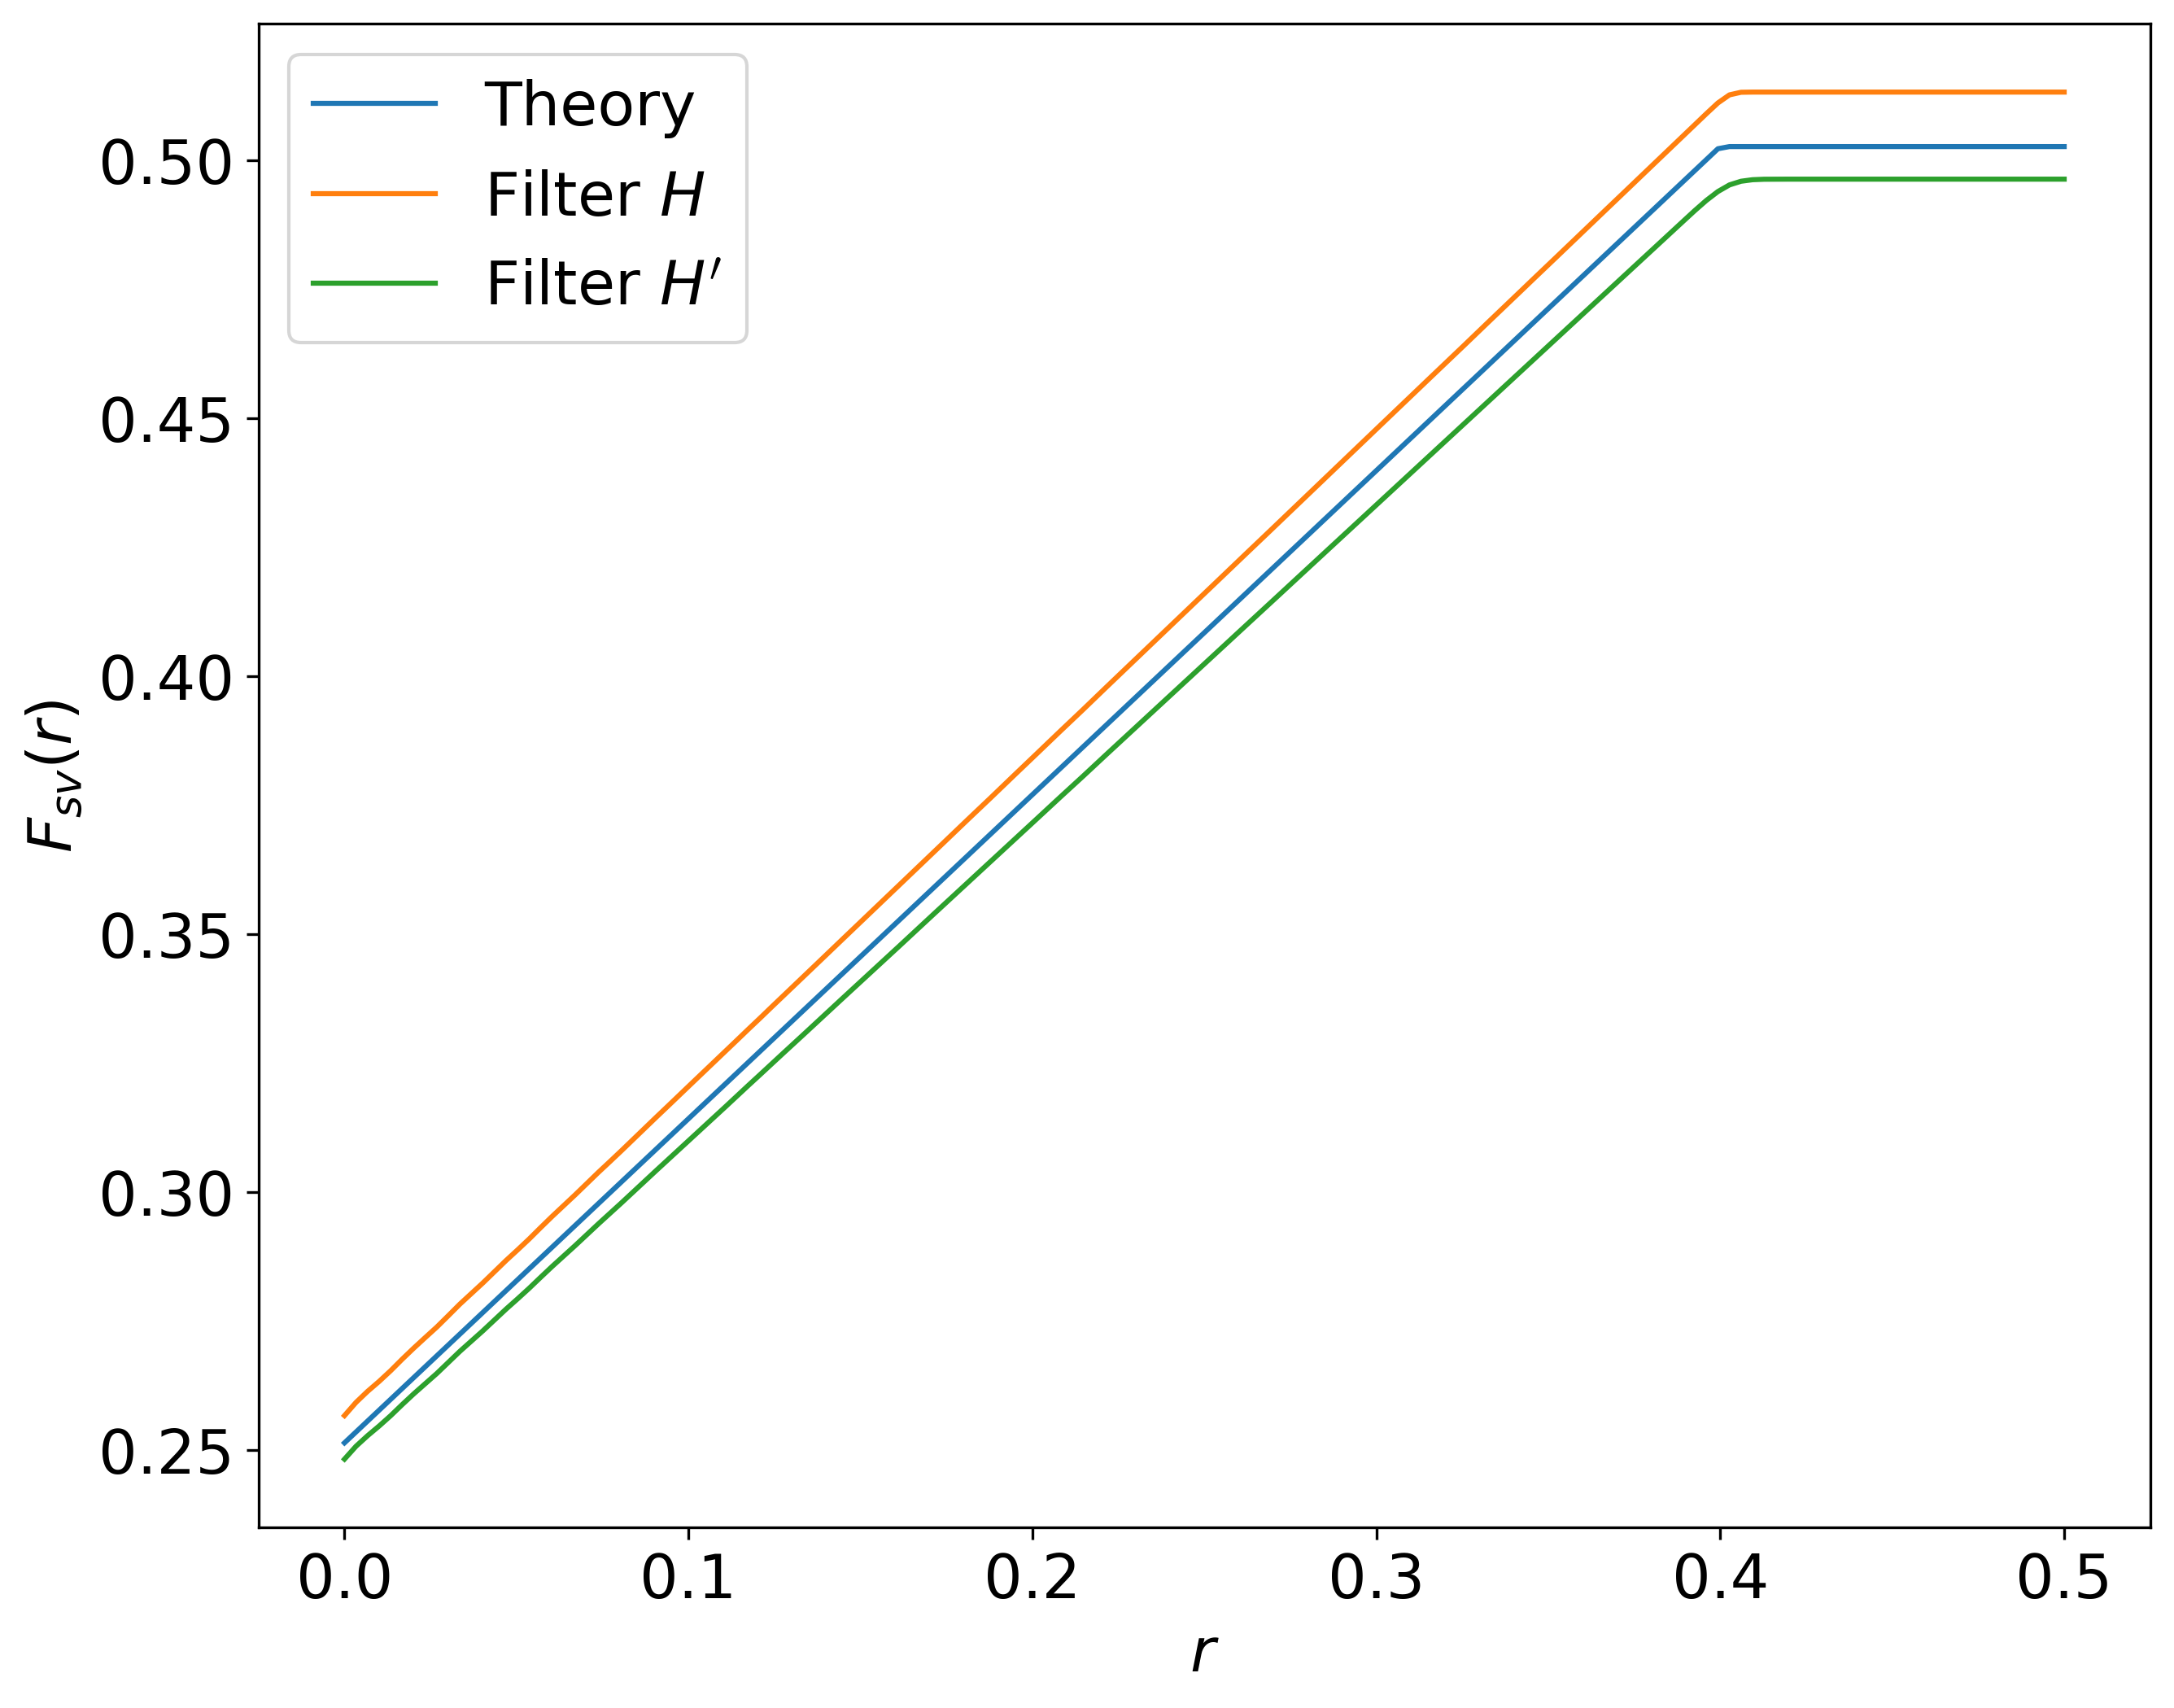
\includegraphics[width=0.45\linewidth]{images/fsv-ball.png}
    \label{fig:fsv-ball}}
  \caption[]{Comparison of filters $H$ and $H'$ for cases in which newly
    developed algorithms \cref{sec:fss-2d}, \cref{sec:fsss-3d} are not
    applicable. Theoretical curves are provided for each case.}
  \label{fig:not-covered}
\end{figure*}
With the new filter the calculation of $F_{ss}$ becomes more precise also for
three-dimensional images. This can be seen in comparison with theoretical values
for known cases, e.g., a ball. On \cref{fig:fss-ball} plots
of $F_{ss}$ function calculated with filters $H$ and $H'$ along with a
theoretical curve are presented. It can be verified that filter $H'$ is indeed results 
in higher accuracies with the help of error metric:
\begin{equation}
  error = \sqrt{\frac{\sum_i (F_{ss}^{calc}(x_i) -
      F_{ss}^{theory}(x_i))^2}{\sum_i F_{ss}^{theory}(x_i)^2}}
  \label{eq:error}
\end{equation}
where $x_i$ belong to a set $(\epsilon, 2R - \epsilon)$. Taking
$\epsilon = 0.01$ we obtain the error equal to 0.05 for filter $H$ and 0.03 for
filter $H'$, respectively. Calculation of surface-void function also benefits
from the new filter (\cref{fig:fsv-disk}, \cref{fig:fsv-ball}).

However, the $H'$ filter has some drawbacks as compared to $H$. Firstly, $H$ has
faster convergence with increase of image resolution. Secondly, $H'$ behaves
worse than $H$ in points of discontinuity of $F_{ss}$ as can be seen on
\cref{fig:fss-disk}. To explore such effects we appeal to the parameter
$C_\alpha$ \cite{Samarin} developed to determine if an image is suitable for
robust assessment of surface correlation functions. To introduce this parameter,
consider a continuos band-limited signal $f(t)$ with support in frequency domian
$[-\omega_0, \omega_0]$. The $L^2$ norm of this signal is:
\begin{equation}
  \|f\| = \sqrt{\int_{-\omega_0}^{\omega_0} |\hat{f}(\omega)|^2 d\omega}
\end{equation}
where $\hat{f}(\omega)$ is a Fourier transform of $f(t)$. The idea behind the
parameter is to determine how much low-frequency domain contributes to the total
power of a signal. $C_\alpha$ parameter is defined as:
\begin{equation}
  \begin{aligned}
    C_\alpha &= \sqrt{\frac{\int_{-\alpha\omega_0}^{\alpha\omega_0}
        |\hat{f}(\omega)|^2 d\omega}{\int_{-\omega_0}^{\omega_0}
        |\hat{f}(\omega)|^2 d\omega}} \\
    \alpha &\in [0, 1]
  \end{aligned}
  \label{eq:parameter}
\end{equation}
For two- and three-dimensional discrete images $f(t)$ is replaced with the input
array $A$ minus its mean, integrals in \cref{eq:parameter} are replaced with
double and triple sums respectively and $\omega_0$ is equal to the Nyquist
frequency for the image. Our empirical criterion says that the image is suitable
for evaluation of surface correlation functions if:
\begin{equation}
  C_{0.5} > 0.97
\end{equation}
This criterion works for both filters $H$ and $H'$, but $H$ results in smaller
error when $C_{0.5}$ is slightly less than 0.97. For example, consider images of
a disk used for calculation of $F_{ss}$ on \cref{fig:fss-disk}. On
\cref{fig:error} we provide values of $C_{0.5}$ for this image (for variety of
resolutions) and relative errors in $F_{ss}$ (\cref{eq:error}) for both
filters. It can be seen that $H$ gives twice the lower error than $H'$ when used
for an image with $C_{0.5} \approx 0.82$. In short, for images of acceptable
quality the $H'$ filter is superior.

\begin{figure*}[!hpt]
  \centering
  \subfigure[$C_{0.5}$ criterion]{
    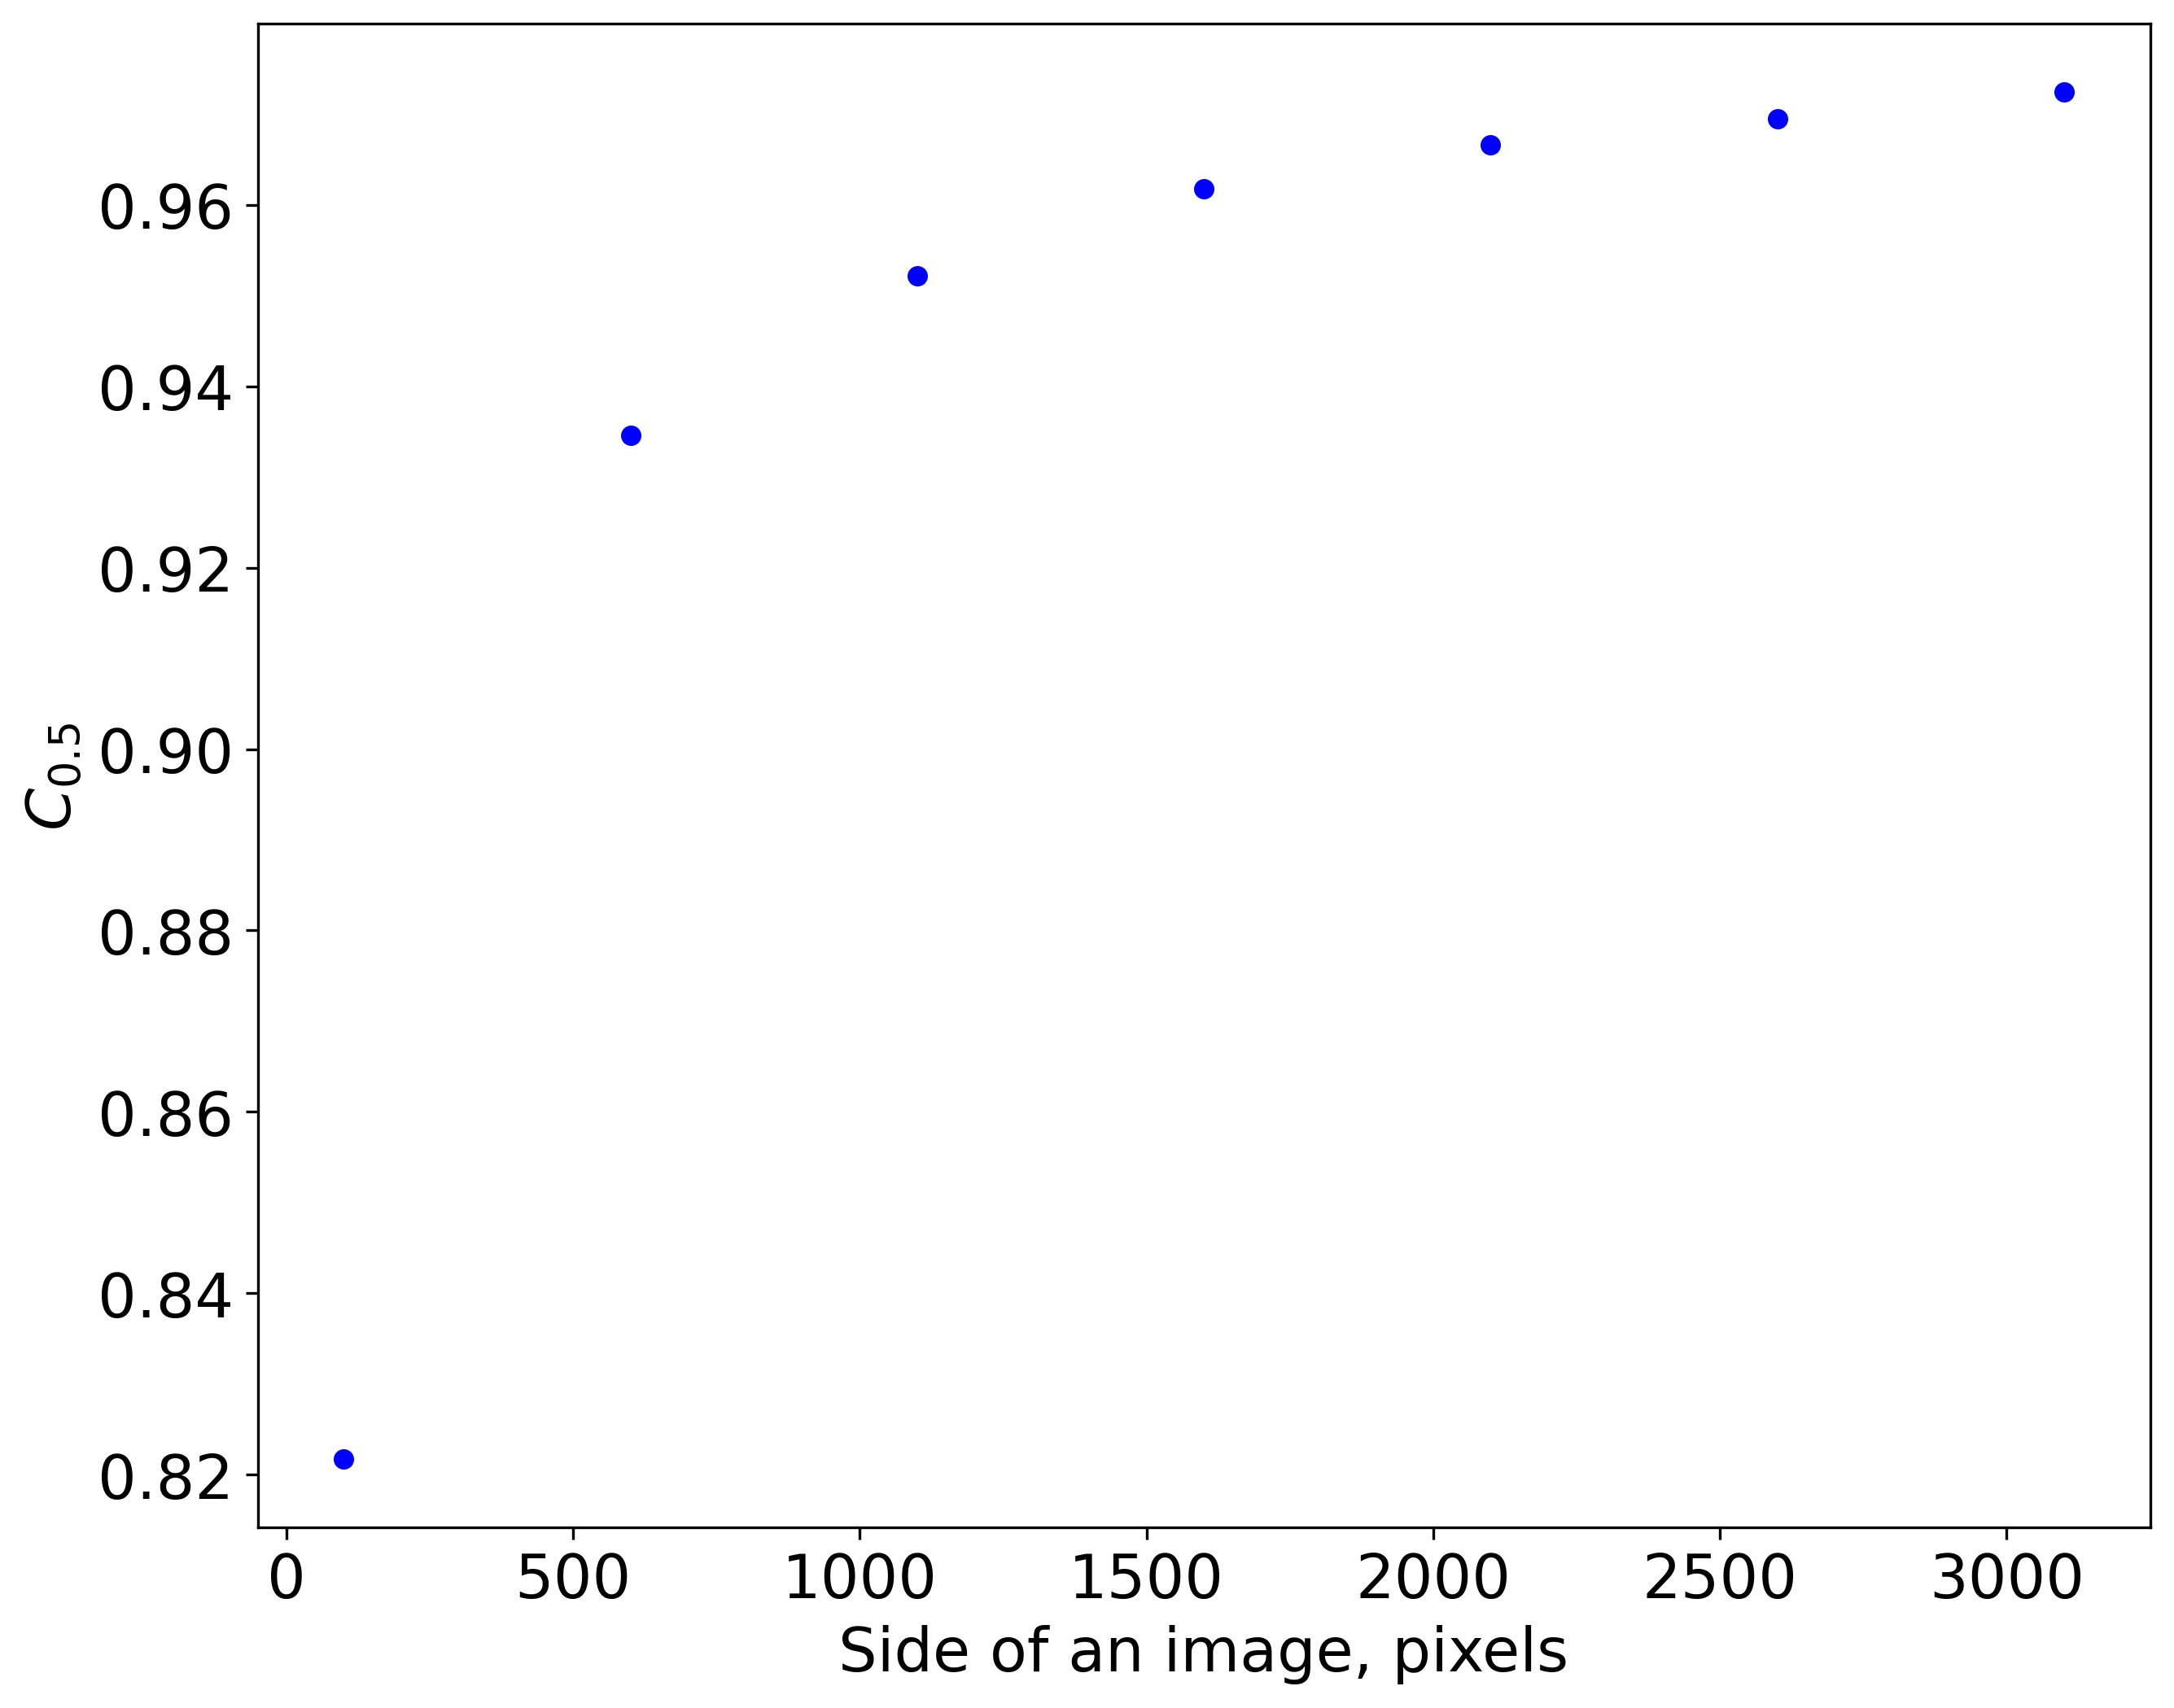
\includegraphics[width=0.45\linewidth]{images/c05.png}
    \label{fig:c05}}
  \hfill
  \subfigure[Relative errors in computation of $F_{ss}$]{
    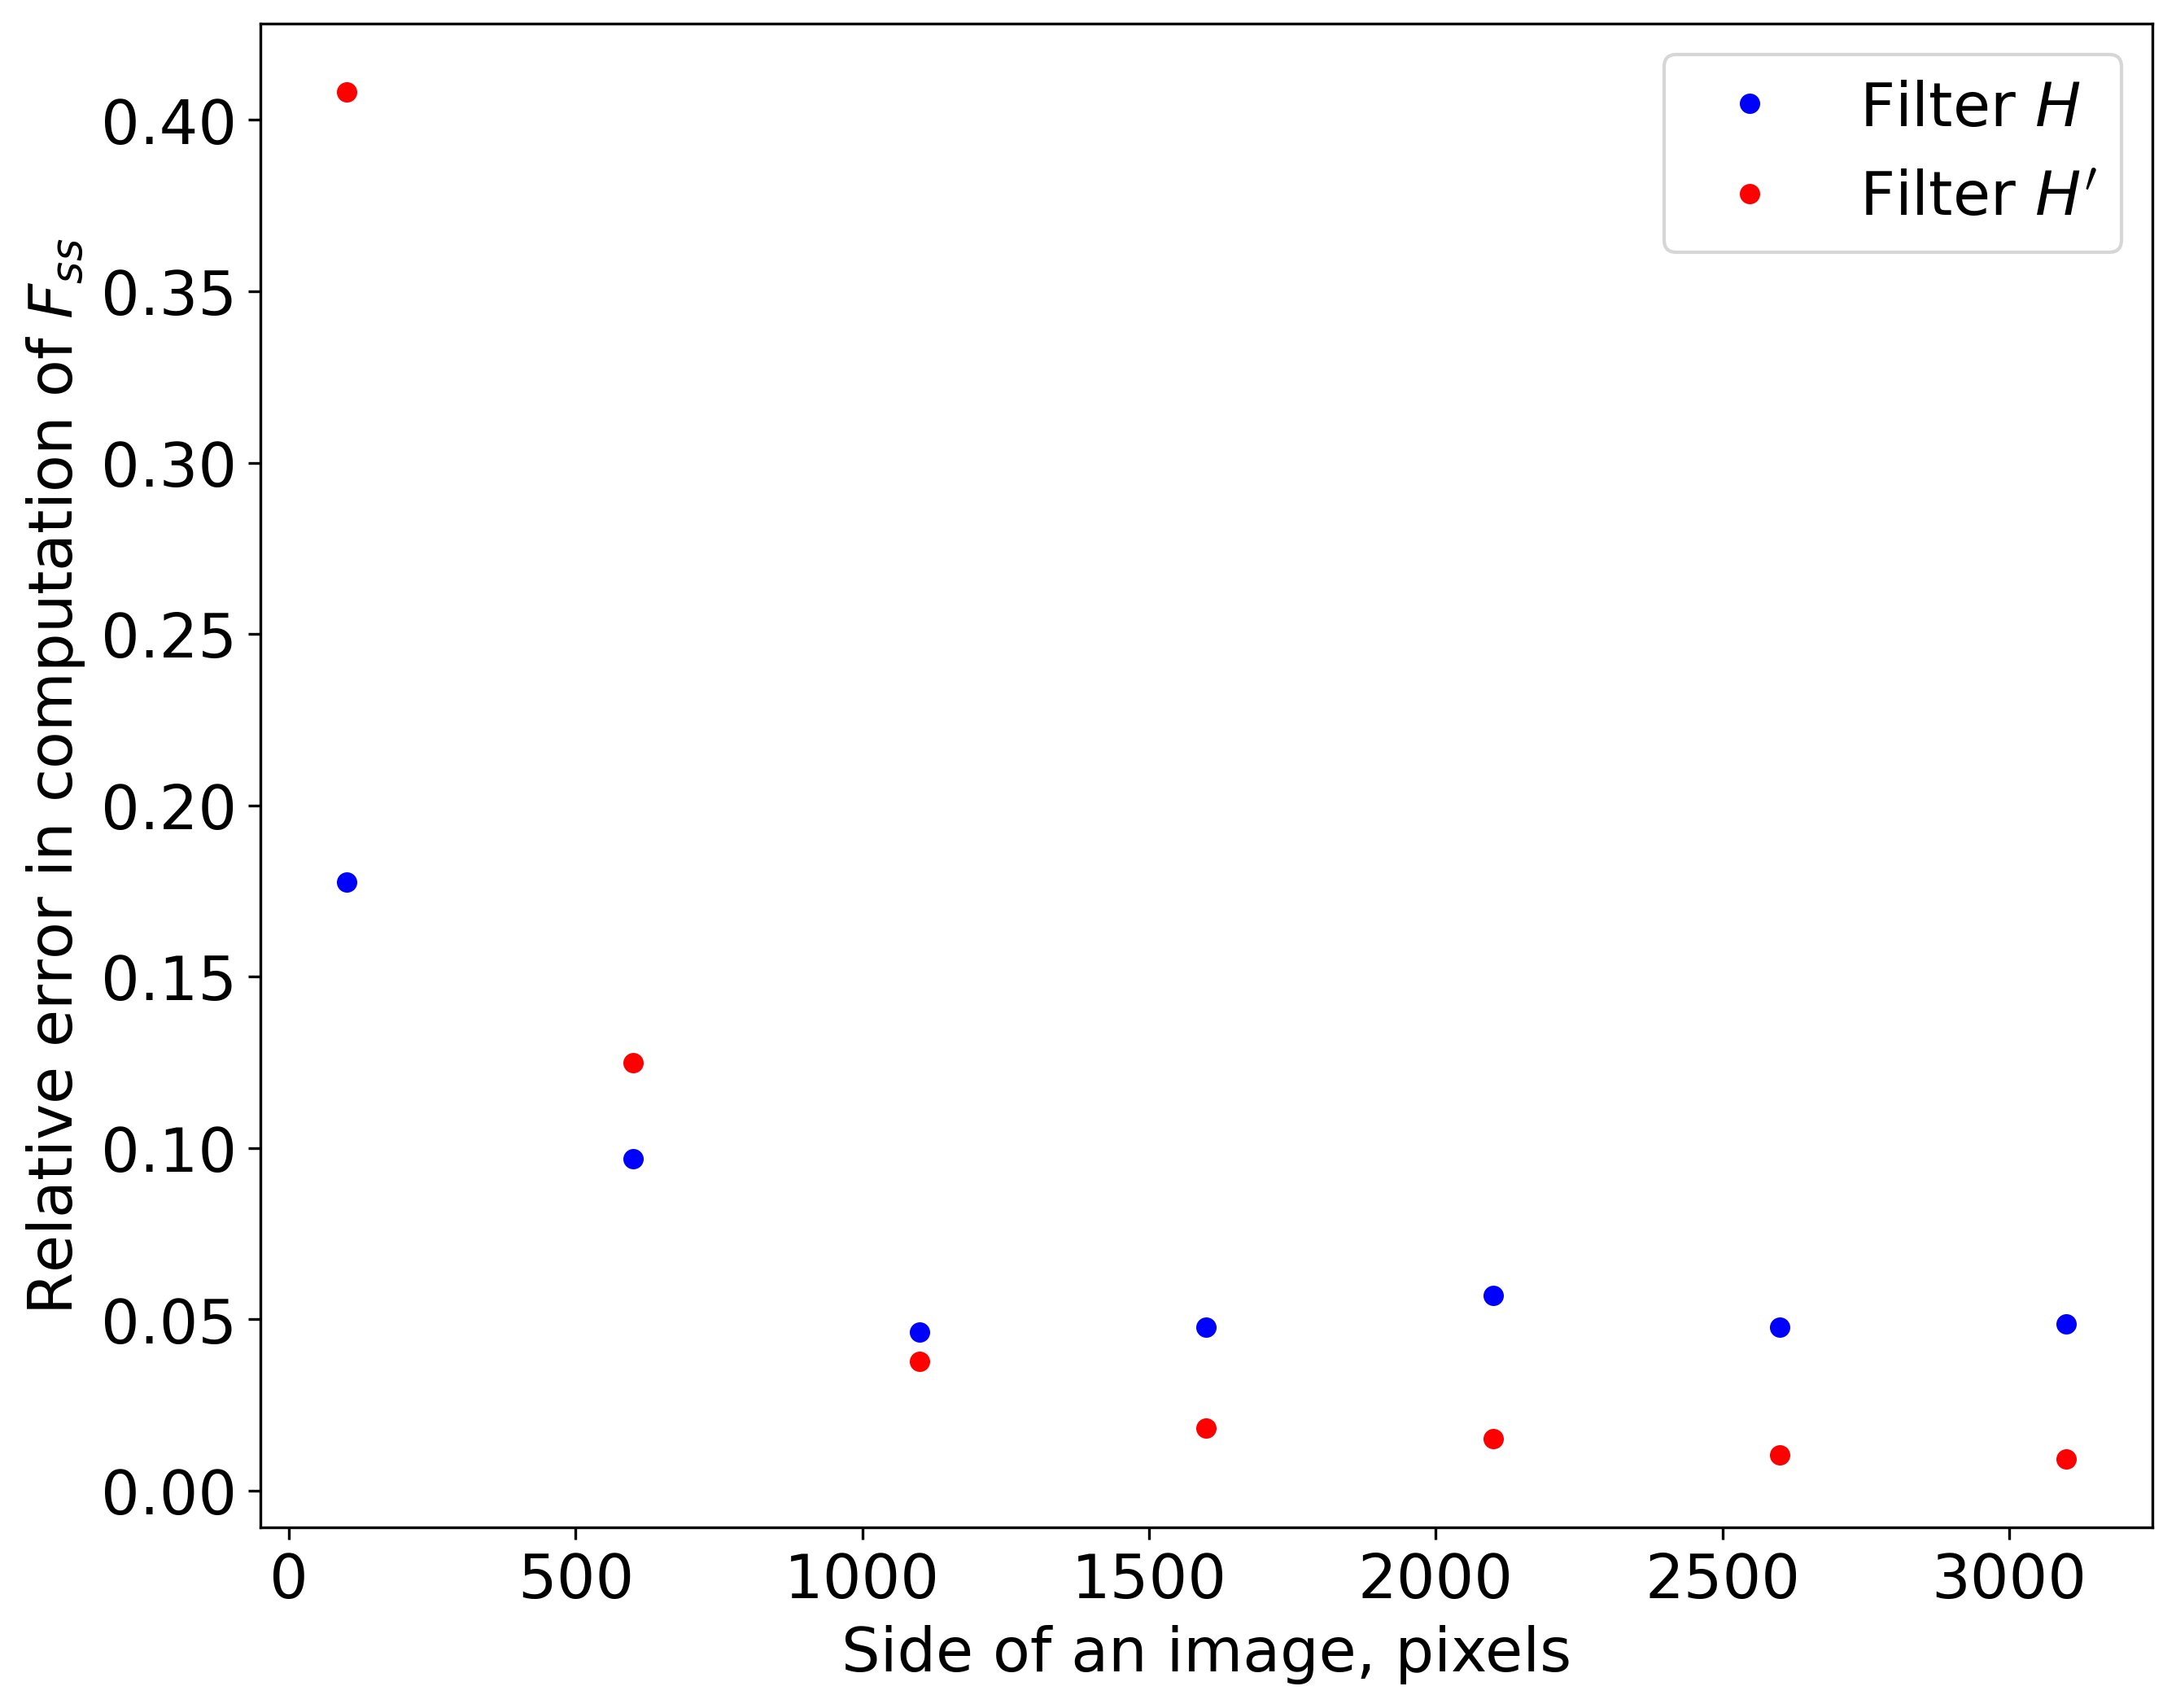
\includegraphics[width=0.45\linewidth]{images/fss-disk-errors.png}
    \label{fig:relerr}}
  \caption[]{Relative errors in function $F_{ss}$ for the case of a disk
    (\cref{fig:fss-disk}) for filters $H$ and $H'$ and the acceptance parameter
    $C_{0.5}$.}
  \label{fig:error}
\end{figure*}

\section{Discussion, outlook and summary}
\label{sec:summary}
The exact continuous method presented in this paper is developed only for
surface-surface function (and its 3-point counterpart). The surface-void
function computations in digital manner are much more robust and exhibit less
perturbation \cite{ma2018SS,Samarin}. The filter $H'$ verified for $F_{ss}$ also
improves calculations for $F_{sv}$ (as evident from \cref{fig:not-covered}).

In addition to obvious applications of surface correlations, as described in
\cref{sec:intro}, the development of robust computation techniques opens
interesting research directions:
\begin{enumerate}
    \item Possibility to evaluate surface functions from small-angle scattering
      experiments \cite{dietrich1995scattering};
    \item Finding overall trends in porous media structural evolution, e.g.,
      based on experimental datasets \cite{noiriel2021pore,fomin2023};
    \item Qualitative exploration of molecular scale roughness effects on electric 
      double layer structure in asymmetric ionic liquids \cite{aslyamov2021,khlyupin2023}.
\end{enumerate}
This list immediately pops up from the authors' research activities and is,
potentially, much wider.

In summary, here we developed novel algorithm for precise calculation of
$F_{ss}$ function for two-dimensional sets and $F_{sss}$ function for
three-dimensional sets. These sets must have smooth boundary for the algorithm
to be applicable. With help of this new algorithm we introduced some additional
testing techniques for digital computational methodology, including concave
surface shapes.  In particular, we were able to demonstrate the improvement in
calculations of surface-surface and surface-void correlation functions for
digital binary images with the help of proposed $H'$ filter.

An implementation of the precise continuous algorithm in Common Lisp for sets
with smooth boundary is available on GitHub
\cite{diff-boundary-corrfn}. Improved digital approach for both $F_{ss}$ and
$F_{sss}$ is now part of open source package CorrelationFunctions.jl written in
Julia \cite{CFs.jl}.

\section{Acknowledgements}
This research was supported by the Russian Science Foundation grant 23-74-00061. Collaborative effort of the authors is within the FaT iMP 
(Flow and Transport in Media with Pores) research group (www.porenetwork.com). We thank our colleague Konstantin Romanenko for suggestions 
and administrative work.

\bibliography{paper}

\appendix
\section{Dual numbers and automatic differentiation}
\label{sec:dual}
A ring of dual numbers $D$ is a set of pairs of real numbers $(a, b)$ with two
binary operations: $+$ (addition) and $\cdot$ (multiplication) where
multiplication works according to the following law:
\begin{equation}
  (a, b)\cdot(c, d) = (ac, ad + bc)
\end{equation}
It's easy to see that $D$ is commutative.

It is also useful to introduce an imaginary unit $\varepsilon$ and write a dual
number $(a, b)$ as $a + b\varepsilon$. As follows from the multiplication law,
$1\cdot \varepsilon = \varepsilon$ and $\varepsilon^2 = 0$, hence $D$ is not an
integral domain and division is defined only if divisor has non-zero real part:
\begin{equation}
  \begin{aligned}
    \frac{a+b\varepsilon}{c+d\varepsilon} &=
    \frac{(a+b\varepsilon)(c-d\varepsilon)}{(c+d\varepsilon)(c-d\varepsilon)} \\
    &= \frac{ac-ad\varepsilon+bc\varepsilon}{c^2} \\
    &= \frac{a}{c} + \frac{bc-ad}{c^2}\varepsilon
  \end{aligned}
\end{equation}

Now we consider functions of dual variable $x + y\varepsilon$. Power function
$(x + y\varepsilon)^n$ where $n \in \mathbb{N}$ can be defined using binomial
formula and keeping in mind that $\varepsilon^n = 0$ if $n>1$:
\begin{equation}
  (x + y\varepsilon)^n = \sum_{k=0}^n \binom{n}{k} x^k (y\varepsilon)^{n-k} =
  x^n + n x^{n-1} y \varepsilon
\end{equation}
This formula can be extended to $n \in \mathbb{Q}$ as well.

Elementary functions can be extended to dual numbers using Taylor series (here
$a$ is some point at which $f$ is differentiable):
\begin{equation}
  \begin{aligned}
    f(x + y\varepsilon) &= f(a) + f'(a)(x + y\varepsilon) + \frac{f''(a)}{2!}(x + y\varepsilon)^2 \\
    & \qquad + \frac{f'''(a)}{3!}(x + y\varepsilon)^3 + \dots \\
    &= f(a) + f'(a)(x + y\varepsilon) + \frac{f''(a)}{2!}(x^2 + 2xy\varepsilon) \\
    & \qquad + \frac{f'''(a)}{3!}(x^3 + 3x^2y\varepsilon) + \dots \\
    &= f(a) + f'(a)x + \frac{f''(a)}{2!}x^2 + \frac{f'''(a)}{3!}x^3 + \dots \\
    & \quad y\varepsilon(f'(a) + f''(a)x + \frac{f'''(a)}{2!}x^2 + \dots) \\
    &= f(x) + yf'(x)\varepsilon
  \end{aligned}
\end{equation}

Most useful basic rules for working with dual numbers can be summarized as follows:
\begin{itemize}
\item $(a + b\varepsilon) + (c + d\varepsilon) = (a + c) + (b + d)\varepsilon$
\item $(a + b\varepsilon) (c + d\varepsilon) = ac + (ad + bc)\varepsilon$
\item $\frac{a + b\varepsilon}{c + d\varepsilon} = \frac{a}{c} + \frac{bc - ad}{c^2}$
\item $\exp(a + b\varepsilon) = \exp(a) + b\varepsilon\exp(a)$
\item $\sin(a + b\varepsilon) = \sin(a) + b\varepsilon\cos(a)$
\item $\cos(a + b\varepsilon) = \cos(a) - b\varepsilon\sin(a)$
\item $\tan(a + b\varepsilon) = \tan(a) - \frac{b}{cos^2(a)}\varepsilon$
\end{itemize}

As is evident from these rules, dual numbers are connected with
differentiation. Using a dual argument $a + \varepsilon$ we can compute a value
of a function at point $x = a$ and its derivative at that point:
$f(a + \varepsilon) = f(a) + f'(a)\varepsilon$. Also, we can compute a partial
derivative of a multivariate function. For example:
\begin{equation}
  \begin{aligned}
    \frac{\partial}{\partial x} f(x, y) \vert_{x = a, y = b} &= f(a + \varepsilon,
    b) \\
    \frac{\partial}{\partial y} f(x, y) \vert_{x = a, y = b} &= f(a, b +
    \varepsilon)
  \end{aligned}
  \label{eq:autonormals}
\end{equation}
This last equation is the main result of this appendix and can be used for
computation of normals to the interface.

\end{document}
